\documentclass{kththesis}

\justifying
\usepackage{graphicx}
\usepackage{epigraph}
\usepackage{bm}
\usepackage{hyperref}
\usepackage{todo}
\usepackage{subcaption}
\usepackage{float}
\usepackage[chapter]{algorithm}
\usepackage{algorithmic}
\usepackage{amsmath}
\usepackage{multirow}
\usepackage{booktabs}
\usepackage{adjustbox}

% remove this if you are using XeLaTeX or LuaLaTeX
\usepackage[utf8]{inputenc}

% Use natbib abbreviated bibliography style
\usepackage[square,numbers]{natbib}
\bibliographystyle{unsrtnat}

\usepackage{lipsum} % This is just to get some nonsense text in this template, can be safely removed

\title{Sequential User Retention Modelling}
\alttitle{Detta är den svenska översättningen av titeln}
\author{Helder Martins}
\email{helder@kth.se}
\supervisor{Hedvig Kjellström (KTH) and Sahar Asadi (Spotify)}
\examiner{Patric Jensfelt}
\programme{Master in Machine Learning}
\school{School of Computer Science and Communication}
\date{\today}


\begin{document}

% Title page
\flyleaf

\begin{abstract}
  English abstract goes here.
\end{abstract}

\clearpage

\begin{otherlanguage}{swedish}
  \begin{abstract}
    Träutensilierna i ett tryckeri äro ingalunda en faktor där
    trevnadens ordningens och ekonomiens upprätthållande, och dock är
    det icke sällan som sorgliga erfarenheter göras ordningens och
    ekon och miens därmed upprätthållande. Träutensilierna i ett
    tryckeri äro ingalunda en oviktig faktor, för trevnadens
    ordningens och och dock är det icke sällan.
  \end{abstract}
\end{otherlanguage}

\cleardoublepage

\tableofcontents


% This is where the actual contents of the thesis starts
\mainmatter


\chapter{Introduction}

	This chapter will be dedicated to introduce the topic of this thesis project, the motivations on why it is relevant to both academia and to the industry, the current context where this project is being developed on, the hypothesis that shall be explored, the methodology used to verify it, and the contributions of this work.
	
	The rise of streaming services has in recent years revolutionized the way customers get access to digital content. The traditional model of media ownership, even though it still represents a significant share of revenue, is continuously losing ground to a new right-of-access model where users get access to content ether by paying a monthly subscription or by being exposed to advertisement. The customer base of said services is steadily growing, and with it the amount data collected tracking how they interact with the provided digital media. This information is of high-value to any provider who expects improve the user experience, increase its total number of clients and also avoid losing the current ones to the competition.
	
	One application of a data set based on historical user behaviour that has received attention from the industry is to predict the clients that are more likely to leave the service in the near future and anticipate it by performing a set of actions with the goal of avoiding it from happening. It is predicted that there is a set of features which are highly correlated with their desire of abandoning the application, and thus a model could be trained to leverage this information and classify users based on the probability of that event occurring. Such models are called \emph{churn predictors}, and will be a central subject on this thesis project. Another interest will be to evaluate which set of features among the available ones actually correlates with churn and extract from it actionable insights that can be suggested to the provider as a form of improvement to their application, a task made harder by the extremely large number of attributes that is commonly captured.
	 
	Predicting whether a user is going to leave the service provider in the near future is a subject that has received some attention in the academia in the past few years \Todo{add ref}. Most of them share however a common trait regarding the way the data is represented before being used for model training: the data is split into \emph{time windows} spanning different time ranges (usually one after the other), where an older time window used for model training and a time window closer to the present date to verify whether the observed user is going to churn or not. The common approach for dealing with the user data that is by nature sequential is by aggregating the feature values into a single representation for each user, normally through a mean function. Even though this approach simplifies the task of training the predictor models, latent temporal factors hidden in the sequence that could prove useful for increasing the performance of models are inherently lost in this process. One of the hypothesis that is going to be explored in this project is if using the raw sequential data and also a predictor model that knows how to leverage this property, a significant performance gain can be achieved when comparing to a state-of-the-art baseline model.
	 
	The user behaviour data and the required computational resources were provided by \emph{Spotify}, a well known music streaming service that joined this project in a tutoring partnership with the student and the university. Creating a suitable data set for training our proposed models is also part of the project, and it was performed by first exploring the data at our disposal and identifying the features that highly correlates with churn. While the available data is mostly related to the music domain, the methodology of this project and the conclusions reached can also be extended to other domains like video streaming with minor modifications.
	
	
	\section{Streaming services}

	The last decade has witnessed an overwhelming increase in popularity in all kinds of streaming services around the globe. Applications like Netflix and Spotify have changed the industry by offering a legal and affordable way of accessing content through a subscription-like contract instead of the classical pay-by-content commonly used by traditional media providers. This change in business model has proven to be successful by the sheer amount of customers that the most popular service providers have nowadays. Netflix for instance has reported to its shareholders a user base of 93 million worldwide at the end of 2016 \citep{netflixsh}, while Spotify recently reached the amazing feat of 50 millions paying subscribers, 20 millions of that only in one year \citep{spotifypress}. Even though bureaucratic challenges like the dispute between the service providers and the labels regarding the value of licenses are still on debate, the adoption of this new model by consumers indicates no interest of going back to the old ways of getting access to digital content, like through physical or downloadable pay-by-content media.

	\begin{figure}[h]
    \centering
    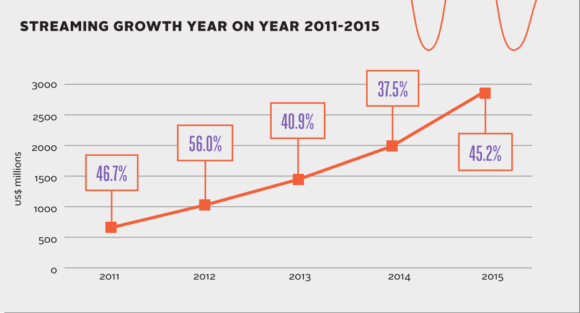
\includegraphics[width=0.7\textwidth, natwidth=580bp, natheight=313bp]{figures/ifpi_stream_growth.png}
    \caption{IFPI's streaming growth report}
    \label{fig:ifpi-growth-report}
\end{figure}

	Music streaming follows this trend of growth on the latest economical reports. Over the five year period to 2015, the observed revenue from the industry grew four times to US \$2.89 billion as can be seen in Figure \ref{fig:ifpi-growth-report} from the IFPI organisation \citep{ifpi}. The increase in the number of paying subscribers is also of notice, seeing an increase from 8 to 68 millions people over the same period. This new model also helped bring some countries where licensed music market was losing ground to piracy like China and Mexico, and it corresponds to around 20\% of the industry's revenue in the top five markets in the world. 
	
	\section{Spotify and the growing competition}	
	
	\begin{figure}[h]
    \centering
    
\includegraphics[width=0.3\textwidth, natwidth=506bp, natheight=900bp]{figures/spotify_screenshot.png}
    \caption{A screenshot of Spotify's Android app}
    \label{fig:spotify-screenshot}
\end{figure}
		
	Spotify is the top music streaming service globally in terms of number of users, totalling 100 millions of which 50 millions are Premium paid subscriptions \citep{spotifypress}. The content is delivered through applications available on several different operating systems like Windows, macOS and Linux, as well as devices like iOS and Android tablets and smartphones, an example is shown in Figure \ref{fig:spotify-screenshot}. Users may access over 30 millions songs available in its catalog through two methods: a free membership where the client is exposed to advertisement, and a Premium paid subscription with additional features like offline downloads, increased music quality and unlimited number of song skips. Spotify also is well known for its music recommendation subsystems like Discover Weekly and Daily Mix that provides playlists tailored to each user based on their listening history. The service is available in most of Europe, as well as in Australia, New Zealand, most of the Americas and several Asian countries.	
	
	The promise of growth in the area however has attracted well known brands to the dispute like Apple and Google, and their growth, while still not up to par with the top players, has been steady and may be significant in the following years \citep{ifpi}. The market is becoming saturated with competition, and any contender to the top position in the music streaming area must strive to keep its current user base at all costs. The loss of a customer, be it for the competition or not, is called in the industry as \emph{churn} and is commonly seen as a metric that should be minimized in a customer relations framework (CRM) of a service provider. For that goal, an important step is to identify prematurely the candidate churning customers and to leverage actions that may avoid them from leaving, and this is commonly achieved by making use of the wealth of historical information that digital providers have about their users. 
	
\section{Churn prediction}	
	
	\emph{Churn prediction}, the task of identifying the customers who are most prone to abandon the service provider, is an established topic in the literature and has seen a considerable amount of research specially on the mobile telecom industry \citep{Hassouna2015} \citep{Lu2014} \citep{Khan2015}.  Several classical techniques for predicting churn like decision trees and logistic regression have been used on recent work \citep{mahajan2015review}, however most of them make use of user behaviour data at a single point in time, normally the most recent one when the dataset was created. The user is commonly represented by summarizing or aggregating his behavioural feature values over a fixed time window, thus losing any latent sequential information that might be contained in the data set. This is a simplification that eases the burden of training a predictor model since the customer data is commonly high-dimensional and difficult to work with, nonetheless latent attributes, when used properly, have been shown to improve significantly a predictor's performance for industries like mobile telecom \citep{GurAli2014}.
    
    Intuitively one can think that latent factors hidden in the temporal axis of the user behaviour data could yield a better prediction accuracy when comparing to a model which leverage a single and static point in time. For instance, a user that is gradually reducing its consumption of the service over time can be easily thought of a prospect churner. While this intuition is trivial to come up with, we are also interested in learning strong correlations between temporal aspects of the data and the churn rate which are not as clear to the eye. Our hypothesis is that making use of the properties hidden on user behaviour data over time, a churn rate predictor could improve its accuracy greatly when compared to methods which are static on time. \Todo{Add this paragraph somewhere else maybe? It seems strange here}
    
\section{User retention}    
    
A churn rate predictor which can identify possible churners accurately is just a trigger on the user retention process that can span several different stages. One of these stages is to identify what actions can be taken by the service provider as to avoid the user abandoning the service. An important problem to solve beforehand is to identify which features of the data have a strong statistical correlation with the churn rate. With that information, the providers could for example set up automated actions as to influence the value on these features. Learning which are the most important features is also of relevance for the task of choosing what data to use for training the predictor models, since commonly service providers have a vast amount of data about the user but only a fraction of that is of importance for predicting churn: training models with a full dataset will commonly introduce error on the system and take a large amount of computing resources to train.
	
\section{Research Question}	
	
The main research question of this project is:

\begin{itemize}
\item Can recurrent neural networks, more specifically LSTMs, achieve a better classification performance for predicting user churn when compared to current state of the art methods for this task?
\end{itemize}	

An auxiliary research question is:

\begin{itemize}
\item How does different aspects of the data, like the class distribution between churning and retaining users, the amount of historical user behavior information, and different representations for the data influences the accuracy of the predictor models?
\end{itemize}


\section{Sustainability, Ethical and Social Aspects}

The protection of user personal data has reached the spotlight in recent years, mainly through its misuse by companies that detain this kind of information. With the widespread use of mobile devices connected to the Internet 24/7, service providers have at their disposal an immense quantity of customer data as fine grained as his exact geographical location, his purchase behavior in e-stores and more. Users are commonly unaware of how their data is being exploited by providers, the exact definition being hidden in thousands of lines in a software agreement written in an obscure way that even specialists may fail to comprehend. Even if fully understood, the legality of its terms is being questioned by courts of law around the world. To protects its citizen's digital data, the European Union has recently issued a set of laws concerning data privacy that shall be put into practice in May 2018 \citep{eu2017protection}.

The misuse of customer information by companies that sparked these concerns has its fair share of examples in the wild. For instance, Facebook released a controversial study where it manipulated the sentiments of its users by feeding into its client's news feed articles leaning towards a positive and negative sentiment, and analyzing how users responded to that stimulus\citep{kramer2014experimental}. However no user was aware of this manipulation, which could inadvertently lead to tragic outcomes that the experimenters failed to consider. 

Another notorious example came from a contest sponsored by Netflix for researchers who could improve its recommendation algorithm, an event known as "the Netflix Prize" \citep{bennett2007netflix}. The massive dataset containing user behavior information on its video platform, alongside a prize of 1 million dollars for the winning team, gathered the interest of researchers all around the world. However a major class-action suit was filled against the company for failing to anonymize user information properly, with customers claiming that they could be uniquely identified through the released data, with the outcome of Netflix canceling future versions of the contest altogether \citep{wired2010netflix}.

The protection of user privacy is a key component in Spotify's business model. Being a company primarily data-driven, it is imperative that Spotify can be trusted in the public's eyes as a custodian of customers' data, both for increasing the user satisfaction with the service and also to avoid similar legal processes suffered by other companies that might deter it from its main mission and priorities. With that in mind, every user personal information is scrambled through a hashing algorithm that makes it impossible to decrypt without the use of the encryption key. If the user ever requests his data to be erased, the removal of this key from Spotify's database makes it impossible for the data to be read and exploited in any way. More so, every non-critical dataset has by default an expiration date on its rows no longer than 90 days, which ensures that data will not live forever in the database.

The computing resources utilized in this project were provided mainly by Google's Cloud Platform data centers. These clusters of machines were heavily optimized throughout the years as to efficiently make use of energy resources, in a way that most companies are incapable of sue to technology and budget constraints. A recent announcement revealed that in 2017 every data centers owned by Google will run on 100\% renewable energy, which is a feat that few other companies can claim \citep{google2017renew}.  


\section{Contributions}

The main contributions of this project can be listed as:

\begin{itemize}
\item Evaluating the performance of a novel recurrent neural network method compared to the standard techniques currently in use for churn prediction.
\item Assessing the impact in accuracy of the predictor models when trained with different quantities of user data.
\item Analyzing how different threshold levels for determining if a user has churned or not affects the performance of classifiers.
\item Experimenting on changing the ratio between the retained and churning classes, and the impact in accuracy that it yields.
\item Evaluating if a more compact representation of user data can improve the performance of predictor models.
\end{itemize}

\section{Outline}

This thesis is organized as follows... \Todo{Write the Outline}

\chapter{Background}

For a better understanding of this degree project, some concepts are required to be properly introduced. Some of them like the ones present in the Definitions section are mainly application-specific, while others pertains to our choice of methodology and evaluation metrics.

\section{Definitions}
\label{sec:definitions}

Every service provider has a different definition of what churn is. Some of them use the explicit cancellation of a contract as a indicator of user abandonment, which has  the advantage of being straightforward to calculate and having a clear correlation to revenue metrics, while others prefer to explore the user activity instead, which has the benefit of better leveraging his satisfaction level and working with the assumption that a satisfied customer has a lower chance of leaving the service for the competition. 

In this degree project, the \emph{user activity} will be used as indication of churn. Even though Spotify has a paid Premium version that could be used as a source of churn labels, a considerable fraction of Free users who generates revenue through advertisement would be excluded from this study. Thus their engagement will be measured instead disregarding for labeling purposes whether they are paying customers or not, however they may be split into different clusters for visualization purposes.

To build up the exact definition of what churn is for Spotify, some concepts need to firstly be introduced, which follows.

\newtheorem{definition}{Definition}

\begin{definition}
The action of a user listening to a song through any of the provider's supported platforms is called a \emph{stream}, also sometimes called \emph{playback}. A stream is initiated when the user starts listening to a song (either by explicitly selecting it through the application or passively by being the next song in a list), and the stream ends when the user listen to a song until it finishes, when he actively skips it by the press of a button, or other technical reasons.
\end{definition}

The playback is the basic measurement of activity of the user on the service. It incorporates the user music streaming behavior, and it is also source of key metrics for the company's financial health. Since Spotify is mainly interested in evaluating the user based on its main feature of content streaming, other user interactions (eg. following another user or artist) are out of the scope for this project. 

\begin{definition}
A user is considered to be \emph{active} during a time period if he possesses one or more streams of at least 30 seconds in length, and \emph{inactive} otherwise.
\end{definition}

The definition of an active user will be important during the sampling phase: there is no interesting information that can be gathered from customers that churned a long time before the first day of behaviour observation. More details about the sampling process will be thoroughly explored in \autoref{sec:sampling}.

Before we arrive in the definition of churn, a brief introduction to time windows will be given to understand further concepts in this section. These definitions will be thoroughly explored on \autoref{sec:timewindows}.

\begin{definition}
The \emph{observation window} is the time span used to observe user behavior and to train the predictor models. It is always followed by the \emph{prediction window} which is exclusively used to predict whether a user in the observation window is going to churn in the future or not. The last few time steps of the observation period is called \emph{activity window}, and is mainly used for fetching user samples.
\end{definition}

\begin{definition}
\label{def:churn}
A user is defined to have \emph{churned} if he is active during the activity window and inactive during the prediction window, and as \emph{retained} otherwise.
\end{definition}

Note that as mentioned before this definition is not concerned whether the user is a paying customer or not, but only if he is actually making use of the service. For example, a user may be subscribed to a Premium paid account and still be considered to have churned if no activity was registered in the prediction window. However, it should be noted that empirical observations by the service provider suggest that there is a significant behavioral difference between the two classes of users that will be taken into consideration when the experiments are performed. 

\section{Time Series and Aggregated Data}
\label{sec:timewindows}

In this section we introduce some concepts that explores the sequential nature of user data. Consider $\mathbf{x}_{nt}$ as the $D$-dimensional vector representing the features of user $n=1,...,N$ at time step $t = t_0,...,t_{\alpha+\beta}$, with $t$ being an equally spaced and discrete time interval. Now consider that the intervals are split into two sequential and non-overlapping time windows: an \emph{observation window} where $t = t_0,...,t_\alpha$ which is going to be used for observing user behavior, and a \emph{prediction window} where $t = t_{\alpha+1},...,t_{\alpha+\beta}$ used solely for predicting whether the user is going to churn in the future or not, with $\alpha$ and $\beta$ being the size of each of the respective windows. A third \emph{activity window} where $t=t_{\alpha-\gamma},...,t_\alpha$ overlaps with the last $\gamma$ time steps of the observation window and it is used for sampling active users. The time windows can be better seen in \autoref{fig:timewindows}.

\begin{figure}[h]
    \centering
    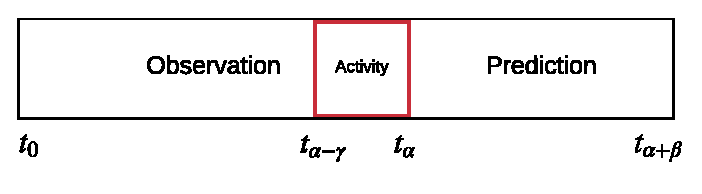
\includegraphics[width=0.7\textwidth,keepaspectratio]{figures/timewindows.pdf}
    \caption{The time windows}
    \label{fig:timewindows}
\end{figure}

Being $\mathbf{x}_n$ a sampled user who is active in the activity window, $y_{n}$ is the variable specifying if customer $n$ has churned between time steps $t_{\alpha+1}$ and $t_{\alpha+\beta}$ of the prediction window, such as

\begin{equation}
y_n = \\ 
\begin{cases}
  \text{0 if user $n$ is active between $t_{\alpha+1}$ and $t_{\alpha+\beta}$} \\    
  \text{1 otherwise}    
\end{cases}
\end{equation}

which assigns one label per customer in our dataset. This definition follows business metrics originated from the service provider, where the counting of active users over a predetermined time span is one of the key metrics indicating business health. For instance, choosing a $\beta$ sized at the number of time periods over 30 days would yield whether the customer will be a monthly active user the following month after being observed for $\alpha$ time steps. 

The literature on churn prediction commonly describes the user features as a single point over the whole observation period, ignoring the time component of the data by transforming it through an aggregation function like the mean. As to train our non-sequential predictor models, we need a similar representation of the data which summarizes all information that we posses of a user over time into a single $D$-dimensional vector. Following the works by \citep{GurAli2014}, we define a \emph{single period training data (SPTD)} as the dataset consisting of one observation per customer who is active during the sampling period. In this approach, the dataset is 

\begin{equation}
\text{SPTD} = [\mathbf{X}_{t_0 \rightarrow t_\alpha}, \mathbf{y}]
\end{equation}

where $\mathbf{X}_{t_0\rightarrow t_\alpha}$ is a $N \times D$ matrix consisting of the constructed features $f(\mathbf{X})$, $f()$ is a feature aggregation function that maps all $\alpha$ user vectors over the observation window to a single one with the same number of $D$ features, and  $\mathbf{X}$ as the $N \times \alpha \times D$ matrix containing information about all users over the whole observation period. $\mathbf{y}$ is a $1 \times N$ column vector containing churn labels for all samples. 

While the simple format of SPTD can be used for training most types of predictor models, it is unsuitable when the goal is to leverage the properties of the time component of the data since it is destroyed after the aggregation function. Thus, we define a \emph{multiple period training data (MPTD)} as

\begin{equation}
\text{MPTD} = \\
\left [  
  \begin{tabular}{c c}
   $\mathbf{X}_{t_0}$   & \multirow{4}{*}{y} \\
   $\mathbf{X}_{t_1}$ \\
   ... \\
  $\mathbf{X}_{t_\alpha}$ \\
  \end{tabular}
\right ]
= [\mathbf{X}, \mathbf{y}]
\end{equation}

which contains a single representation of a user at each time step during the observation period.

\section{Predictor Models}

\subsection{Logistic Regression}

Logistic regression is a linear regression model used to predict the probability of occurrence of a categorical variable, like the churning and non-churning labels. First developed by mathematician David Cox \citep{cox1958regression}, this technique has been used in wide range of domains like medical fields, marketing and economics \Todo{add refs}, and is as of today one of the most used models for predicting the churn rate of customers on the telecom industry \citep{mahajan2015review}. Despite its name, logistic regression is used mostly as a classification algorithm, since its output is a probability score that together with a threshold can map the input to one of the supplied labels (churn and no-churn, for example).

The premise of logistic regression is that the output variable $y$ can be modeled as a linear probability function dependent on a set of input feature values  $\mathbf{x} = [x_1, x_2, ..., x_n]$ through a set of equations that follows:

\begin{equation}
p(y = 1|\mathbf{x}) = f(t)
\end{equation}

\begin{equation}
f(t) = \frac{1}{(1+e^{-t})}
\end{equation}

\begin{equation}
t = w_0 + w_1x_1 + ... + w_nx_n = \mathbf{w}^T\mathbf{x}
\end{equation}

where $y$ is the true output variable that can take the values 0 or 1 in a binary classification problem. $t$ is a linear combination of the input $\bm{x}$ with a trainable weight vector $\mathbf{w}$. $f(t)$ is the logistic function that gives name to the model. This function has the property of "squashing" any real input to a value between 0 and 1, and thus it can be interpreted as a probability. \Todo{Add logistic function}

The likelihood of the logistic regression function can be written as follows:

\begin{equation}
p(\mathbf{y}|\mathbf{w}) = \prod_{i=1}^{n}  p(y_i=1|\mathbf{x})^{y_i} (1-p(y_i=1|\mathbf{x}))^{1-y_i}
\end{equation}

An error function can be usually be defined by taking the negative logarithm of the likelihood function, which follows:

\begin{equation}
E(\mathbf{w}) = -\ln p(\mathbf{y}|\mathbf{w}) = - \sum_{i=0}^{n} y_i \ln p(y_i=1|\mathbf{w}) + (1-y_i) \ln (1 - p(y_i=1|\mathbf{w}))
\end{equation}

Thus, we can pose logistic regression as an optimization problem where the goal is to minimize the error function $E(\mathbf{w})$ 

\begin{equation}
\displaystyle{\min_w} E(\mathbf{w}) + R(\mathbf{w})
\end{equation}

where $R(\mathbf{w})$ is a regularization term, commonly either L1 or L2 norms.

\subsection{Decision Trees}
Decision trees are a class of learning algorithms where the prediction is accomplished by dividing the input space into a series of cuboid regions and then assigning a label (for example "retained" and "churned" for a classification problem) into each one of them. Although simple in nature, it is a widely used method in the in academia, also present in several different papers on churn prediction \citep{Pudipeddi2014}\citep{Hassouna2015} \citep{Ballings2012} \citep{Khan2015}. While there are several different frameworks for implementing a decision tree, this project will focus on the \emph{classification and regression trees (CART)} popularized by Breiman \emph{et al.} \citep{breiman1984classification}. \autoref{fig:dectree} shows an example a decision tree splitting a 2-dimensional input space.  

\begin{figure}[h]
    \centering
    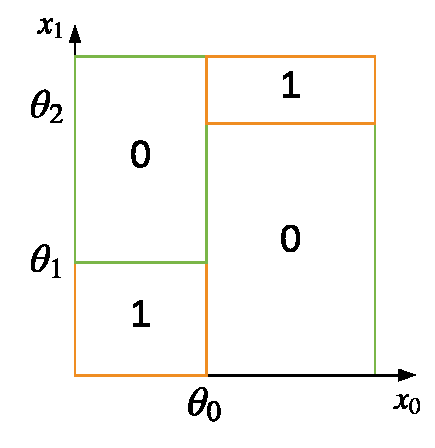
\includegraphics[width=0.5\textwidth,keepaspectratio]{figures/dectree.pdf}
    \caption{Visualization of a 2-dimensional input space being partitioned into 4 regions by a decision tree with its assigned binary labels in each region}
    \label{fig:dectree}
\end{figure}

In this example, the first partition divides the input space into two regions by verifying whether the value for attribute $x_0$ is smaller or greater than $\theta_0$, being $\theta_0$ a parameter learned by the model during training. These two regions are independent after splitting, and thus can be further divided efficiently in parallel. For instance, the region $x_0 <= \theta_0$ is partitioned by comparing if the value of $x_1$ is smaller or greater than $\theta_1$, and since there are no more partitions in this subregion the labels can be assigned. The process is similarly repeated for the region  $x_0 > \theta_0$, where $\theta_2$ was chosen as the splitting point for attribute $x_1$.
 
After the model is trained, it can be easily visualized as a binary tree where each partition corresponds to a node in the tree, and where the leaves contains the identifying labels, which can be seen in \autoref{fig:dectree_bin}. Whenever a new input vector $\mathbf{x}$ is fed to the model, traversing the tree starting from its root will yield a class label in one of its leaves by sequentially navigating through the set of if-else clauses contained at each one of the nodes.  
 
\begin{figure}[h]
    \centering
    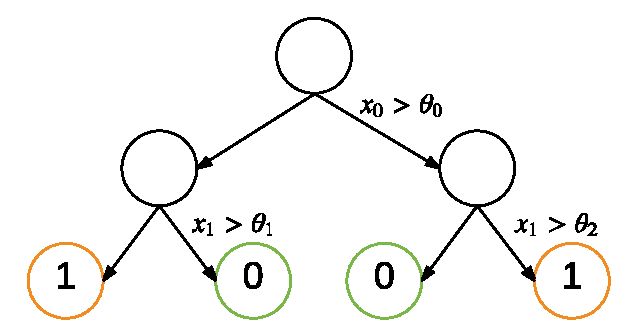
\includegraphics[width=0.6\textwidth,keepaspectratio]{figures/dectree_bin.pdf}
    \caption{Resulting binary tree corresponding to the partitioning performed in \autoref{fig:dectree}}
    \label{fig:dectree_bin}
\end{figure}
 
The learning process of a decision tree corresponds to constructing a binary tree that minimizes the misclassification rate of its training data. That includes finding the optimal number of splits which will define the structure of the tree, and also the values for the splitting coefficients $\theta_i$. To understand how such a tree can be learned, consider a classification problem where $\mathbf{x}$ is a $D$-dimensional vector and $y$ its corresponding class label. The training data is composed of $N$ user vectors forming the $N \times D$ matrix $\mathbf{X} = \{\mathbf{x}_0, \mathbf{x}_1, ..., \mathbf{x}_N,\}$. A tree can be grown by starting at its root and adding nodes sequentially, greedily selecting an attribute and a value to partition the data that minimizes a predefined error function $H(\mathbf{X})$, which can be performed through an exhaustive search. The set of leaf nodes indexed by $\tau$ represent regions $\mathcal{R}_\tau$ where the prediction labels are assigned.

When decision trees are used for classification, a popular cost function is the \emph{Gini coefficient}, a metric commonly used to measure the statistical dispersion of a population. Let $N_\tau$ be the total number of data points assigned to region $\mathcal{R}_\tau$,  the proportion $p_{\tau k}$ of data points in region $\mathcal{R}_\tau$ assigned to class $k = 0,...,K-1$ such as 

\begin{equation}
p_{\tau k} = \frac{1}{N_\tau} \sum_{\mathbf{x}_n \in \mathcal{R}_\tau} \mathcal{I}(y_n = k)
\end{equation}
 
 where $\mathcal{I}$ is the indicator function. The Gini coefficient can be defined as 
 
 \begin{equation}
 H(\mathbf{X}) = \sum_{k=0}^{K-1} p_{\tau k} (1-p_{\tau k})
 \end{equation}
 
which is minimized whether $p_{\tau k}=0$ or $p_{\tau k}=1$. The Gini coefficient favors grouping high proportions of data points that belong to a single class into each region. The splits are chosen to be the ones that minimize $H(\mathbf{X})$ at each node of the tree, which is why decision trees are considered "greedy" algorithms. The tree can be grown until the reduction of the associated error falls below a predetermined threshold. Empirical observations have shown that pruning back some nodes of the tree after the expansion has finished can improve the performance of the predictor.
 
The decision tree algorithm posses a key property which is one of the reasons why it is so popular: the model can be easily interpreted. The ability to visualize the decision process of the predictor model as a binary tree linked together by a simple set of rules is of great value, and is sometimes deemed crucial in fields like medical science for example. However its largest drawback lies in the fact that decision trees are commonly tightly fitted to the data which they were trained on, and small changes in the input may yield radically different models. This problem, which is known in machine learning as high \emph{variance}, is one the reasons for the creation of the ensemble method in the following section.
 
\subsection{Random Forests}

Random forest is an algorithm mainly used for classification and regression which utilizes an ensemble method for prediction: by training several different and independent classifiers, the predicted class or value can be interpreted as the resulting majority vote from all learners, through a mode or mean function for classification and regression, respectively.

Popularized by Breiman \citep{breiman2001random}, random forests have been used in several different domains, specially for the task of predicting user churn \citep{coussement2013customer} \citep{burez2008separating}. The main principle behind the method is that a group of "weak" learners can achieve a better performance when compared to a single "strong" learner, which can also be interpreted as an implementation of the "wisdow of the crowd". 

In this context, a "weak" learner is a decision tree trained with a subset of the samples and features of the original data. No single tree has access to all input variables, however they predict by casting votes on a class, and the final prediction is the class label which has the majority of the votes.

Each one of the trees is grown as follows:

\begin{enumerate}
\item For a dataset of size $N$, sample $N$ examples from the original dataset with replacement, also known as \emph{bootstraping}.
\item For a dataset containing $M$ features, select $m<<M$ which are the number of features selected at random for building each tree.
\item Grow every tree to its maximum extent, without any pruning.
\end{enumerate}

Suppose that we generate $M$ bootstrap data sets and use each one to train a decision tree $y_m(\mathbf{x})$ where $m=1,...,M$. For a classification problem, $y_m(\mathbf{x})$ outputs the most likely class label $k$, that is the highest $p(k|\mathbf{x})$, for every $k=1,...,K$. The final prediction of the ensemble can be defined as the majority vote of every classifier which is given by

\begin{equation}
y_\textit{RF}(\mathbf{x}) = \underset{k \in K}{\arg\max} \{y_m(\mathbf{x})\}
\end{equation}

\subsection{Recurrent Neural Networks}

Recurrent neural networks (RNNs) are a class of artificial neural networks well suited for dealing with data which is sequential in nature. Traditional feed-forward neural networks assume that all input data points are independent of each other, however this can lead to spurious results if this assumption does not hold. For instance, predicting the next word in a text document is tightly correlated with the words that appeared before it. 

Unlike feed-forward neural networks, RNNs allows connections between hidden units, more specifically between the units that are contiguous in time. Updates in a hidden unit in a time step depends on the values in the hidden unit immediately before, and so on until the start of the sequence. While this seems to be a trivial modification over the classical multilayer perceptron, an important property is obtained in the process: RNNs can in theory map the entire history of previous inputs to each output. 

The memory structure that holds this historical data, hereby called \emph{state}, is the main engine that gives RNNs its predictive power. Consider $\mathbf{h}_t$ and $\mathbf{x}_t$ as the values of the state and input at time step $t$, respectively. The value of state $\mathbf{h}_t$ depends both on the current input $\mathbf{x}_t$ and also the previous state $\mathbf{h}_{t-1}$ as follows:

\begin{equation}
\mathbf{h}_t = \sigma(\mathbf{W}^{xh}\mathbf{x}_t + \mathbf{W}^{hh}\mathbf{h}_{t-1} + \mathbf{b}_h)
\end{equation}

where $\mathbf{W}^{xh}$ is the weight matrix connecting the input to the hidden units, $\mathbf{W}^{hh}$ the weights connecting states time steps $t$ and $t-1$, $b_h$ the bias vector for hidden unit $h$, and $\sigma()$ the activation function, commonly the sigmoid or the hyperbolic tangent. Values for state $h_{t-1}$ can be calculated in a similar fashion, until the initial state $h_0$ which is only dependent on the input. This recursive dependence means that an RNN can be "unrolled" through time as to better visualize the interactions between units of the network, which can be seen in \autoref{fig:rnn}.

\begin{figure}[h]
    \centering
    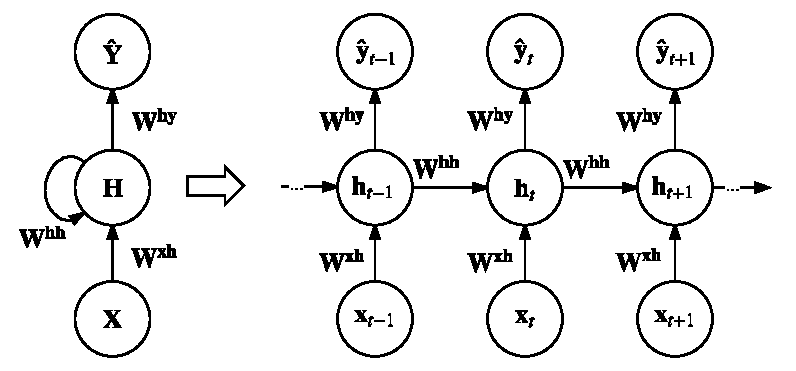
\includegraphics[width=0.7\textwidth,keepaspectratio]{figures/rnn.pdf}
    \caption{A recurrent neural network unfolded through time}
    \label{fig:rnn}
\end{figure}

In a classification problem, the predicted output $\hat{\mathbf{y}_t}$ is a $K$-dimensional vector with the normalized probabilities of input $\mathbf{x}_t$ belonging to the classes $k=1,...,K$, which can be calculated through the following equation:

\begin{equation}
\hat{\mathbf{y}_t} = \phi(\mathbf{W}^{hy}\mathbf{h}_t + b_y)
\end{equation}

where $\mathbf{W}^{hy}$ are the weights connecting the hidden layer to the output, $\phi()$ the softmax function that normalizes its input into probability values, and $b_y$ the bias vector for the output layer. 

\subsubsection{Loss function}

To calculate how effective our prediction is comparing to true labels of the training data, a loss function $\mathcal{L}()$ that computes the distance between true values and the prediction is needed. A common function for a discrete classification problem is \emph{cross entropy} which calculates the amount of information needed to distinguish one distribution from the other, here the predictions $\hat{\mathbf{y}}$ and the true labels $\mathbf{y}$. The equation follows:

\begin{equation}
\mathcal{L}(\hat{\mathbf{Y}}, \mathbf{Y}) = - \sum_k \mathbf{y}_k \log \hat{\mathbf{y}}_k
\end{equation}

\subsubsection{Initializers}

Any neural network requires a method to initialize its weight matrices $\mathbf{W}$. A common practice is set it to small random numbers centered around zero so the weights can independently learn patterns from the data, which is a better approach when compared to naively setting all values to zero. 

Glorot and Bengio\citep{glorot2010understanding} proposed a method to initialize the weights which has widely adopted in academia, and it goes by the name of \emph{Xavier initialization}. In this method, the values are sampled from a uniform distribution such as

\begin{equation}
\mathbf{W} = \mathit{U}[-\frac{\sqrt{6}}{\sqrt{n_\text{in}+n_\text{out}}}, \frac{\sqrt{6}}{\sqrt{n_\text{in}+n_\text{out}}}] 
\end{equation}

where $n_\text{in}, n_\text{out}$ is the size of input and output layers, respectively. 

Another method to initialize the weights was proposed by Saxe \emph{et al.}\citep{saxe2013exact} by choosing $\mathbf{W}$ to be a random orthogonal matrix such as 

\begin{equation}
\mathbf{W}^T\mathbf{W} = \mathbf{I}
\end{equation}

where $\mathbf{I}$ is the identity matrix. This is called \emph{orthogonal initialization}, and it is a commonly used method for initializing the weights of the recurrent state in a recurrent neural network.

\subsubsection{Regularizers}

A machine learning model is judged to be of good quality if it can generalize well to unseen data. When a model shows good performance during training but fails to achieve the same using test data, the model may have fit all its parameters perfectly to the training set instead of finding a function that explains the data well, a problem which is called \emph{overfitting}. 

A common approach to avoid this complication is to add a term in the loss function that penalizes large values of parameters, which is called \emph{weight decay}. This method favors simplicity by avoiding models that overly complex, which can be considered an application of Occam's razor which states that "among competing hypotheses, the one with the fewest assumptions should be selected". A $L_2$-norm is a regularization that penalizes the parameters by adding the square of the magnitude of the weights to the loss function that we aim to minimize\citep{phaisangittisagul2016analysis}, as follows:

\begin{equation}
\mathcal{L}_r(\hat{\mathbf{Y}}, \mathbf{Y}) = \mathcal{L}(\hat{\mathbf{Y}}, \mathbf{Y}) + \lambda \sum_i |w_i|^2
\end{equation}
 
where $i$ iterates over all available parameters and $\lambda$ controls the fraction of the regularization term that will be added to the loss function.

Another common approach is \emph{dropout}\citep{srivastava2014dropout}, which randomly drop hidden units along their connections during training. This technique acts as a regularization method by removing the units with a probability $p$, avoiding the weights of co-adapting too much. Recurrent neural networks however requires a special implementation of dropout as for it be effective, a topic fully explored by Zaremba and Sutskever\citep{zaremba2014recurrent}.

\subsubsection{Optimizers}

The learning process in an RNN involves finding the set of parameters $\mathbf{W}$ that minimizes the loss function $\mathcal{L}()$. This is accomplished by an \emph{optimizer}, an algorithm that iteratively applies small updates to the weights in the direction where loss function is minimal. A classic optimization algorithm is \emph{gradient descent}, which updates the parameters by computing the gradient of the cost function w.r.t the weights for the entire dataset and moving it in the opposite direction, such as

\begin{equation}
\mathbf{W} = \mathbf{W} - \eta \nabla_W \mathcal{L}(\mathbf{W}) 
\end{equation}

where $\eta$ is the learning rate that controls how much of the gradient will be applied to the weights and $\nabla_W \mathcal{L}$ the gradients. Reading the whole dataset to apply one update to the weights is commonly not feasible due to its computing resources requirements. A more popular approach is to apply updates by looking at a subset of the training samples instead, a process  called \emph{mini-batch gradient descent}.

\begin{equation}
\mathbf{W} = \mathbf{W} - \eta \nabla_W \mathcal{L}(\mathbf{W}; \mathbf{x}^{(i:i+n)},\mathbf{y}^{(i:i+n)}) 
\end{equation}

While mini-batch gradient descent is suitable when the dataset is too large to fit into the memory of a single machine, it has its own set of challenges to solve. First, choosing a proper value for the learning rate might be difficult: low values slows down greatly the convergence process, while large values makes the loss function fluctuate around the local minimum and sometimes even diverging from it. Also, a single learning rate regulates the updates of all parameters, not taking into consideration how sparse the data is and how frequent the features are. It is intuitive to think that weights applied to features that rarely ever are different than zero could have a larger update than the ones that are present in every sample.

To address these problems, new optimizers have been recently introduced. \emph{Adagrad} \citep{duchi2011adaptive} is a gradient-based optimization algorithm that adapts the learning rate dynamically based on the frequency of the parameters. Instead of having a single global learning rate, Adagrad instead has a different learning rate for every parameter of the model, making it suitable for datasets that are sparse in nature. Adagrad updates the learning rate for every weight $w_i$ at time step $t$ by looking into the previous gradients that have been calculated for it, as follows

\begin{equation}
w_{i,t} = w_{i,t-1} - \frac{\eta}{\sqrt{\mathbf{G}_{ii, t-1} + \epsilon}} \nabla_w \mathcal{L}(w_{i,t-1})
\end{equation}

where $\mathbf{G}_{t-1}$ is a diagonal matrix containing the sum of squares of the gradients for parameter $w_i$ up until time step $t-1$, and $\epsilon$ a smoothing parameter.

Another optimization algorithm that aims to smartly adjust the learning rate based on the parameters is called \emph{Adadelta}\citep{zeiler2012adadelta}, which is an extension of Adagrad that more efficiently makes use of the stored past gradients. Instead of storing every gradient into matrix $\mathbf{G}$, a fixed sized time window is set, which is used alongside a decaying average function over the past squared gradients in the window, such as

\begin{equation}
\begin{aligned}
\mathbf{E}[g^2]_t &= \gamma \mathbf{E}[g^2]_{t-1} + (1-\gamma)g^2_t\\
w_{i,t} &= w_{i,t-1} - \frac{\eta}{\sqrt{\mathbf{E}[g^2]_t + \epsilon}} \nabla_w \mathcal{L}(w_{i,t-1}) \\
\end{aligned}
\end{equation}

where the running average $\mathbf{E}[g^2]_t$ depends on a fraction of the previous average and the current gradients. A similar unpublished approach that was developed independently and presented in a Coursera lecture by Hinton is \emph{RMSProp}\citep{hinton2012rmsprop}, which will also be used in this project. 

But how are the gradients calculated in a recurrent neural network? This is accomplished through the \emph{backpropagation through time} (BPTT) algorithm introduced by Werbos \citep{werbos1990backpropagation}. The method is an extension of the standard backpropagation algorithm of feed-forward neural networks, where the gradient calculated at time step $t$ is propagated back to the previous time steps until the start of the sequence $t_0$. The reader is invited to refer to Werbos' paper for details of its implementation.

\subsubsection{Vanishing and exploding gradients}

Even though theoretically RNNs can be used to map input and output sequences of an arbitrary size, in practice learning from long-range dependencies poses a challenge that is difficult to overcome. This is due to a problem called \emph{vanishing and exploding gradients} explored by Bengio \emph{et al.} \citep{bengio1994learning} and extended by Hochreiter \emph{et al.} \citep{hochreiter2001gradient}. Neural networks learn by updating the parameters by a proportion of the gradient of the error function w.r.t the current weights, and this process can be made difficult either if the gradients go to zero (no learning at all) or explode to large numbers (missing the local optima at every turn). In RNNs and also other deep architectures, the top layers may fail to learn in an adequate pace since its update is backpropagated through the bottom layers by multiplying the intermediate gradients through the \emph{chain rule}. If those gradients are consistently between -1 and 1, which is the case of the most common activation functions, through the chained multiplication of the derivatives the weight update of previous layers will quickly approach zero. Other activation functions like the Rectified Linear Unit $max(0,x)$ may instead make the gradients increase rapidly due to its constant derivative of 1 w.r.t $x$ for every value greater than 0.

Some solutions have been proposed to tackle this complication. A well-known variant of the learning algorithm of RNNs is the \emph{truncated backpropagation through time} (TBPTT) which aims to solve the exploding gradient problem for continuously running networks \citep{williams1989learning}. In it, one can set a maximum number of time steps alongside which error can be propagated. Using a small cutoff value would alleviate the problem of gradients increasing too fast, however at the cost of learning long-range dependencies. A more modern approach however carefully design the nodes as to avoid the vanishing and exploding gradients problem while also being able to learn from information hidden long back in the input sequence, which shall be explored in the following section.

\subsection{Long Short-Term Memory}

The Long short-term memory network is an extension of a RNN that can extract long-range dependencies from the sequential input without suffering from the negative consequence of the vanishing and exploding gradients common in deep architectures. Firstly proposed by Hochreiter and Schmidhuber \citep{hochreiter1997long} and further extended by Gers and Schmidhuber \citep{gers1999learning}, this technique has recently been applied successfully for domains like speech recognition \citep{graves2013speech} and video classification \citep{yue2015beyond}.

The main property that differentiates LSTMs with its classic counterpart is its \emph{memory cell} which controls the flow of information that goes from the input $\mathbf{x}_t$ to the hidden states $\mathbf{h}_t$. This is accomplished by using a unique \emph{cell state} variable $\mathbf{s}_t$ which contains the global information that the network currently has about the input sequence, which can be seen as its "memory". A visualization of the memory cell and its traversing state variable can be seen in \autoref{fig:lstm}.

\begin{figure}[h]
    \centering
    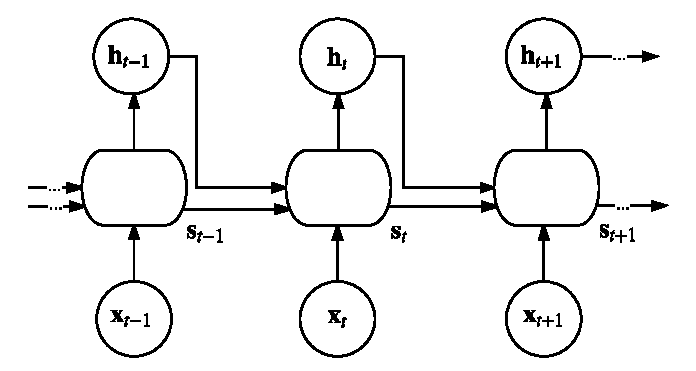
\includegraphics[width=0.7\textwidth,keepaspectratio]{figures/lstm.pdf}
    \caption{A LSTM network unfolded through time, with the oval shaped structure as the memory cell}
    \label{fig:lstm}
\end{figure}

The memory cell structure of a LSTM is responsible for updating the cell state at each time step. This is accomplished by a set of so called \emph{gates} that controls how the information will get in and out of the cell state. A modern LSTM architecture is composed of three of these gates, hereby called \emph{input}, \emph{output} and \emph{forget gates}, alongside the \emph{input node} which is a transformation over the raw input sequence. A LSTM memory cell at time step $t$ is fully described by the following set of equations:

\begin{equation}
\begin{aligned} 
\mathbf{g}_t &= \sigma_g(\mathbf{W}^{xg}\mathbf{x}_t + \mathbf{W}^{gh}\mathbf{h}_{t-1}+\mathbf{b}_g) \\ 
\mathbf{i}_t &= \sigma_i(\mathbf{W}^{xi}\mathbf{x}_t + \mathbf{W}^{ih}\mathbf{h}_{t-1}+\mathbf{b}_i) \\
\mathbf{f}_t &= \sigma_f(\mathbf{W}^{xf}\mathbf{x}_t + \mathbf{W}^{fh}\mathbf{h}_{t-1}+\mathbf{b}_f) \\
\mathbf{o}_t &= \sigma_o(\mathbf{W}^{xo}\mathbf{x}_t + \mathbf{W}^{oh}\mathbf{h}_{t-1}+\mathbf{b}_o) \\
\mathbf{s}_t &= \mathbf{g}_t \odot \mathbf{i}_t + \mathbf{s}_{t-1} \odot \mathbf{f}_t \\
\mathbf{h}_t &=  \sigma_h(\mathbf{s}_t) \odot \mathbf{o}_t
\end{aligned}
\end{equation}

where $\mathbf{i}_t, \mathbf{o}_t, \mathbf{f}_t$ are the input, output and forget gates, respectively. $\mathbf{x}_t, \mathbf{h}_{t-1}, \mathbf{s}_{t-1}$ are the input vector at the current time, and the hidden units and cell state from the previous time step, which are the inputs to the memory cell. $\mathbf{W}, \mathbf{b}$ are the weight matrices and the bias vectors for each gate and node. $\mathbf{g}_t$ is the input node. $\sigma$ are the activation functions: modern architectures use $\sigma_g,\sigma_h$ as the hyperbolic tangent function, whereas $\sigma_i,\sigma_f,\sigma_o$ as the sigmoid \citep{zaremba2014learning}. The output of the memory cell are the updated cell state $\mathbf{s}_t$ and hidden units $\mathbf{h}_t$.

One can intuitively think of LSTM gates as controllers whether the activation for a given unit is let in and out of the cell state at each time step, which can be learned during network training. During the forward pass, if the input gate is zero, no activation can get into the cell state. Similarly, the output gate learns when it should let the activation leak out of it. The forget gate being equal to zero erases all the memory previously stored on the cell state, basically forgetting what was learned in the past. During the backward pass phase, the gradient may propagate several time steps in the past without exploding or vanishing due to its constant error carousel. Through this angle the memory cell learns as to when it should let the error in and out of the cell state.

Networks that makes use of the memory cell structure of an LSTM have been shown to outperform classical recurrent networks by being able to learn long-term dependencies from the sequence in a more efficient way. Positive results were obtained both in artificial datasets carefully designed to test the ability of the network learning long-term dependencies \citep{bengio1994learning} and more recently in demanding sequence processing tasks \citep{graves2013speech}\citep{sutskever2014sequence}.

\section{Dimensionality Reduction}

\subsection{Principal Component Analysis}

Principal component analysis (PCA) is a widely used method for applications like data compression, dimensionality reduction and data visualization. Initially invented by Pearson\citep{pearson1901liii} and later independently developed and named by Hotelling\citep{hotelling1933analysis}, PCA strives to find an orthogonal projection of the original data into a lower dimensional space (also known as the principal subspace) where the variance of the projected data is maximized.

Consider a dataset composed of $N$ samples, each one being $D$-dimensional vector $\mathbf{x}_n$, and also a $D$-dimensional unit vector $\mathbf{u}$ where the samples are going to be projected on. The goal of PCA is to find a projection into a $M$-dimensional space where $M < D$ and where the variance of the projected observations are maximized, which can better be visualized in \autoref{fig:pca}.

\begin{figure}[h]
    \centering
    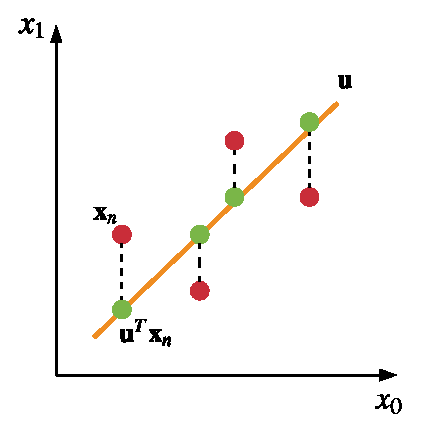
\includegraphics[width=0.5\textwidth,keepaspectratio]{figures/pca.pdf}
    \caption{An example of PCA reducing the dimensionality of the data}
    \label{fig:pca}
\end{figure}

After projecting the observations into the unit vector previously defined and obtaining $\mathbf{u}^T\mathbf{x}_n$, the variance of the projected data can be calculated with the following set of equations:

\begin{equation}
\begin{aligned}
\mu &= \frac{1}{N}\sum_{n=1}^N \mathbf{x}_n \\
\Sigma &= \frac{1}{N}\sum_{n=1}^N (\mathbf{x}_n - \mu)(\mathbf{x}_n - \mu)^T \\
\mathbf{V} &= \frac{1}{N}\sum_{n=1}^N (\mathbf{u}^T\mathbf{x}_n - \mathbf{u}^T\mu) = \mathbf{u}^T\Sigma\mathbf{u}
\end{aligned}
\end{equation}

where $\mu$ and $\Sigma$ are the mean and the covariance matrix of the sampled data, respectively. Maximizing the value of the variance $\mathbf{V}$ with respect to $\mathbf{u}$ is an optimization problem constrained by $\mathbf{u}^T \mathbf{u}=1$. Hotelling\citep{hotelling1933analysis} shows that by introducing a Lagrange multiplier $\lambda$, this can be turned into an unconstrained optimization where

\begin{equation}
\mathbf{u}\Sigma\mathbf{u} = \lambda_1
\end{equation}
	
and so the variance will be maximized by picking the eigenvector corresponding the largest eigenvalue $\lambda_1$, which is known as the first \emph{principal component}. The following $M-1$ principal components can then be chosen sequentially by picking the vector which is orthogonal to all other principal components already considered, which is equivalent to choosing the eigenvectors corresponding to the largest $M-1$ eigenvalues $\lambda_2,..., \lambda_M$.

\chapter{Related Work}

There is considerable amount of work done on the churn prediction realm. The most common topic that is addressed by the literature is evaluating different types of predictor models trained on a domain-specific dataset, like the telecom and financial industries for example. Understanding what techniques are commonly used on the field is deemed crucial for the success of any churn rate predictor model.

The use of data represented as a time-series for predicting churn, although of high interest to this project, is a rather under researched topic as of today, the user features being commonly aggregated over a time window on the whole observation period. Recently though some interest has been sparked on the literature about trying to leverage temporal aspects of the user behaviour by representing the data as a sequential input, and some examples similar to the task at hand, while not abundant, can nevertheless be found. 

Other research papers focus on answering how different properties inherent to the churn prediction problem affect the performance of classifiers, like for example how to deal with unbalanced data sets, how the evaluation procedure should be performed and how far back in the user history should models be trained on as to obtain a proper balance between accuracy and processor usage.  

This chapter will introduce the literature on the fields of interest for this project, and will focus mainly on the following topics:

\begin{itemize}
\item Identifying the state-of-the-art for training, modeling and evaluating churn predictor classifiers, the algorithms being used, the methodology for the experiments and the observed results.

\item Researching current techniques for creating models that leverage the properties of time-series data, applied for churn prediction (if any) or similar domains where we can map our problem to. It shall also be studied common features of sequential data as to better understand how to best exploit its properties as to improve the accuracy of our models.

\item Understanding prevalent characteristics on data sets used for churn prediction as to improve the performance of models and also to avoid common pitfalls when training and evaluating their accuracy.
 
\end{itemize}


\section{Churn Prediction}

Identifying which users are most likely to churn is an important step in any customer relationship management (CRM) framework interested in improving user retention. It has been shown that several economical values are directly correlated with the customer lifetime metric that can be crucial in a competitive market, like how the costs of acquiring new customers surpass those of retaining existing ones and how loyal users usually spend more and can bring in new customers \citep{GurAli2014}. Thus, churn rate prediction is an established topic in the literature and has seen studies being performed on a wide range of domains like the telecommunication industry \citep{Lu2014}\citep{Khan2015}\citep{Hassouna2015}, social multiplayer games \citep{Borbora2011}\citep{Runge2014} and community-based question answering services (CQA) \citep{Pudipeddi2014}\citep{Dror2012}. 

The very first aspect of the study that any researcher has to take into consideration is the formal definition of what churn is, which depends on the domain that the data set belongs to. \citep{lazarov2007churn} divides the definition into three types: \emph{active} where the contract is officially terminated, \emph{hidden} when the customer is inactive (not using the service) for a significant amount of time, or \emph{partial} when the customer is not using the service at its fullest, opting for a competitor instead. Subscription-based services like mobile companies \citep{Lu2014}\citep{Hassouna2015} and massive multiplayer games \citep{Borbora2011} commonly utilizes the active churning definition caused by the explicit termination of the agreement. Social games \citep{Runge2014}\citep{Drachen2016RapidPO} and CQA services \citep{Pudipeddi2014}\citep{Dror2012} however usually model the user interest by measuring its level of activity and engagement since no contract is formally established, opting for the hidden churn definition instead. 

Even though Spotify has a contract-based Premium service, this project is interested in the clients who are inactive for some time, whether they are paying customers or not. Delving into the hidden churn definition, one could ask what is considered a "significant amount of time" as to judge a user to have churned or not, and different domains have distinct approaches depending on the way the interaction between user and service takes place. For example, for a mobile network like the one studied in \citep{Khan2015} this definition can span months of inactivity since customers on that market are commonly more loyal, even though this paper focus on pre-paid accounts with "soft" contracts. On the other hand, rapid-changing markets like free-to-use services as social games and CQA sites prefer to define the churn period as small as possible (commonly days or weeks), since the absence of an agreement makes it easy for customers to switch for the competition, having the service the obligation to act faster if any sign of loss of users is identified \citep{Khan2015}\citep{Drachen2016RapidPO}. On \citep{Dror2012} the focus is set on new users so the the churn period is explicitly set to be their first week of activity. \citep{Pudipeddi2014} however focus on both new and experienced users by considering the first days and posts (questions and answers) as parameters on the models trained, evaluating each independently.

Current literature for prediction of churn rate uses a wide range of machine learning technologies, such as decision trees \citep{Pudipeddi2014}\citep{Hassouna2015} \citep{Ballings2012} \citep{Khan2015}, logistic regression \citep{GurAli2014}, neural networks \citep{Runge2014} and its convolutional variant \citep{Wangperawong2016}, random forests \citep{Dror2012} and support-vector machines \citep{coussement2008churn}. The number of techniques is vast, however it can be mentioned that current research suffers from a difficulty to reach insights that can generalize well for other areas, since the applications that the data sets belong to are domain-specific, greatly influencing how the users interact with the service. Interpretability is a key component in any application since the end goal is always not only to detect the users most likely to defect but also the reasoning behind their departure, as to plan reasonable actions to increase retention. With that in mind, even though some models like weighted random forests \citep{Burez2009} and neural networks \citep{Runge2014} offer a higher accuracy for some domains, the difficulty in getting key drivers behind the consumer's behaviour in some "black-box" type of models have led to researchers opting for a more interpretable technique like logistic regression which is commonly a close second place in terms of performance \citep{Runge2014} \citep{Dror2012}. For that reason, decision trees and logistic regression are as of today the most popular techniques for churn prediction, yet a consensus of the best model cannot be reached by researchers as stated by \citep{mahajan2015review}. 

The telecom industry is by far the most well researched area for predicting churn, and a proper review would be incomplete without mentioning some examples. In \citep{Hassouna2015}, two popular models for predicting user churn were empirically compared: decision trees and logistic regression. By making use of the data set provided by a mobile operator, two models were created by independently training and selecting their best performing versions. Evaluation was executed by comparing the AUC of their ROC curves, as also their Lift score and overall accuracy. The conclusion is that decision trees consistently perform better when compared to logistic regression models, and thus should be a preferred choice. In \citep{Lu2014}, churn classification was performed on users in a rather unique way. The Gentle AdaBoost boosting algorithm was used alongside a logistic regression base learner as to train a model to do the separation between the churning and non-churning classes. However, one further step was performed where the users were split into two clusters based on the weights assigned by the boosting algorithm. One of the clusters was identified to have a considerably larger churn rate than the other, and thus another logistic model was trained using the clusters as labels, and its performance evaluated using ROC curves. The idea behind this approach is to use a model to mark users who have a high risk of leaving the service (and be the focus of user retention actions), instead of labelling them as churners and non-churners directly. On \citep{Khan2015}, billions of call detail records from a mobile phone operator was the focus of a churn prediction study and feature analysis. The initial data set was filtered to the calls made by 100.000 subscribers during a 6 month period. A brute-force approach to feature engineering was then performed to create 12.914 out of the initial 10 features by combining every feature from each of the manually split 8 different groups. Feature selection is then performed in two distinct ways: first, an individual Student's t-test score is computed for each individual feature to evaluate how well it can differentiate between the churners and non-churners sets. Second, a tree-based method was used as to estimate the the accuracy of a joint classifier by adding features one at a time. Features are then ordered by their statistical correlation with churn, and the top 100 features were selected to train several different classifiers. Evaluation was performed mainly by comparing the AUC of each model, where AdaBoost using a decision tree classifier performed the best, followed closely by a logistic regression model.

The rapid increase in Internet popularity has spawned a plethora of new services in the last decade, and thus a wider range of domains like CQA sites and gaming applications are being researched for churn prediction. In \citep{Dror2012}, an explorative study was made on the Yahoo! answers website as to discover an efficient churn predictor model and also the features that correlates with the user leaving the service, however differently from other works this paper focused on new users with less than a week of activity on the service. Features were grouped into Question, Answer and Gratification categories, and were used for training several different classifiers. For this dataset, random forests performed the best with logistic regression as close second. Features were also ordered by the amount of information gain that they provide, and the number of questions and answers are the top features on that regard (inversely correlating with churn), followed by the period of time the user is active and gratification features for answers given and questions made. In \citep{Pudipeddi2014}, the younger CQA service Stack Overflow was the focus of a study on user behaviour characterization and churn rate prediction. An extensive data exploration was made as to correlate features to the chance of a user leaving a service, and with those insights classical modelling techniques were used, where the best performing one was a decision tree. The approach used for extracting and categorizing features (temporal, frequency, gratitude, etc) and the insights that follow the study (like the importance of temporal features for predicting churn) is of high value and can be mapped to concepts on a different domain like a music streaming service with minor modifications. 
In \citep{Runge2014}, players responsible for generating the most profit on two casual social games were the focus of a study on churn analysis and prediction. Formal definitions for active players and churning were made, and the problem was defined as a binary classification task where users were labelled as leaving the service or not in the following week of when the models were trained. Four different models were then trained, and a neural network classifier obtained the best area under the curve (AUC) score, with logistic regression as a close second. The formal definitions of "churn" and "activity" can be applied to a music streaming service in a similar way, as the evaluation of performance using a series of receiver operating characteristic (ROC) curves. In \citep{Borbora2011}, the activity log of a subscription-based multiplayer online game was the source of an experiment focused on comparing two different methods for predicting the users with a higher tendency to leave the service, a theory-driven and data-driven approaches. For the modelling, an ensemble method was used with several different classifiers, where the choice of model was made based on whether the cluster of the data set (found with K-means) that will be used to train the classifier has a significant proportion of churners or not. Even though the performance of the data-driven model was superior, the difference was negligible when taking into consideration the complexity of the models and also its interpretability. Moreover, if marketing resources are constrained the theory-driven model was considerably superior for the first 40\% of users on the lift chart. 


\section{Sequential Modelling for User Behavior Data}

Even though there is currently a wealth of research on churn prediction techniques, most of them treat the user behavioral features as static points in time by aggregating or summarizing their values over a time window \citep{Auon2015}. It is a simplification that eases the hassle of training models with a data set which is commonly high-dimensional and difficult to work with, however information that could be used to improve the predictors' performance is lost in this process  \citep{GurAli2014}. For example, there is no information as to when over the time window being analyzed a user decides to churn, it could be that all defectors are grouped into a period where an external event (like the end of an offer) has taken place. Environmental variables, that is those that varies through time but are common to all users, are also omitted on static models, leaving it to the experts the task of manually integrating these features on their analyses. Newer models like \citep{Pudipeddi2014} attempt to integrate some temporal data by manually engineering features related to time (like the duration of an event, for example), however since each user is represented as a sample in a single point in time the sequence of data transformations is inherently lost in this process.

It is natural to think that the human behaviour evolves through time. Our opinions and desires changes in accordance to the stimuli that we receive from the world around us, and summarizing our persona by looking at a single point in our life is an oversimplification that does not make justice to the path that leaded us to where we are. Dealing with temporal data is by no means trivial however, and to leverage fully its properties some careful considerations about this type of data must be done. On \citep{Langkvist2014}, an overview of the challenges on creating models that make use of the time component on data sets are presented to the reader. Also, since hand-crafted features are generally domain-specific and difficult to create, a review of the current research on unsupervised feature learning applied for time-series data is the focus of this paper. From the challenges, it is worth of mention the uncertainty that there is enough information to understand the underlying process, its non-stationary characteristics like mean, variance and frequency, and its common high dimensionality and noise. The right representation is deemed then crucial for any model to be successful in its goal. Several different techniques currently being used for unsupervised feature learning are then presented in details to the reader, where it is worth of quick mention the conditional Restricted Boltzmann Machine (cRBM), Recurrent Neural Networks (RNN, with is Long Short-Term Memory extension), the Gated RBM, the Time-Delay Neural Networks, and the Space-Time Deep Belief Network. Finally, several classical time-series problems are reviewed alongside the best models currently being used for each domain. 

The hypothesis that sequential patterns hidden on temporal data can improve the accuracy of predictor models is not an uncharted territory however, and has being recently explored by researchers on similar domains as churn prediction that could be mapped to with minor modifications. Sparked by positive results of recurrent neural networks on domains like speech recognition \citep{graves2013speech} and video classification \citep{yue2015beyond}, some papers attempt to recreate similar deep architectures on their own prediction problems. On \citep{Tax2016}, a technique was presented as to predict the next event and its timestamp on a running case of a business process (a help desk process, for example). Three different LSTM architectures were experimented on, one for each of the problems being tackled: estimating the next activity and its timestamp, all the remaining activities in a use case and the remaining time of a process. This technique could be used for churn prediction by interpreting the user interaction with the service as actions, and "churn" could be an event that may or may not exist in the process chain. The LSTM architecture was also present on \citep{Auon2015} alongside a quantile regression (QR) model as to predict which of the past buyers of a store chain will return after acquiring a product on sale. The hypothesis is that a performance gain can be achieved by combining models that are know to perform well on both temporal and aggregate features, respectively. It was empirically shown that a mixture of experts approach between these two techniques can reach a significant mean-square error improvement when comparing to any of the models when evaluated independently. 

Deep architectures like LSTMs could theoretically be applied in a similar way for the task of predicting which users are more likely to abandon a service, however the lack of research using techniques like these suggests that this mapping may not be as easy as it seems, nevertheless some examples can still be found in the literature. Inspired by results obtained on image recognition \citep{krizhevsky2012imagenet}, a convolutional neural network (CNN) model was used as a churn predictor on the work by \citep{Wangperawong2016}. On it, users were represented as 2-dimensional images where columns are the tracked features and rows are days organized in sequences. Two different CNN models were used, and both outperformed a baseline decision tree model. On \citep{GurAli2014} the researchers propose a new data set generation framework that can better leverage the temporal aspect of user behaviour data for churn prediction models. The hypothesis being tested is that by boosting the data with features on different time periods instead of only the last one, a significant performance gain can be achieved. The main framework of this study is called Multiple Period Training Data (MPTD), which basically consists of aggregating to each user their features at each predefined time step along the time range of the data set, alongside their churn labels at each point in time and also environment variables which varies through time but are common for all users. This framework was tested against a classical static data set, demonstrating a significant improvement (by \emph{p-value} comparison) on AUC and TDL for both logistic regression and decision tree models for predicting if the user is going to churn on the next test period or nor. Another experiment was focused on predicting churn several periods on the future, and for that a common survival analysis method called Cox regression was used as a benchmark for comparison against logistic regression models trained on MPTD. It was empirically concluded that using several independently trained binary classifiers, each trained on a different parameter to the "churn within $\delta$ periods" (W$\delta$C) feature, a significant performance gain can be achieved when comparing their respective AUC and TDL.


\section{Evaluating and Training Churn Prediction Models}

Data sets from service industries often have a common characteristic that may be problematic while training models, which is the uneven distribution between the churning and non-churning classes. It is a common scenario for the number of non-churners to heavily outweigh the number of churning samples on real data sets. Class imbalance is thus a recurrent concern in almost all domains, however research in this area lacks the proper attention. \citep{Burez2009} aims to solve this mystery by focusing entirely on how the uneven class distribution affects the performance of several different classifiers. The performance boost estimated to be received by using a cost-sensitive learning algorithm (where false negatives are assigned a greater cost than false positives) is also evaluated, and it has taken the form of a weighted random forest model which was compared to other classical baseline models like logistic regression and random forests. Under-sampling, where fewer samples from the majority class are incorporated in the training data as to artificially change the distribution between the labels, is proved to significantly improve the performance of the underlying models, however the exact ratio between churners and non-churners is confirmed to be case-dependant, not necessarily being the even distribution the perfect choice. 

To deal with the problems brought by the unbalanced distributions mentioned above, proper evaluation metrics must be used as to avoid the predictors to be biased towards the majority class. It is a well know fact that the accuracy of a classifier is not an appropriate method when comparing the performance of different models \citep{powers2011evaluation}, and so no paper reviewed used this metric by itself. The overwhelming majority of the literature abides by the use of AUC as a proper metric for predicting churn rate, \citep{Ballings2012} \citep{GurAli2014} \citep{Khan2015} \citep{Lu2014} to name a few. \citep{Burez2009} delves into this topic and defends the use of AUC as a proper metric, while adding the cumulative gains chart as to graphically represent the percentage of customers has to be targeted to reach a percentage of churners. The F-score is also sometimes added as a metric of interest, normally in conjunction with AUC \citep{Dror2012} \citep{Khan2015}. In respect to graphical representations, ROC curves and lift charts dominates the literature as appropriate methods, and it is present in works like \citep{Lu2014} and \citep{Burez2009}. 

Another question that can be made is how far in the user history models must be trained on as to achieve the best trade-off between accuracy and computational burden. It is intuitive to imagine that user actions far in the past exerts little influence on predicting whether the user is going to churn or not in the near future, however the exact threshold that should be used is not trivial to find. \citep{Ballings2012} attempts  to answer this question by experimenting with three different models (logistic regression, decision trees with and without bagging) on a newspaper data set consisting of 16 years of user history. The models were evaluated for their performance by training with data ranging on this interval with a 1-year gap between each measurement. It has been concluded that  after year 5 no gain in performance (measured by AUC) is statistically relevant enough to warrant the increase in computational power needed for the training. However, the researchers also question whether this result can be extended for other domains or not, leaving that for future work.

Current data sets from service providers have no lack of user historical information stored, however the probability that all available features have a significant correlation to churn rate is pretty slim. Using too many features may lead to undesirable effects like overfitting and falling into the "curse of dimensionality" problem, reducing the classifiers performance as cited by \citep{guyon2003introduction}. It is a common step to pre process the data in a way as to mitigate this risk, but still there is no single method in the literature that dominates the scene. Several papers do a manual subset selection of features based on theories, testing each using baseline classifiers and selecting the subset with the best performance \citep{Pudipeddi2014}\citep{Runge2014}. Others works like \citep{Borbora2011} and \citep{Dror2012} use information gain as a metric to classify the features on their expected reduction in entropy. One step further is taken by works like \citep{Lu2014} and \citep{Khan2015} where full decision trees are built specifically for feature selection. Another more exotic method was used by \citep{Wangperawong2016} with an autoencoder to discover which features influenced the churn rate the most. 

Churn prediction has been explored in different kind of applications on recent literature, however music streaming services are as of today a quite under-researched area, even though there is a prominent feature that makes it significantly different from other more researched and similar areas like video streaming, which would be the absence of the constant attention factor that video demands. Studying the user behaviour in each application can possibly help optimizing parameters that are difficult to tune without expert knowledge on how the interaction between costumer and application occurs. The work by \citep{Zhang2013} aims to fill that gap by analysing patterns of usage of Spotify's Premium subscribers on features like session and playback arrival patterns, user behavior on single and multiple devices and favorite times of day for streaming. The main contributions of the study can be summarized as follows: First, daily patterns can be observed on features like session arrival, playback arrivals and session length. Second, there is a high probability of users to continue on the same device for consecutive sessions. Third, users have their unique times of day when they prefer to stream music on the platform. Fourth, a session length can be used as a good indicator of the next session length and also downtime.

\chapter{Dataset Creation and Exploration}
\label{chap:dataset}

\epigraph{In God we trust: all others bring data.}{\textit{William Edwards Deming}}

Creating a dataset that is suitable for predicting churn is far from being a trivial task. Spotify has at their disposal an enormous amount of data that tracks every user interaction with the application, reaching terabytes in size every single day. This chapter will be dedicated to delving into details on how the dataset used for training our models was generated, how the sampling was performed, which features were chosen and engineered, and also exploring it in details.

\section{Infrastructure and Data Sources}

Every time a user streams content on Spotify, be it through the mobile application, desktop, web or any other platform, it generates a log entry with information regarding details on what has occurred in this interaction. This information can be the feature of the application used on this stream, its length in miliseconds, the context in the app where this stream originated from, to cite a few. Through a complex data pipeline, all the log data from different clients is aggregated into a massive dataset hosted in a cloud provider, and is externalized through Google's fully-managed query service called BigQuery \citep{sato2012inside}. 

After processing and cleaning procedures, a set of tables, named by the provider as \emph{ReportingEndContent}, are generated one for each day, and it serves as the main source of data for this project. The tables have an average of 2.8 billions of rows with 38 columns, occupying up to 1.7 TB of storage in disk each, one of the largest datasets currently stored in Google Cloud platform. These tables are further joined with other tables as to gather a more detailed information about the stream, which are capped to a limit of 90 days due to privacy rules established by the provider.

\section{Dataset Creation}

Creating a dataset that realistically represents the target population of this is by no mean an easy feat to accomplish. While it is desirable to train models with all the data that is available to us, doing so is an engineering feat by itself that could span the entirety of a project. Thus, we need to make smart decisions as to create a dataset that is representative of the audience while also avoiding scalability pitfalls that eventually occurs when working with big data.

In this section, the \emph{data pipeline} used for building the data used for model training and evaluation will be presented, which can be seen in \autoref{fig:pipeline}. Each subsection corresponds to a sequential stage in the pipeline, while the source are the raw stream information provided by the table \emph{ReportingEndContent} and the output is the dataset in a format suitable for model training.

	\begin{figure}[h]
    \centering
    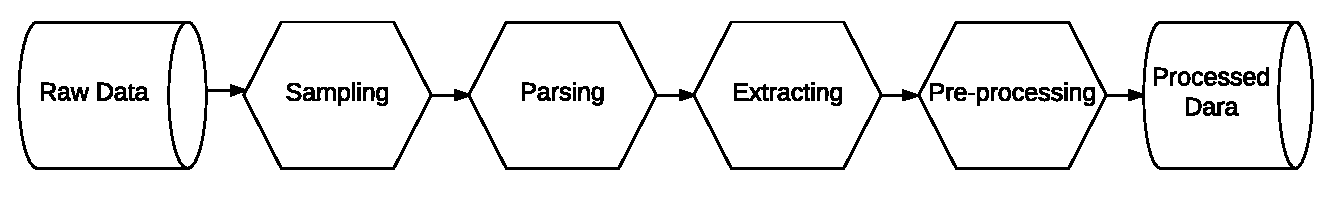
\includegraphics[width=0.9\textwidth,keepaspectratio]{figures/pipeline.pdf}
    \caption{Dataset creation pipeline}
    \label{fig:pipeline}
	\end{figure}

\subsection{Sampling}
\label{sec:sampling}

Each day hundreds of terabytes of streaming information are collected through the provider's data pipelines, aggregating customer usage of the application over several different platforms and countries. Since it is out of the scope of this project to train models with the data in its entirety, one of the challenges will be to understand the information that is available to us and to choose a subset of samples that are representative of the target population that we intend to focus on in this study. This task can be extremely daunting by itself, so this project will make use of previous private studies performed by the service provider as a guidance on which features to choose.

The main rule applied for sampling users is by filtering those who have at least one stream of significant length during the activity window described in \autoref{sec:timewindows}. The minimum length of the stream is set to be 30 seconds, which follows rules of royalty payments from the service provider. By applying this filter, we make sure that the users were active right before the period of prediction. Thus, users marked as churning did so between the period of observation and prediction, and we guarantee that we are not choosing samples who churned a long time ago.

Selecting users that created accounts any time during the observation period might skew our models towards a level of inactivity that does not corresponds to reality. For example, if a new account was created right by the end of the observation window, we might erroneously assume that the user was inactive for all days before the registration date. To avoid this, only users that registered into the service any time before the observation starts are sampled into our dataset. 

Spotify is a service provided to countries all around the world, and we must be aware of the influence that seasonality plays into user behaviour if we intend to avoid overbiasing our samples. To limit the influence of day-night cycles in the learning process, users were sampled from three countries which share a similar timezone between each other and encompass a large share of Spotify's userbase, that is Brazil, Mexico and United States. \Todo{Review the paragraph about countries}

The Spotify service is provided through a wide range of platforms like through Apple's iPhone or a desktop PC. To minimize the influence that different platforms may have on predicting churn, and also due to higher reliability on collected metrics, the dataset shall be filtered on streams performed on the Android platform, be it on a smartphone or tablet device. \Todo{Check Sahar: This is only for sampling, so will this be true?}

Even after all the previously mentioned filters, we are still left with a large amount of users which is more than any single machine could handle. While randomly selecting samples is a common performed method, for reproducibilty reasons we instead choose to deterministically select samples by applying a hash function over the user ID followed by a modulo operator over the desired fraction of users. Through this method we guarantee that the same users will be sampled, as long as the fraction does not change.

Through the application of all aforementioned rules, a grand total if \emph{518.233 users} were sampled, and their streams were gathered through the course of 86 days (the standard size of the time windows), summing up to \emph{1.8 billion} playbacks. This was only made possible by making use of the vast amount of computational resources available for this project, and also through well-known distributed frameworks like Spark and BigQuery. 

\subsection{Parsing}

A playback may originate from several different contexts in Spotify. For example, a user may stream a song from a playlist manually created by an editorial team or personalized to his tastes based on his listening history (eg. 'Discover Weekly'), from the top charts of a genre, from an artist or album page on the app, and so on. These are called \emph{play contexts} by Spotify, and they provide a great deal of information about the playback. Previous studies from the provider indicates that there is a non-zero relationship between the most commonly used context that a user's streams originates from and its probability to churn, and to leverage it we classify streams into 11 different contexts, called by the provider as \emph{set types}. A sample of set types available follows:

\begin{itemize}
  \item \verb|personalized_playlist| A stream from a playlist personalized to the user's taste, like Discover Weekly and Year in Music.	
  \item \verb|user_playlist| A playback from a playlist manually created by the user.
  \item \verb|user_collection| A stream from a set of artists, tracks, albums that were marked as favorite by the user.
  \item \verb|catalog| A playback from a page manually searched by a user, like an specific artist or album.
   \item \verb|editorial_playlist| A playback from a playlist created manually by Spotify's editors.
\end{itemize}

While the play context contains information that we would like to use in our models, its raw format is unsuitable for feature creation: it is basically a string value with hardcoded rules which indicates which set type the stream belongs to. A parsing method is available though, but due to the sheer amount of data available in our dataset it is unfeasible to iterate over the streams and apply the parser sequentially over the streams. Thus, we instead make use of a bath-processing programming model called Apache Beam \Todo{add ref} executed on top of the managed service Google Cloud Dataflow \Todo{add ref}. By using a table in BigQuery with the sampled data as a source, we create a pipeline that maps every play context string to its correspondent set type, saving the results back into a BigQuery table. An example of a successfully executed parsing job can be seen in \autoref{fig:dataflow}.

	\begin{figure}[h]
    \centering
    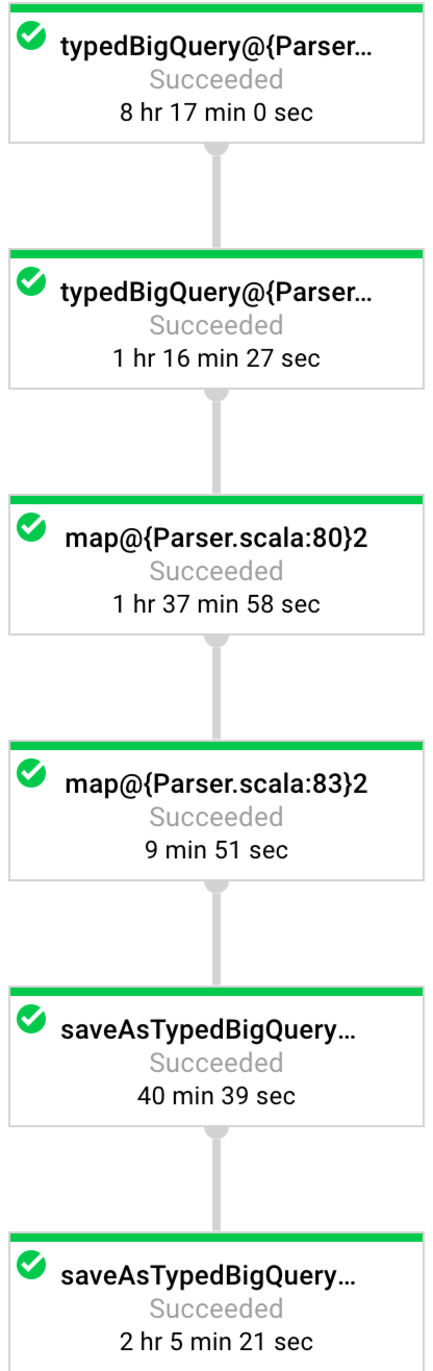
\includegraphics[width=0.5\textwidth,height=0.5\textheight,keepaspectratio]{figures/dataflow.pdf}
    \caption{A parsing job in Cloud Dataflow}
    \label{fig:dataflow}
	\end{figure}

\subsection{Feature Extraction}

After filtering the group of streams from the users that we are interested on and parsing the play context information, the process of extracting and engineering the features can be started. The main goal of this stage is to create the sequential dataset that is going to be used for training the temporal models, while also calculating the binary labels that will indicate whether the users are going to churn or not. Before introducing the resulting features however, understanding how the time range was divided into different windows is utmost importance as to better comprehend how these features are generated.

\subsubsection{Time Windows}

In order to predict whether a user is going to churn in the future or not and generate the churn binary labels, the time sequence is split into two time windows. The \emph{observation window} is the time span where the user behavior is tracked, data which will be used for training the predictor models. It is sequentially followed by a \emph{prediction window} that is exclusively used for generating the churn label. The windows can be better visualized in \autoref{fig:timewindows}. In order to make sure that selected users did not churn a long time before being observed, the last few days of the observation window are used for sampling users who are active, a time span called \emph{activity window}. 

The size of each window is a parameter that shall be experimented on, but a standard length of \emph{56 days} for the observation window, \emph{30 days} for the prediction window and \emph{3 days} for the activity window were chosen by the provider as values that are suitable for the task at hand. This encompass user information gathered from March 5th until May 29th, 2017. Unless otherwise stated, there are going to be the values in use for our experiments.

The user is considered to have churned if he has at least one active stream during the activity window, but no stream during the prediction window, which follows the definition of "churn" from Definition \autoref{def:churn}. An important factor that should be mentioned is that every user will have a single label for the whole sequence, and not a different label per point in time. This can be considered a simplification that reduces the complexity of our predictor models, however it fails to capture users that change between "churned" and "retained" states often: a user that churned may return to the service given more time. Changing the labeling method will be briefly explored in Future Works. \Todo{Add this Future Work}

Our source dataset is sequential by nature. Every interaction is logged and stored in tables representing all streams of users in any given day. However, taking this data as it is is unsuitable to be used for training since commonly temporal models requires that (a) the time step between events to be constant and (b) it possess the same number of samples in every time step. Since there is no control as to when any given user will interact with the application, some data transformations must be performed. 

First, a constantly-sized \emph{time step} was chosen as to split the observations equally across time. To capture the routine of users between every day-night cycles, a time step of 8 hours was deemed to be a suitable value. The features of users are then aggregated over this time range through a mean function. 

Second, the features of users that have no streams in any single time step are set to zero as to keep the number of samples constant through time. This processing will result in a dataset which is quite sparse, since rarely ever a user streams content in all 8 hours time spans over the course of 56 days of observation. An example of this processing can be seen in Figure \ref{fig:zerofill}.

	\begin{figure}[h]
    \centering
    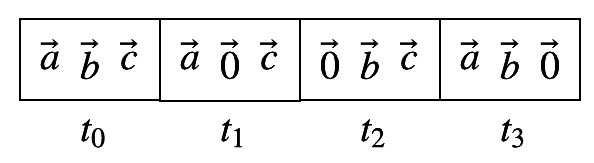
\includegraphics[width=0.7\textwidth, natwidth=580bp, natheight=313bp]{figures/zero_fill.png}
    \caption{Zero-filling 4 time steps for 3 different users}
    \label{fig:zerofill}
	\end{figure}

After applying the previously mentioned transformations, the number of rows of the dataset is severely reduced to \emph{87 million}, mainly due to the 8 hours aggregation procedure.

\Todo{improve the zero-filling figure}

\subsubsection{Features Description}

No dataset would be fully described without a detailed explanation of the features within. This section will be dedicated to exposing the features extracted and engineered from the data sources described in previous sections.

The most basic feature of every stream is its duration in seconds, hereby called \verb|sec_played|, which calculates how long the user playback lasted. Higher values may indicate that users are listening to a song in its entirety, while smaller values may indicate that the user skipped a song or an error occurred, for example. They are not normalized by the duration of the song however, so it may indicate that the song is just shorter in length. The \verb|skip_ratio| indicates the percentage of streams the user skipped comparing to all of his streams, commonly by pressing the "Forward" button on the player. Inter-arrival time (hereby called \verb|iat|) is the time between streams: lower values indicates an user that is constantly using the app, and higher values a user that streams a song every now and then. \verb|total_streams| is simply the count of streams the user had in the current time period, and \verb|sum_sec_played| is an accumulating sum of the feature \verb|sec_played| since the beginning of the observation period. 

After parsing the play context from each stream, we engineer new features by combining them with three of the aforementioned basic ones, which are called \verb|sec_played_<set_type>|, \verb|sum_sec_played_<set_type>| and \verb|total_streams_<set_type>|. Also, the number of unique set types is calculated and aggregated in the feature \verb|unique_top_types|: a previous internal study by the service provider indicates that there is a non-zero relationship between the quantity of features being utilized by the user and its probability of churning, so we engineer and add it to our dataset.

All continuous feature values are aggregated by taking the mean over  each time step period of 8 hours. For the \verb|sec_played| group of features, the standard deviation is also calculated, and it corresponds to the features with the \verb|_std| suffix.

By extracting and combining the features using the methods above, a grand total of 52 features were generated. The correlation matrix between these features can be seen in \autoref{fig:correlation}.

	\begin{figure}[h]
    \centering
    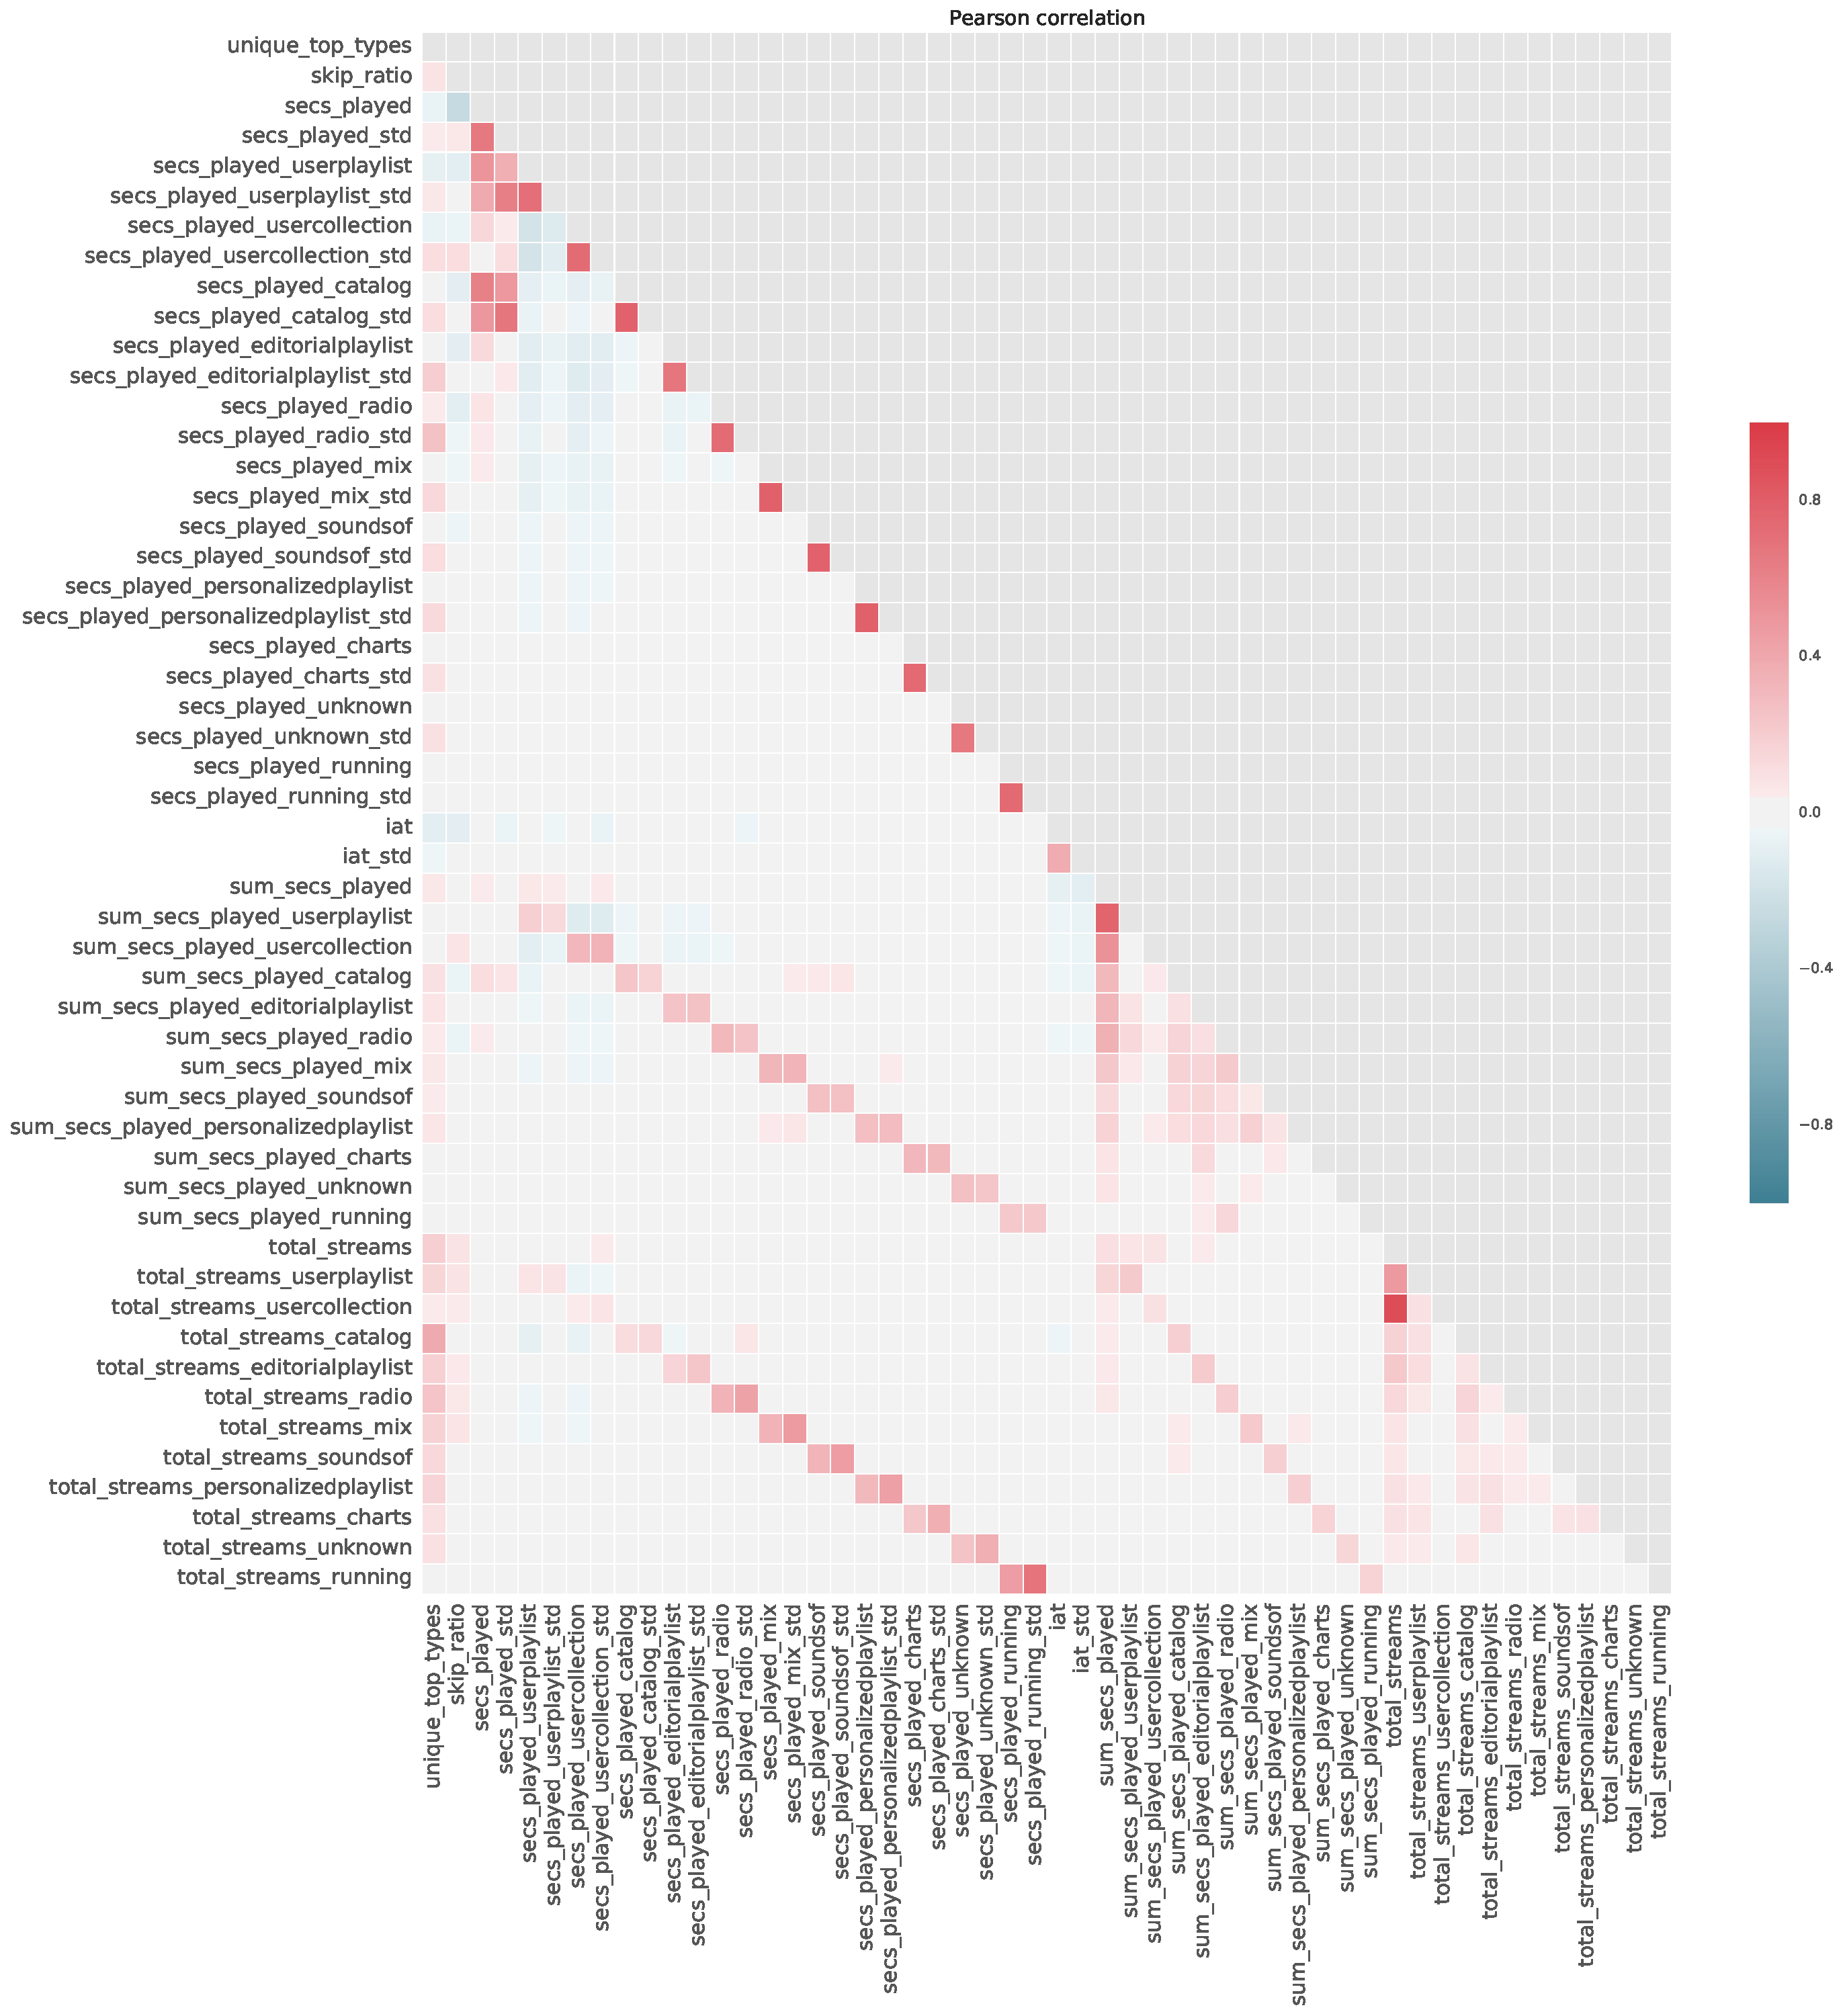
\includegraphics[width=0.9\textwidth,height=0.9\textheight,keepaspectratio]{figures/corr.pdf}
    \caption{Pearson correlation matrix between features}
    \label{fig:correlation}
\end{figure}

\subsection{Data Pre-processing}

The goal of the final stage of the pipeline is to transform the data into a format which is suitable to be used for training and that also improves convergence time of the learning algorithms. This is achieved by two main steps: normalization of the feature values and exporting the data into compressed files.

\subsubsection{Normalization}

While it is possible to use raw features as input to train predictor models, often there is a benefit on normalizing the values using some standard technique. \citep{lecun2012efficient} argues that for the backpropagation algorithm commonly used in neural networks, well-behaved features centered around and with unit variance usually provides a faster convergence time. This is mainly due to the way weights are updated in the network: if the input vector has all features with the same sign, the weights can only be increased or decreased together for a single input, zigzagging the values back and forth which turns to be extremely inefficient. In deep architectures, the output a network layer is used as input to the next layers, and for the same reasons it is also desirable that this input is centered around zero. Inputs with unit variance will keep the layer's output well behaved and thus speed up convergence.

Therefore, the following transformations were applied to the input before the training process:

 \begin{equation}
 \mu_i = \frac{1}{N}\sum_{n=1}^{N}x_n^i
 \end{equation}

\begin{equation}
\sigma_i^2 = \frac{1}{N}\sum_{n=1}^{N}(x_n^i - \mu_i)^2
\end{equation}
 
\begin{equation}
x_n^i = \frac{x_n^i - \mu_i}{\sigma_i^2}
\end{equation}

where $N$ is the total number of samples, $x_n^i$ is a scalar value representing the feature $i$ of the training sample $n$, feature which has mean $\mu_i$ and variance $\sigma^2_i$.

\subsubsection{Aggregating and Exporting}

After normalization, the feature values are in the desired format for training our predictor models, however they are still stored in an unsuitable location to be used as a source since all data is still stored as a table in BigQuery. Streaming the data directly from a cloud provider into the training algorithms, while is possible, depends heavily on the choice of programming language and the available distributed frameworks, and it also susceptible to engineering problems like the network connection between the cloud provider and the host where the models are going be trained on.

For this project, we decided to take a simpler approach and use compressed JSON line-delimited files as a data source for the training procedures. This format can be exported to through Google's web interface and also programatically through BigQuery's API, and be easily loaded using standard libraries in the most popular programming languages. The rows are processed and exported to files in parallel, greatly accelerating the procedure.

We need to take some precautions for the export process to work flawlessly, however. The source table containing all the training data is stored in a long format, that is one row per user per time step. Since the export procedure is performed in parallel, the entries for a single user might end up spread into different files. To avoid having to fix this in the training functions, we apply a simple aggregation by user ID as to group all time steps belonging to a user into a single row. This can easily be accomplished using a query clause and functions in BigQuery.

\section{Data Exploration}

"Get to know your data" is a common jargon in the data science field, and for a good reason: even the smartest learning algorithms may fail to perform well if the data used as source is of questionable quality. Understanding how the data is distributed is of utmost importance, not only to gather insightful information that may be used in our advantage for training our predictor models, but also to validate that our dataset creation algorithm is free of mistakes and is representative of the target audience. This section will be dedicated to visualizing the data created through the pipeline described in the previous sections.

The large amount of rows in the dataset makes it difficult to plot it using standard well-known visualization libraries. Therefore, a sample of 1\% of users was selected for the following plots by applying the same hash plus modulo operator described in \autoref{sec:sampling}, totaling 5.125 unique users and 861.000 rows of data corresponding to the 56 days of observation time.

Due to privacy concerns and the signed non-disclosure agreement between the interested parties in this project, some of the tick labels in the graphs may have been intentionally hidden as to not reveal important business information of Spotify.

\subsection{User Distribution}

A recurring problem in churn prediction is how the non-churning class dominates over the churners for almost all applications, a problem properly examined by \citep{Burez2009}. \autoref{fig:classdist} plots the distribution of classes in our generated dataset. In it we can observe that indeed the churning class is the overwhelming minority of our samples, composing approximately 2.4\% of the data. This heavily imbalanced dataset may pose several challenges when training our models, since learning algorithms may fail to capture the nuances of user churning behaviour with a lack of representative samples.

	\begin{figure}[H]
    \centering
    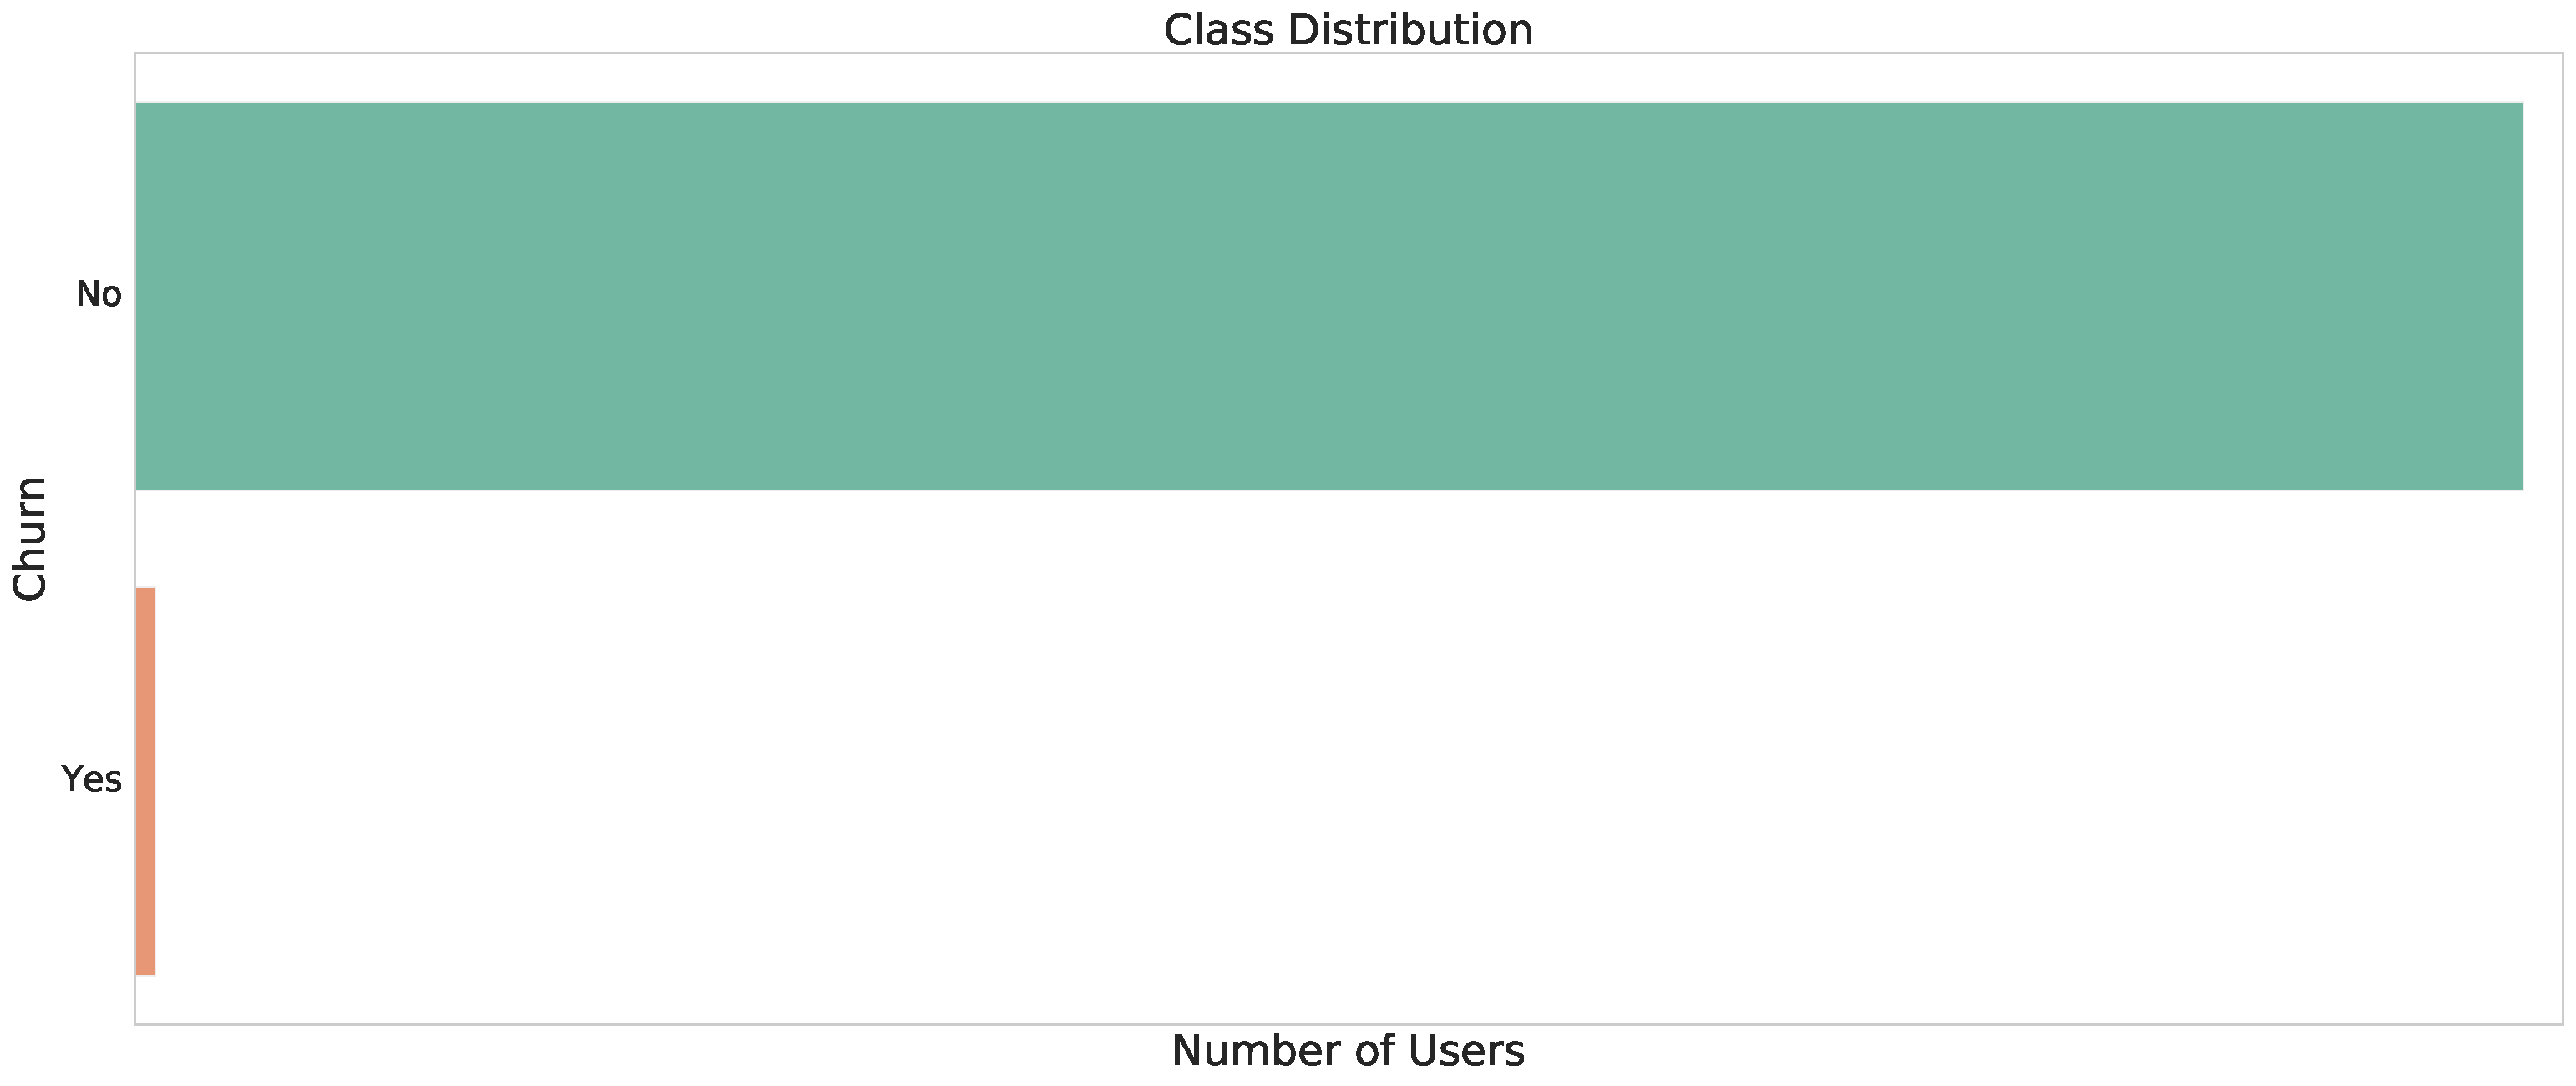
\includegraphics[width=0.9\textwidth,height=0.9\textheight,keepaspectratio]{figures/class_dist.pdf}
    \caption{Count of users distributed in the churn and non-churn classes}
    \label{fig:classdist}
	\end{figure}

Spotify has several different product types in its catalog. They can however be aggregated into two main categories with minimum loss of information, and that would be the ad-supported \emph{free} version and all the different subscription-based paid versions called as \emph{direct} by the provider. Visualizing the data by plotting against the different product types can be seen in \autoref{fig:proddist} and it reveals something interesting, albeit predictable: the majority of the churning users belong to the free tier, which is understandable due in parts to how easy it is to abandon the service without a formal contract attached, and also by the negative ad-filled experience that users are exposed to. \Todo{add a ref here from pilot study}

	\begin{figure}[H]
    \centering
    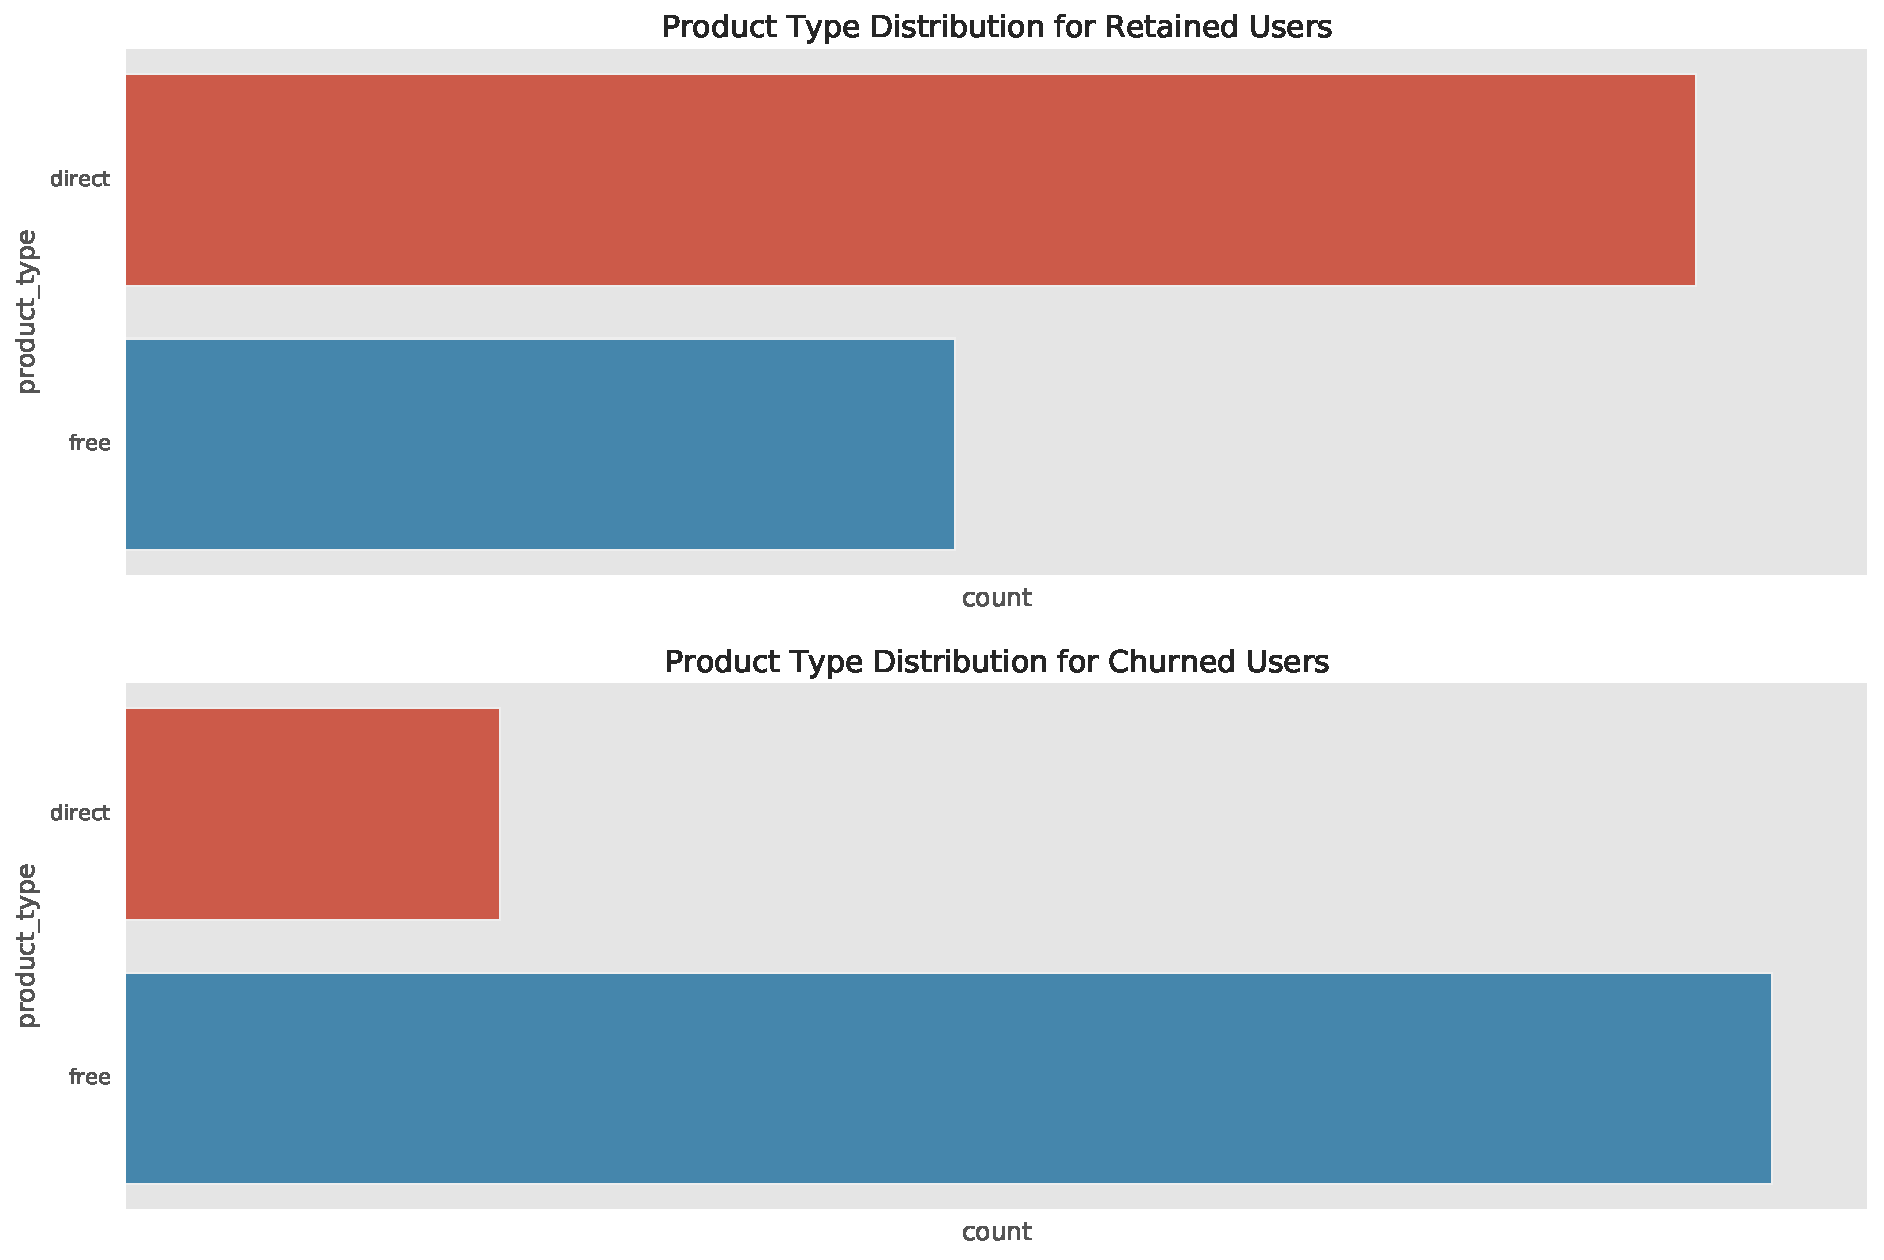
\includegraphics[width=0.99\linewidth,height=0.9\textheight,keepaspectratio]{figures/dist_product_type.pdf}
    \caption{Users distribution per product type and churn label}
    \label{fig:proddist}
	\end{figure}

In this project, three different markets were the focus of the study, so it would sensible to visualize how the distribution of the data differs for each single country. In \autoref{fig:countrydist} we can distinguish how the majority of sampled account belongs to users from US. Brazil and Mexico have a similar distribution for the retained class, however there is significantly more churning users in Brazil. \Todo{Ask Sahar why is that}.

	\begin{figure}[H]
    \centering
    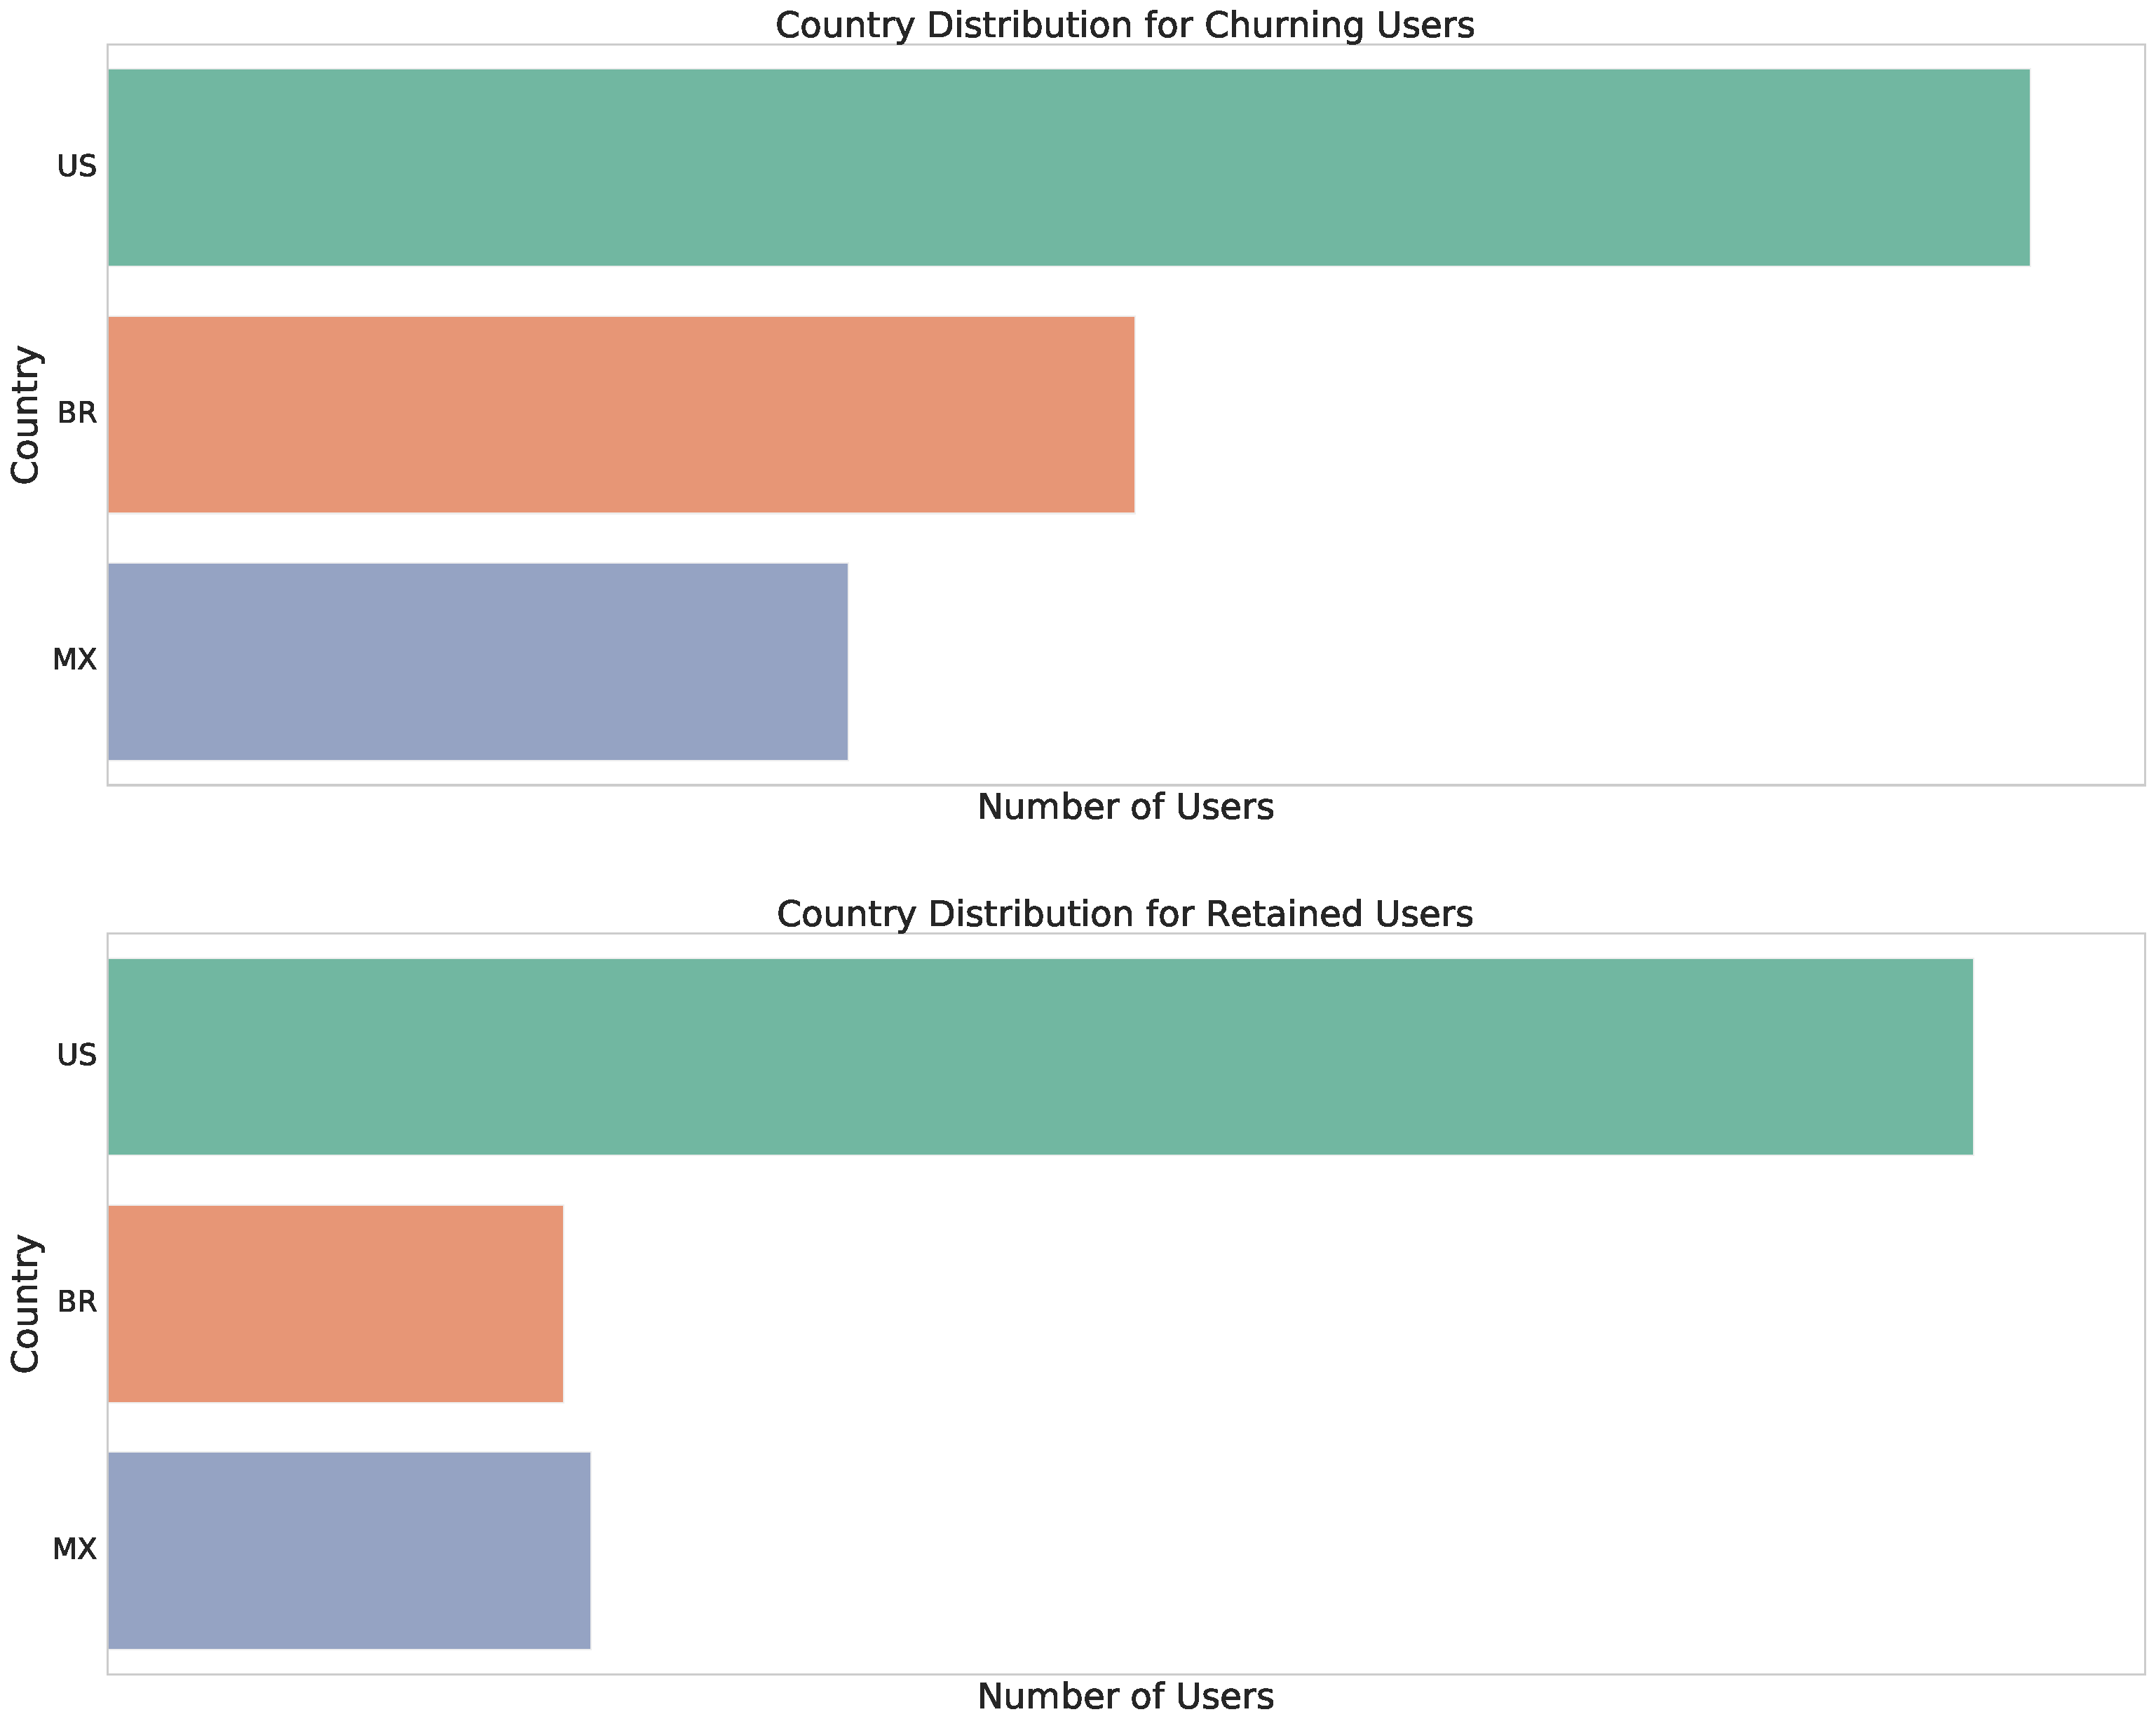
\includegraphics[width=0.9\textwidth,height=0.9\textheight,keepaspectratio]{figures/dist_reporting_country.pdf}
    \caption{Users distribution per country and churn label}
    \label{fig:countrydist}
	\end{figure}

Users in Spotify possess different behaviors whether they registered for a long time or if they just created their accounts. Internal studies showed that long-term users reveal a more stable behavior on application usage when comparing to recent arrivals. Also, activating new users into the platform is a challenge in itself, since the service is unknown they are more susceptible to abandoning if they dislike the features they were exposed to. \autoref{fig:dayssinceregdist} plots the number of days since registration between the churning and retained classes, it can be visualized how churning users are concentrated on the range of new users, while the retaining class is more uniformly distributed along the x-axis.

	\begin{figure}[h]
    \centering
    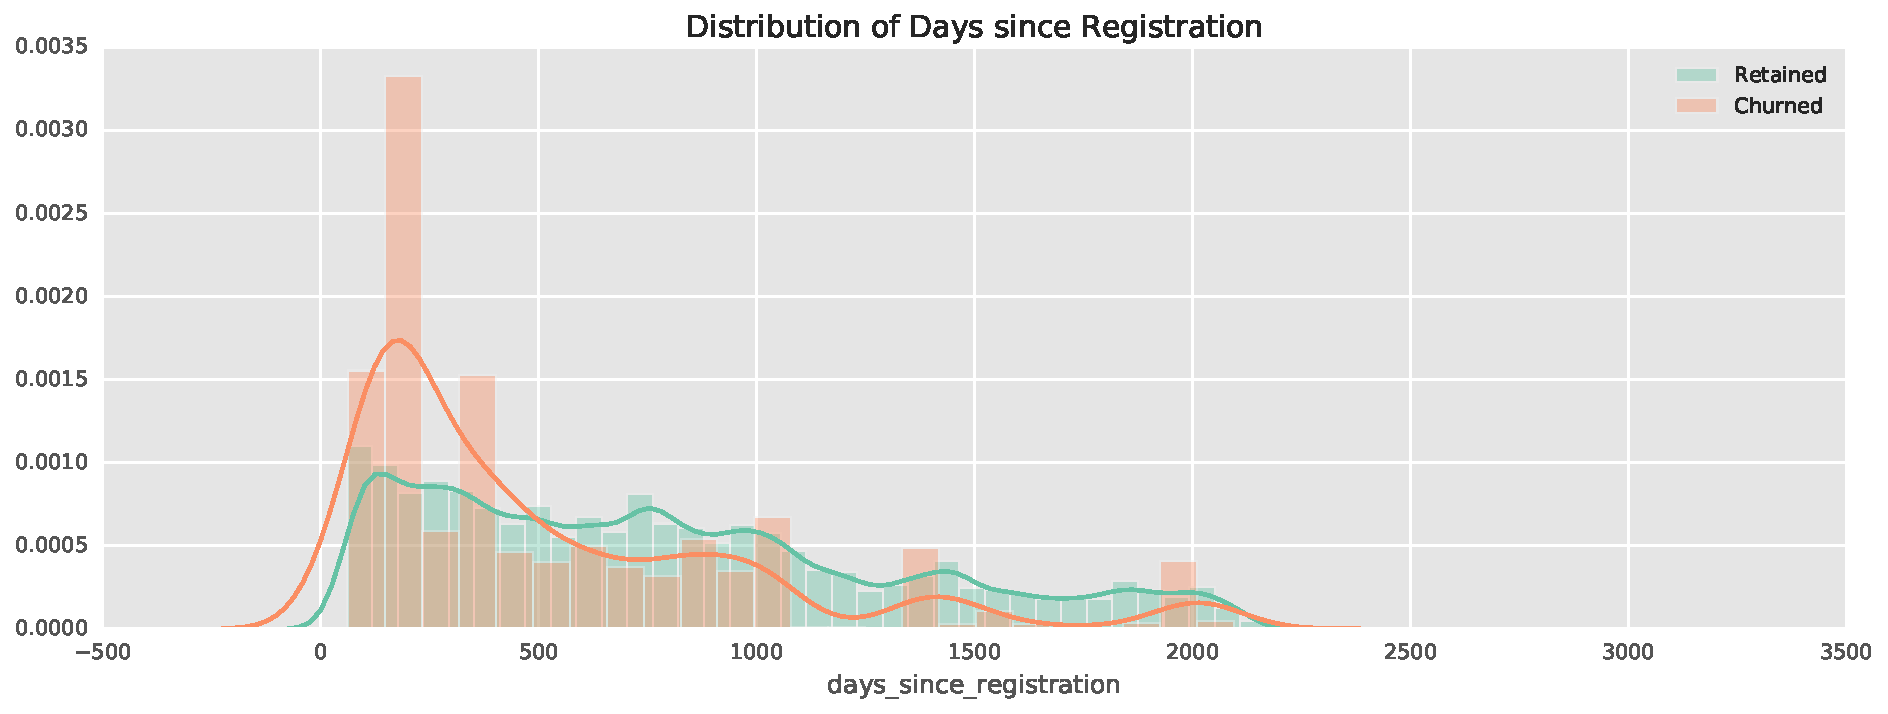
\includegraphics[width=0.9\textwidth,height=0.9\textheight,keepaspectratio]{figures/dist_dayssincereg.pdf}
    \caption{Users distribution over days since registration and churn label}
    \label{fig:dayssinceregdist}
	\end{figure}

\subsection{User Behavior Through Time}

Humans are creatures of habits. Our daily routines follow distinguishable patterns mainly influenced by day-night cycles that are far from being random. To better visualize these patterns, \autoref{fig:featstime} plots the feature values for churning and retaining users over the course of the observation window sized at 56 days. 

The first pattern that can be noticed is that users that are labeled as churning have lower values for features when to those who are retained in the service. This difference can greatly be perceived in the \verb|sec_played| (the average number of seconds in all streams in the time step), \verb|total_streams| (the count of streams in each time step) and \verb|sum_sec_played| (the accumulating sum of seconds played in streams. These are all features that indicate usage: users that interact with the application more often and for more time are more likely to be retained.

The second trait that can be observed is that the gap between the classes for the \verb|skip_ratio| feature is smaller than others. A previous study from the service provider suggests that users who churn have higher skip ratio values, however this is counter-balanced by the fact that free users have an artificial limit for skips in the application, currently limited at 5 per hour \Todo{Check with Sahar}. This may be the root cause for this behavior, since free accounts are the majority of the churning class, as could be seen in \autoref{fig:proddist}.
	
	\begin{figure}[h]
    \centering
    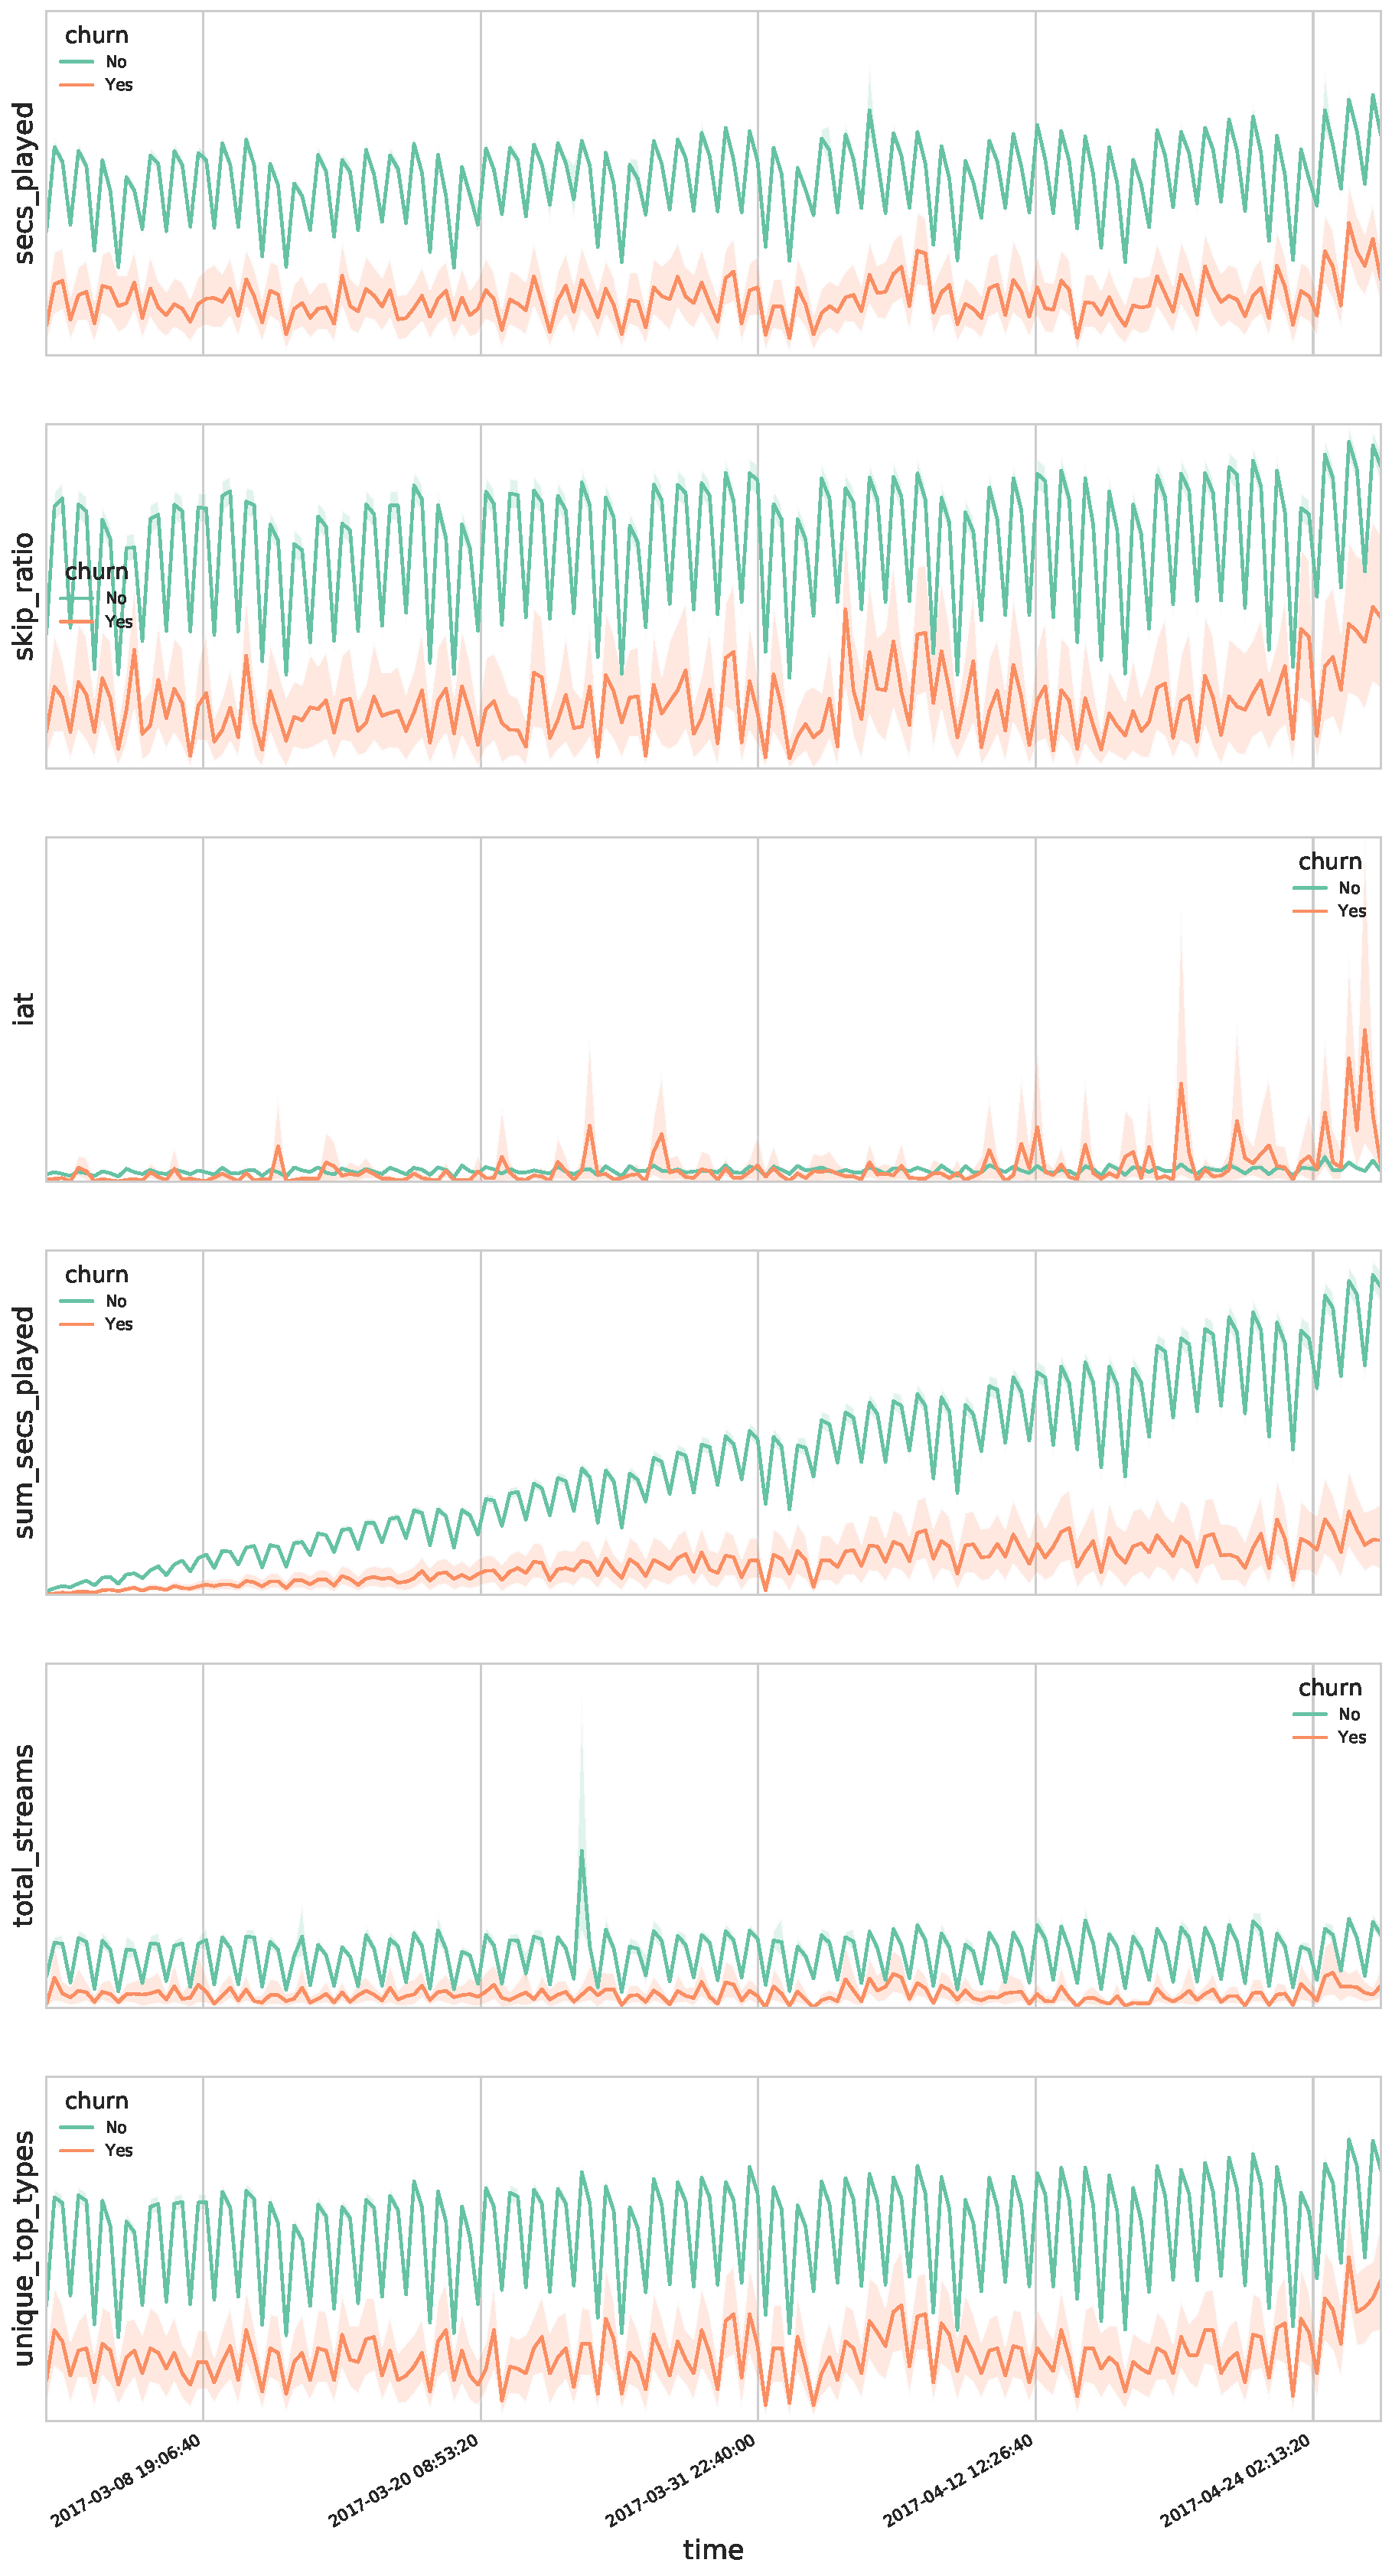
\includegraphics[width=0.9\textwidth,height=0.9\textheight,keepaspectratio]{figures/feats_time.pdf}
    \caption{Mean values of features throughout the observation window}
    \label{fig:featstime}
	\end{figure}

\subsection{Feature Correlation to Churn}

One question that can be answered is how does any of the generated features correlates to the churn label. Do they exhibit a positive or negative association? Even though it is known that correlation does not necessarily implies a causal relationship, it may still be interesting to observe what is the overall tendency of the features when they are associated with churn. To accomplish this, a \emph{point biserial correlation coefficient} is the correct tool to use when one of the variable is continuous and the other dichotomous, and its plot can be seen in \autoref{fig:corr_pbs}.

Some interesting relationships can be observed. First, the plot shows that \verb|iat| features (inter-arrival time between streams) are the ones with the strongest association to the positive churning label, which is understandable: users that do not come back to the application as often are not making use of the service at its fullest and are more likely to abandon it. Second, the \verb|sum_sec_played| group of features are in its majority negatively correlated with churn, which strengthens our hypothesis that customers who use the service more often are less likely to abandon it. 

Another interesting fact is that not all set types have the same association with our label: while \verb|user_playlist| and \verb|personalized_playlist| have the strongest negative association with churn of all available set types, while users that have longer streams of \verb|editorial_playlist| are more correlated with a positive value churn. Again, this does not imply that there is a causal relationship between the two, but may be a good tip towards investigating how this feature is delivered to the user.

Lastly, a rather surprising result is that the number of unique set types have a positive association with churn. Our hypothesis is that users who are new in the platform posses a more explorative behavior by trying several different features when compared to users who are in the platform for a long time. As could be seen in \autoref{fig:dayssinceregdist}, churning users are commonly younger in the service when compared to retained ones. 

	\begin{figure}[H]
    \centering
    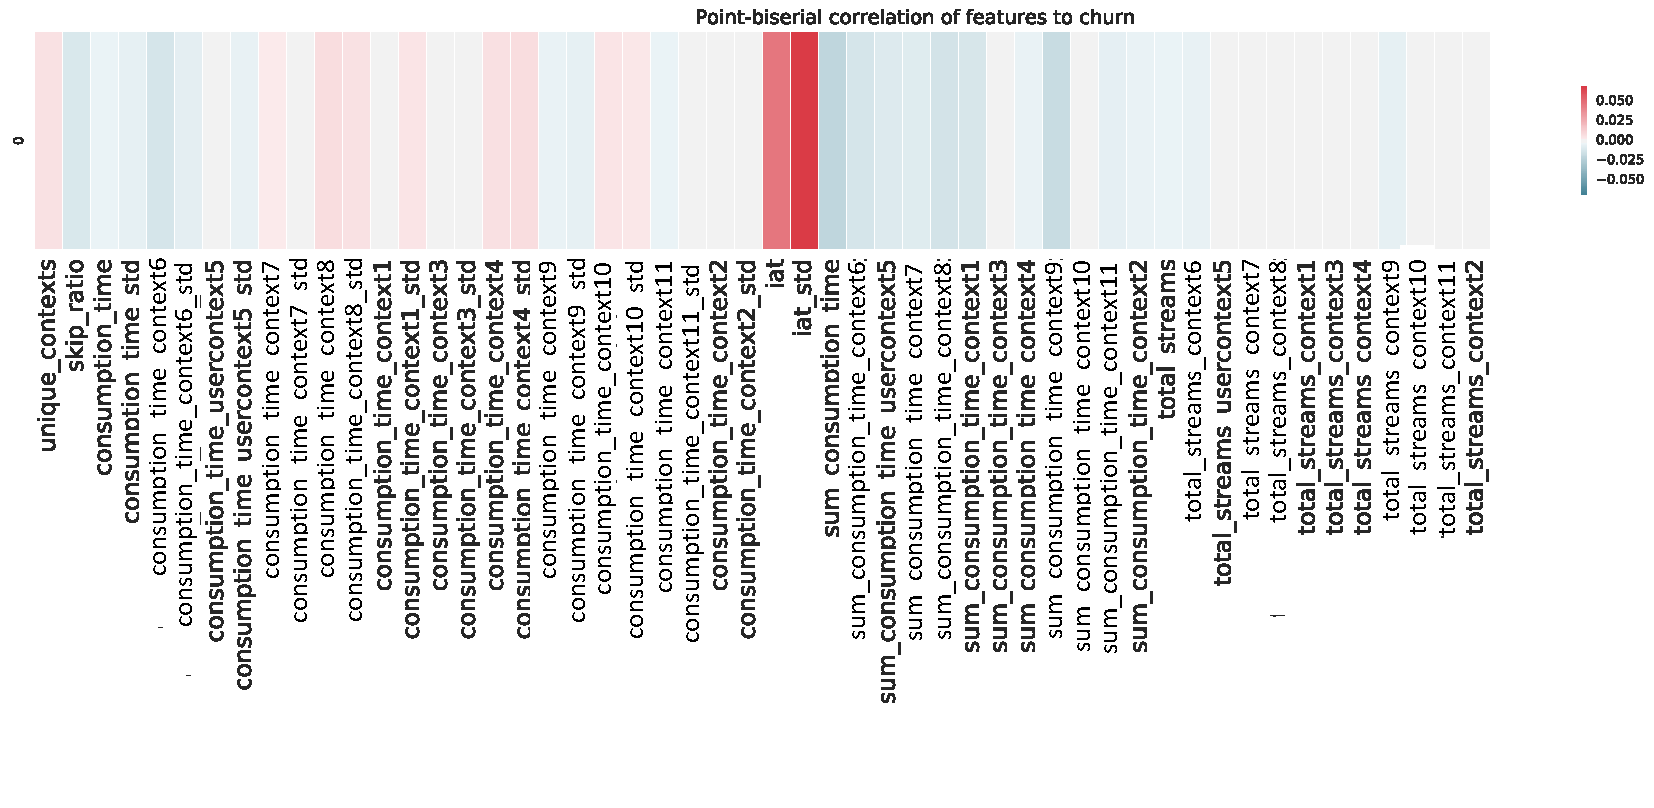
\includegraphics[width=0.9\textwidth,keepaspectratio]{figures/corr_pbs.pdf}
    \caption{Point-biserial correlation between features and the churn label}
    \label{fig:corr_pbs}
	\end{figure}

\subsection{Dimensionality Reduction}

Although the features generated through our data pipeline encompasses different aspects of the users behavior in the platform, it may pose a challenge regarding the high dimensionality of our dataset: machine learning models may have trouble extracting the latent information from feature values if data is not sufficient. Since our dataset is heavily imbalanced, the number of available samples for the churning class may be insufficient, and using a more compact representation of the data may prove fruitful when the goal is to maximize the score of our predictor models.

Principal Component Analysis (PCA) is popular technique that strives to find a lower dimension representation by keeping most of the variability of the data, or as described by Hotelling \citep{hotelling1933analysis}, it is, for a given set of data vectors, the $d$ orthonormal axes onto which the variance retained under projection is maximal.

In \autoref{fig:pca_data} we can visualize the data distribution when its dimensionality is reduced to its two principal components through PCA for both retained and churned classes. It can be seen that even though the overall shape of the distributions are clearly different, their center points are not that close to each other, which may result in difficulties when trying to find a hyperplane that bests separates both retained and churning classes.

	\begin{figure}[h]
    \centering
    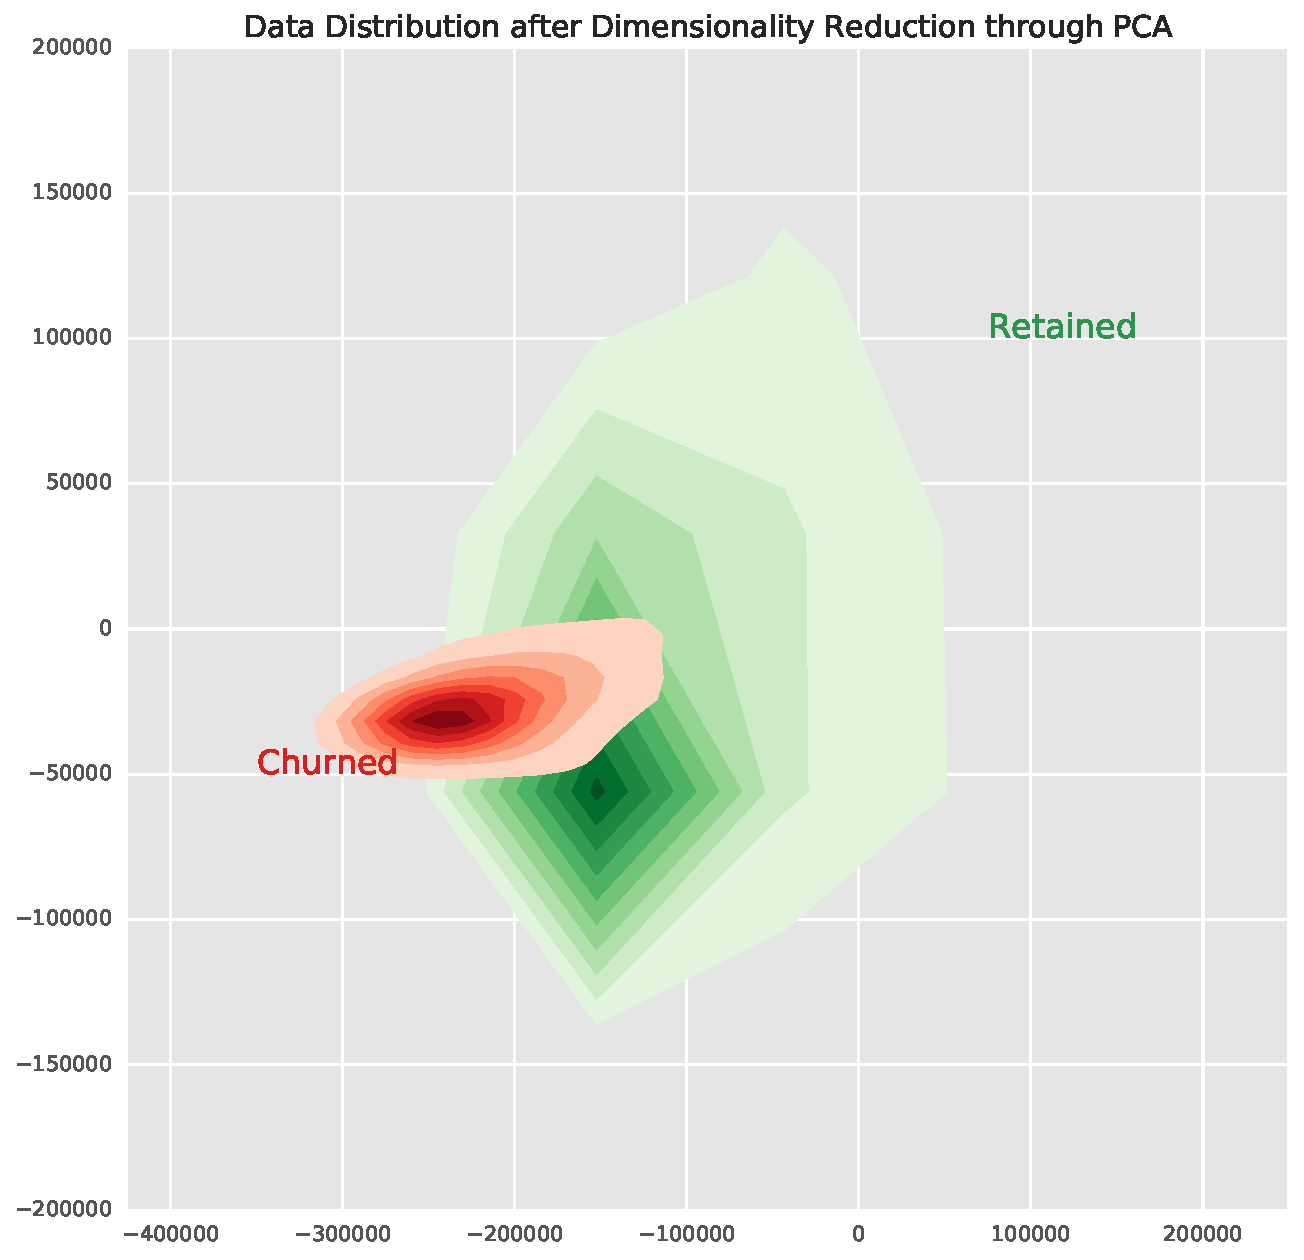
\includegraphics[width=0.9\textwidth,keepaspectratio]{figures/pca_data.pdf}
    \caption{Data distribution after reducing to 2 principal components through PCA}
    \label{fig:pca_data}
	\end{figure}

\section{Software and Libraries}

Manipulating large quantities of data is a task that cannot be performed easily using standard libraries of a programming language. The pipeline creation was only made possible in the scope of this project by making use of frameworks for massive data manipulation available at Spotify.

The sampling, extraction and pre-processing steps of the data pipeline were performed using Big Query\citep{sato2012inside}, a fully-managed and cloud-based interactive query service for massive datasets created by Google. The parsing step that extracted the type of the stream from its play context was performed in Scio\citep{scio}, a Scala API for Apache Beam and Google Cloud Dataflow.

\chapter{Methodology}

Creating experiments that are reliable, reproducible and as unbiased as realistically possible is a challenge for any researcher interested in obtaining results that can safely be reasoned on. It is made harder by the complexity of our own source dataset: human behavior is far from being a process easily predictable due to the sheer amount of latent variables that may influence the outcome of the experimentation process.

This chapter is dedicated to present to the reader a detailed picture how the experiments were performed, the choices of classifiers, the way they were optimized to the best set of parameters, and how the final score for each model was obtained.

\section{Handling the Class Imbalance Problem}

For any relatively successful company the non-churning class heavily outweigh the amount of churners in the dataset. Depending on the estimator, this property can have a negative impact in performance where the models only can only learn how to distinguish the majority class and failing to detect the class of interest. However empirical observations have shown that a better performance can be achieved if the class ratio difference is reduced \citep{Burez2009} \citep{ling1998data}. 

There are three commonly used sampling techniques for dealing with heavily skewed datasets: 

\begin{itemize}
\item Undersampling by removing samples from the majority class using a pre-defined selection technique
\item Oversampling by creating artificial samples that closely mimics the true data present in the minority class
\item A combination of over and undersampling, commonly oversampling the minority class first and reducing the data in the majority class second.
\end{itemize}

Unless otherwise stated, the experiments in this project will be \emph{randomly undersampled} to a class ratio of 1-to-1. This technique, while easy to implement, throws away several samples from the majority class that could be used for learning. Testing different ratios for the class distribution is however one of the experiments that will be performed in this project. Different methods for under and oversampling will be further discussed in Future Works \Todo{add over undersampling talk in future works}.

\section{Cross-Validation}

It is a common  practice in supervised machine learning experiments to split the data sets into \emph{train} and \emph{test sets} as to obtain an unbiased estimate of the performance of the trained models on unseen data: evaluating a model on the data it was trained on can return an overly optimistic score that does not generalize well for data that is not included in the training, a phenomenon called \emph{overfitting}. Therefore, every score in this project is reported using data that was not present in the training stage.

Almost all machine learning predictor models have arguments that needs to be chosen even before the training process starts, values that are commonly called \emph{hyperparameters}. To fine tune these parameters, we need a method to evaluate how good a set of values are against all other (or a reasonably sized subset of) available options, and for that purpose we need a set of unseen data for the same reasons mentioned before. If the test set were used for such an evaluation, it could not be considered as unseen data anymore since it was used for the purpose of choosing the best model, thus our bias may have "leaked" to the prediction score. Therefore another set is needed to tune the hyperparameters, which is commonly called the \emph{validation set} in the machine learning domain.

Dividing the dataset into three splits however drastically reduces the number of samples that ares available for model learning. Another concern is that if the sets are unique, the overall performance metric will depend in a seemingly random split of validation and test sets. To mitigate this problem, a technique called \emph{cross-validation} can be applied\citep{stone1974cross}. In its most basic approach, instead of having a single validation set, the training set is instead divided into $k$ folds, and at each hyperparameter tuning round the model is trained on $k-1$ folds and validated on the fold that was left out. For each set of parameters, $k$ models are generated, and the final metric can then be an aggregation function over all estimators performance, like the mean. After selecting the best set of parameters, another training session can be made with the union of the data available in all folds, thus acquiring a tuned version of the model.

The above technique helps to strengthen our performance metric against biases when selecting the best set of hyperparameters to train our model with. However we still have an unique test set where we evaluate our model to obtain a final score. When comparing different types of estimators, it may happen that one estimator may better learn from the samples that are on the training set while the other can better learn from the patterns contained on the samples of the test set, a split that was purely made by chance. This may lead to a form of selection bias resulting in overly-optmistic scores \citep{cawley2010over}. The same procedure used for hyperparameter tuning can be applied for splitting the train and test sets, a technique called \emph{nested cross-validation}. In it, the full dataset is split into $k$ outer folds of training and test sets, and each training set is further split into $l$ inner folds for hyperameter tuning.  A diagram of this procedure can be seen in Figure \ref{fig:crossval}.

	\begin{figure}[h]
    \centering
    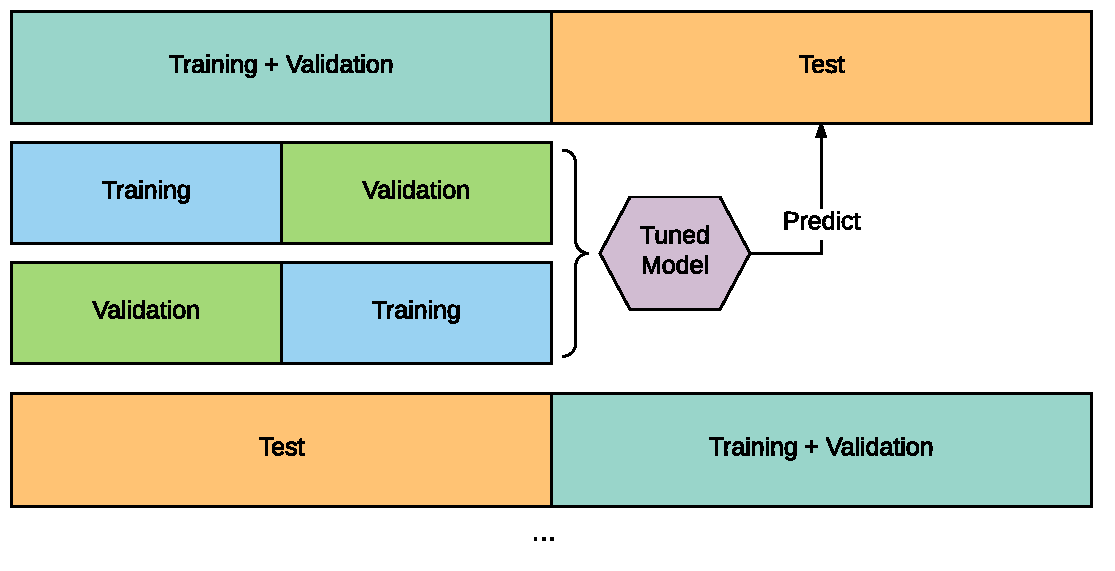
\includegraphics[width=0.8\textwidth,keepaspectratio]{figures/crossval.pdf}
    \caption{2x2 nested cross validation}
    \label{fig:crossval}
	\end{figure}

Even though this technique increases the confidence of our metric scores, there is a price to pay in terms of performance: training all these models may take a considerable amount of time. Spotify however has no lack of computational resources available, so this project makes use of this method. Inspired by \citep{Burez2009}, all our models were trained using \emph{2$\times$2 cross-validation}, with 2 outer folds for the train/test split and 2 inner folds for train/validation splits.

\section{Hyperparameter Search}

Lastly, a proper method needs to chosen to perform search over the domain of parameter values. A common practice in machine learning model training is to perform a parameter sweep by exhaustively searching a subset of values manually chosen by the experimenter. This method is called \emph{grid search}, and due to its simplicity and reproducibility is one of the most used techniques, be it for classical machine learning algorithms like Support Vector Machines as to deep feed-forward neural networks \citep{larochelle2007empirical}.

However, performing a grid search over every combination of values can quickly turn it into a method which is too computationally expensive to perform for any real-world applications. Deep architectures like LSTMs are known to be costly to train, and combining it a full parameter sweep is prohibitive if the dataset in question is of a respectable size. Bengio and Bergstra\citep{bergstra2012random} have demonstrated that, for neural networks, performing a \emph{random search} over the same parameters domain can result in a model which is as good or better than the one validated through grid search by using a fraction of the computation time. 

In a random search, parameter values are randomly sampled from a specified distribution instead of being chosen directly from a grid. For a set number of rounds, samples are gathered for every parameter and used for model validation. This allows us to set a processing budget which is independent of the number of parameters available and the number of possible values for each. Therefore, adding parameters that have no impact in performance will not decrease the efficiency of the cross-validation process for no gain. 

The experiments performed in this project make use of both methods: for the classical Logistic Regression and Random Forests, a grid search over a pre-selected set of values was the chosen method, since their training time is commonly faster when compared to regularly sized deep neural network. Random search is the technique used for validating parameters of our LSTM models, since it is too expensive to compute with a parameter sweep due to its long training time. The set of parameters used for the experiments follows:

\begin{itemize}
\item Logistic Regression
\begin{itemize}
\item C (inverse of regularization strength): 0.01, 0.1, 1, 10, 100
\item Regularization method: L1-norm, L2-norm
\end{itemize}
\item Random Forest
\begin{itemize}
\item Number of estimators: 10, 100, 500, 1000
\end{itemize}
\item LSTM
\begin{itemize}
\item Number of layers: 1 to 3
\item Units per layer: 64 to 256
\item Optimizer: RMSprop, Adagrad
\end{itemize}
\end{itemize}

\section{Model Training}

Even though all models were trained with the same source dataset, temporal and time-invariant models requires a different representation of the data, a topic which was explored in \autoref{sec:timewindows}. Logistic regression and random forest models were both trained with the SPTD version of the dataset using the mean as the aggregation function $f()$, while the LSTM models were trained with the full unrolled MPTD data.

When analyzing the data contained in the MPTD dataset, it can easily be noticed that is severely sparse. This is due to the representation chosen for the absent user in a specific time step: users that did not stream any song during an 8 hours interval will have its features all set to zero. We can leverage this property through a data structure that better utilizes memory resources by storing only the non-zero entries instead, which is accomplished by representing the data with a \emph{compressed sparse row} structure \citep{bulucc2009parallel}. This allows us to store the data in memory in a single machine without resorting to distributed algorithms which would make the implementation more difficult.

To increase the reproducibility of our experimentation process, the same seed value was used for all random factors contained in the experiments. That includes the dataset fold splitting, random search, weights initialization in LSTMs and the undersampling. The seed value chosen was 42, which is the answer to the ultimate question of life, universe and everything \citep{adams1995hitchhikers}.

\subsection{The LSTM Recurrent Network}

This section describes some details about the LSTM models used in the experiments of this project.

Since the number of layers is a parameter that is being tuned during the cross-validation phase, the exact architecture of the LSTM varies depending on the training and validation data. It is beneficial however to visualize the overall structure of one choice of model parameters as to better understand how the layers are organized, which can be seen in \autoref{fig:lstm_arch}.

	\begin{figure}[h]
    \centering
    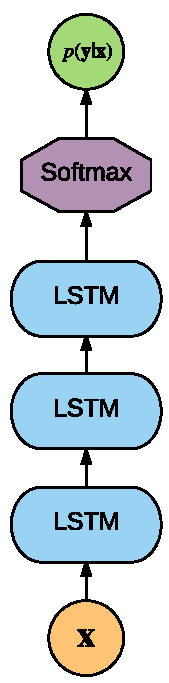
\includegraphics[height=0.7\textwidth,keepaspectratio]{figures/lstm_arch.pdf}
    \caption{Model architecture with 3 stacked LSTM layers}
    \label{fig:lstm_arch}
	\end{figure}

In this example, three LSTM layers were stacked on after the other, each one with a different number of units per layer chosen through random search. A softmax layer transforms the output of the last LSTM layer and transform it into a probability distribution over the two retained and churned classes.

Every model was trained for 100 epochs using a batch size of 512, a number chosen for performance reasons. The optimizers were initialized with a learning rate of 0.001. For Adagrad, the value for the fuzz factor $\epsilon=1\times10^{-8}$ applies. RMSProp also has the same $\epsilon$, adding $\gamma=0.9$ which regulates how much of the previous average of gradients shall be used to calculate the current gradients .

The weight matrices for the linear transformations of the input were initialized with Xavier initialization method, while the ones corresponding to the linear transformation of the recurrent state were initialized with a random orthogonal matrix. Bias vectors were initialized to zeros since the asymmetry breaking is already performed by the chosen weight initialization algorithm.

The loss function is binary cross entropy. All parameters were regularized with $L_2$ weight decay method, using a regularizing factor of $0.01$.

\subsection{Training Procedure}

We summarize the training process in Algorithm \autoref{alg:train}. This procedure is applied for every different classifier that we are currently experimenting on, and results in a probability score assigned for every sample in the dataset.

The first step of the procedure finds all the parameter values that the models are going be validated on, which can be either a full parameter sweep for Random Forests and Logistic Regression or through randomly sampling from parameters distributions for an LSTM. This will define the size of the innermost loop of the algorithm. 

The outermost loop iterates two times by splitting the input data into two halves and selecting one fold to be the training set and the other the test set at each turn. After this split, the training data (and \emph{not} the test set) is randomly undersampled to the specified ratio, commonly 1-to-1 unless this is a parameter that is actually being experimented on. Since our dataset is heavily imbalanced, this reduces the number of samples significantly.

The second for-loop iterates also two times and splits the undersampled training data further into two sets: training and validation. Finally, a model is trained for each choice of hyperparameter for that specific classifier, resulting in a score for that parameter for that fold. The best hyperparameter is then selected to be the one with the best average score over the 2 folds, which is then used to train a new model with the training the whole training data obtained from the first topmost split.

After the training of the tuned model is finished, it is used to calculate the probability scores of each sample in the test set. These scores are stored in memory, and the process is repeated by switching the roles of the test and training sets. When the whole procedure is finished, every sample from the dataset will have a probability score assigned to it calculated when that sample was part of the test set.

 \begin{algorithm}
\caption{Training and evaluating procedure using nested cross-validation}
\label{alg:train}
\begin{algorithmic}
	\REQUIRE $indata:$ input data 	
	\ENSURE $preds:$ predictions for every input sample when they were part of the test set 
	\STATE $params \Leftarrow gridOrRandSearch()$ 
	\FOR{$trval, te$ in $2fold(indata)$}
		\STATE $trval \Leftarrow undersample(trval)$ 		
		\FOR{$tr, val$ in $2fold(trval)$} 
			\FOR{$p$ in $params$} 
				\STATE $model \Leftarrow train(tr, p)$
				\STATE $scores[p] \Leftarrow evaluate(model, val)$	
			\ENDFOR
		\ENDFOR
		\STATE $p \Leftarrow argmax(avg(scores))$
		\STATE $model \Leftarrow train(trval, p)$
		\STATE $preds \Leftarrow predict(model, te)$
	\ENDFOR	
	\RETURN $preds$
	    
\end{algorithmic}
\end{algorithm} 

\section{Evaluation Metrics}

\subsection{Confusion Matrix}

A \emph{confusion matrix} (also called contingency table) is a table layout representing the performance of a classifier's output, judging by its predictions against the actual true values. In a binary classification problem, the confusion matrix is a 2 x 2 table where commonly the rows represent the true labels while the columns the predicted classes. Each cell contains a count of how many samples were classified on that category, and the values in the diagonal represent the correctly classified samples (if the features are ordered). Figure \ref{fig:confusion_example} depicts a sample confusion matrix for a binary classifier.

\begin{figure}[h]
    \centering
    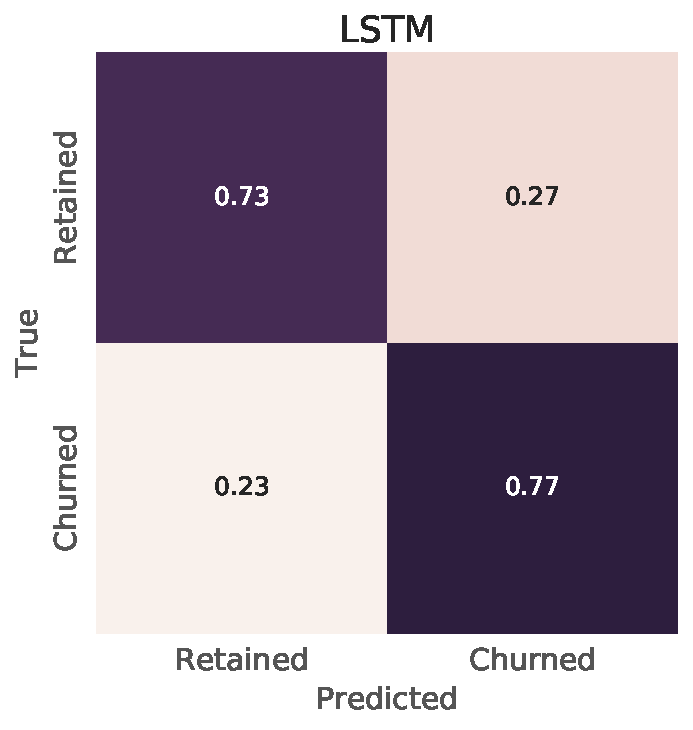
\includegraphics[width=0.5\textwidth,keepaspectratio]{figures/confusion_example.pdf}
    \caption{An example of a normalized confusion matrix}
    \label{fig:confusion_example}
\end{figure}

The confusion matrix is an excellent visualization tool to estimate the performance of a model. The values that should be maximized, the \emph{true positives} (TP) and \emph{true negatives} (TN), represent the samples that were correctly labeled as possessing the feature of interest or not, respectively. On the other hand, the \emph{false positives} (FP) and \emph{false negatives} (FN) are the misclassified samples where the algorithm predicted that the feature was present while in truth it was not and vice-versa. In this work, the positive class will always represent a churning user, and it follows that the negative class represents the non-churners.

\subsection{Classification Accuracy}

Several different metrics can be derived from the confusion matrix table. The \emph{classification accuracy} (CA) of a model is a common metric that corresponds to the fraction of the correctly classified samples on the test set, and can be calculated as follows:

\begin{equation}
CA = \frac{TP + TN}{TP + TN + FP + FN} 
\end{equation}

While trivial to understand, this metric may lead to erroneous conclusions when class imbalance is present in the test set, which is a common occurrence on the churn prediction domain. For example, if 9 out of 10 users of a dataset are non-churners, any classifier that simply outputs a negative class for all samples will result in an accuracy of 90\%, however its ability of detecting churners is non-existent. For a service provider, detecting churn cases is always more important than detecting the loyal users, and this metric by itself cannot represent this goal \citep{Burez2009} \citep{Hassouna2015}.

\subsection{Precision, Recall and Other Metrics}

To address the class imbalance problem of the classification accuracy, others metrics are also commonly used. The \emph{positive predictive value} (PPV, also known as precision) is the proportion of the samples labeled as positive which are true positives, and describes the performance of the algorithm. The \emph{true positive rate} (TPR, also called sensitivity and recall) of a model corresponds to the number of correctly predicted positive samples divided by all positive samples. \emph{True negative rate} (TNR, also called specificity and fall-out) is the number of correctly predicted negatives divided by all true negatives. The \emph{false positive rate} (FPR, also called false alarm ratio) is the probability of receiving a false positive as output of an experiment, and is calculated by dividing the number of false positives by the total number of positive samples. The \emph{F1 score} (F1, also called F-score or F-measure) builds upon precision and recall by returning an harmonic mean between these two metrics.

\begin{equation}
PPV = \frac{TP}{TP + FP}
\end{equation}

\begin{equation}
TPR = \frac{TP}{TP + FN}
\end{equation}

\begin{equation}
TNR = \frac{TN}{TN + FP}
\end{equation}

\begin{equation}
FPR = \frac{FP}{TN + FP} = 1 - TNR
\end{equation}

\begin{equation}
F1 = 2 \times \frac{PPV \times TPR}{PPV + TPR}
\end{equation}

Depending on the distribution of classes of the dataset, it is often difficult (although desirable) to maximize both precision and recall metrics at the same time. A compromise must be reached that achieves the best trade-off between the two, which is commonly a business decision. For a music streaming service like Spotify, maximizing sensitivity is preferred due to the costs associated with a churning user, however a reasonable specificity is also a metric that should be strived for. \Todo{Check with Sahar}

\subsection{Receiver Operating Characteristic}

The \emph{receiver operating characteristic} (ROC) is a visualization tool that plots the relationship between the true positive rate (commonly the y-axis) and the false positive rate (the x-axis) of a binary classifier system. The curve is drawn by selecting different parameters of a model or levels of threshold for the decision boundary between the positive and negative classes. For example, when the output of a classifier is a probability value (like in logistic regression), different thresholds can be chosen to decide whether a user is a churner or not, depending if the goal is to minimize FPR or maximize TPR. An example of a ROC curve can be seen in Figure \ref{fig:roc_example}.

\begin{figure}[h]
    \centering
    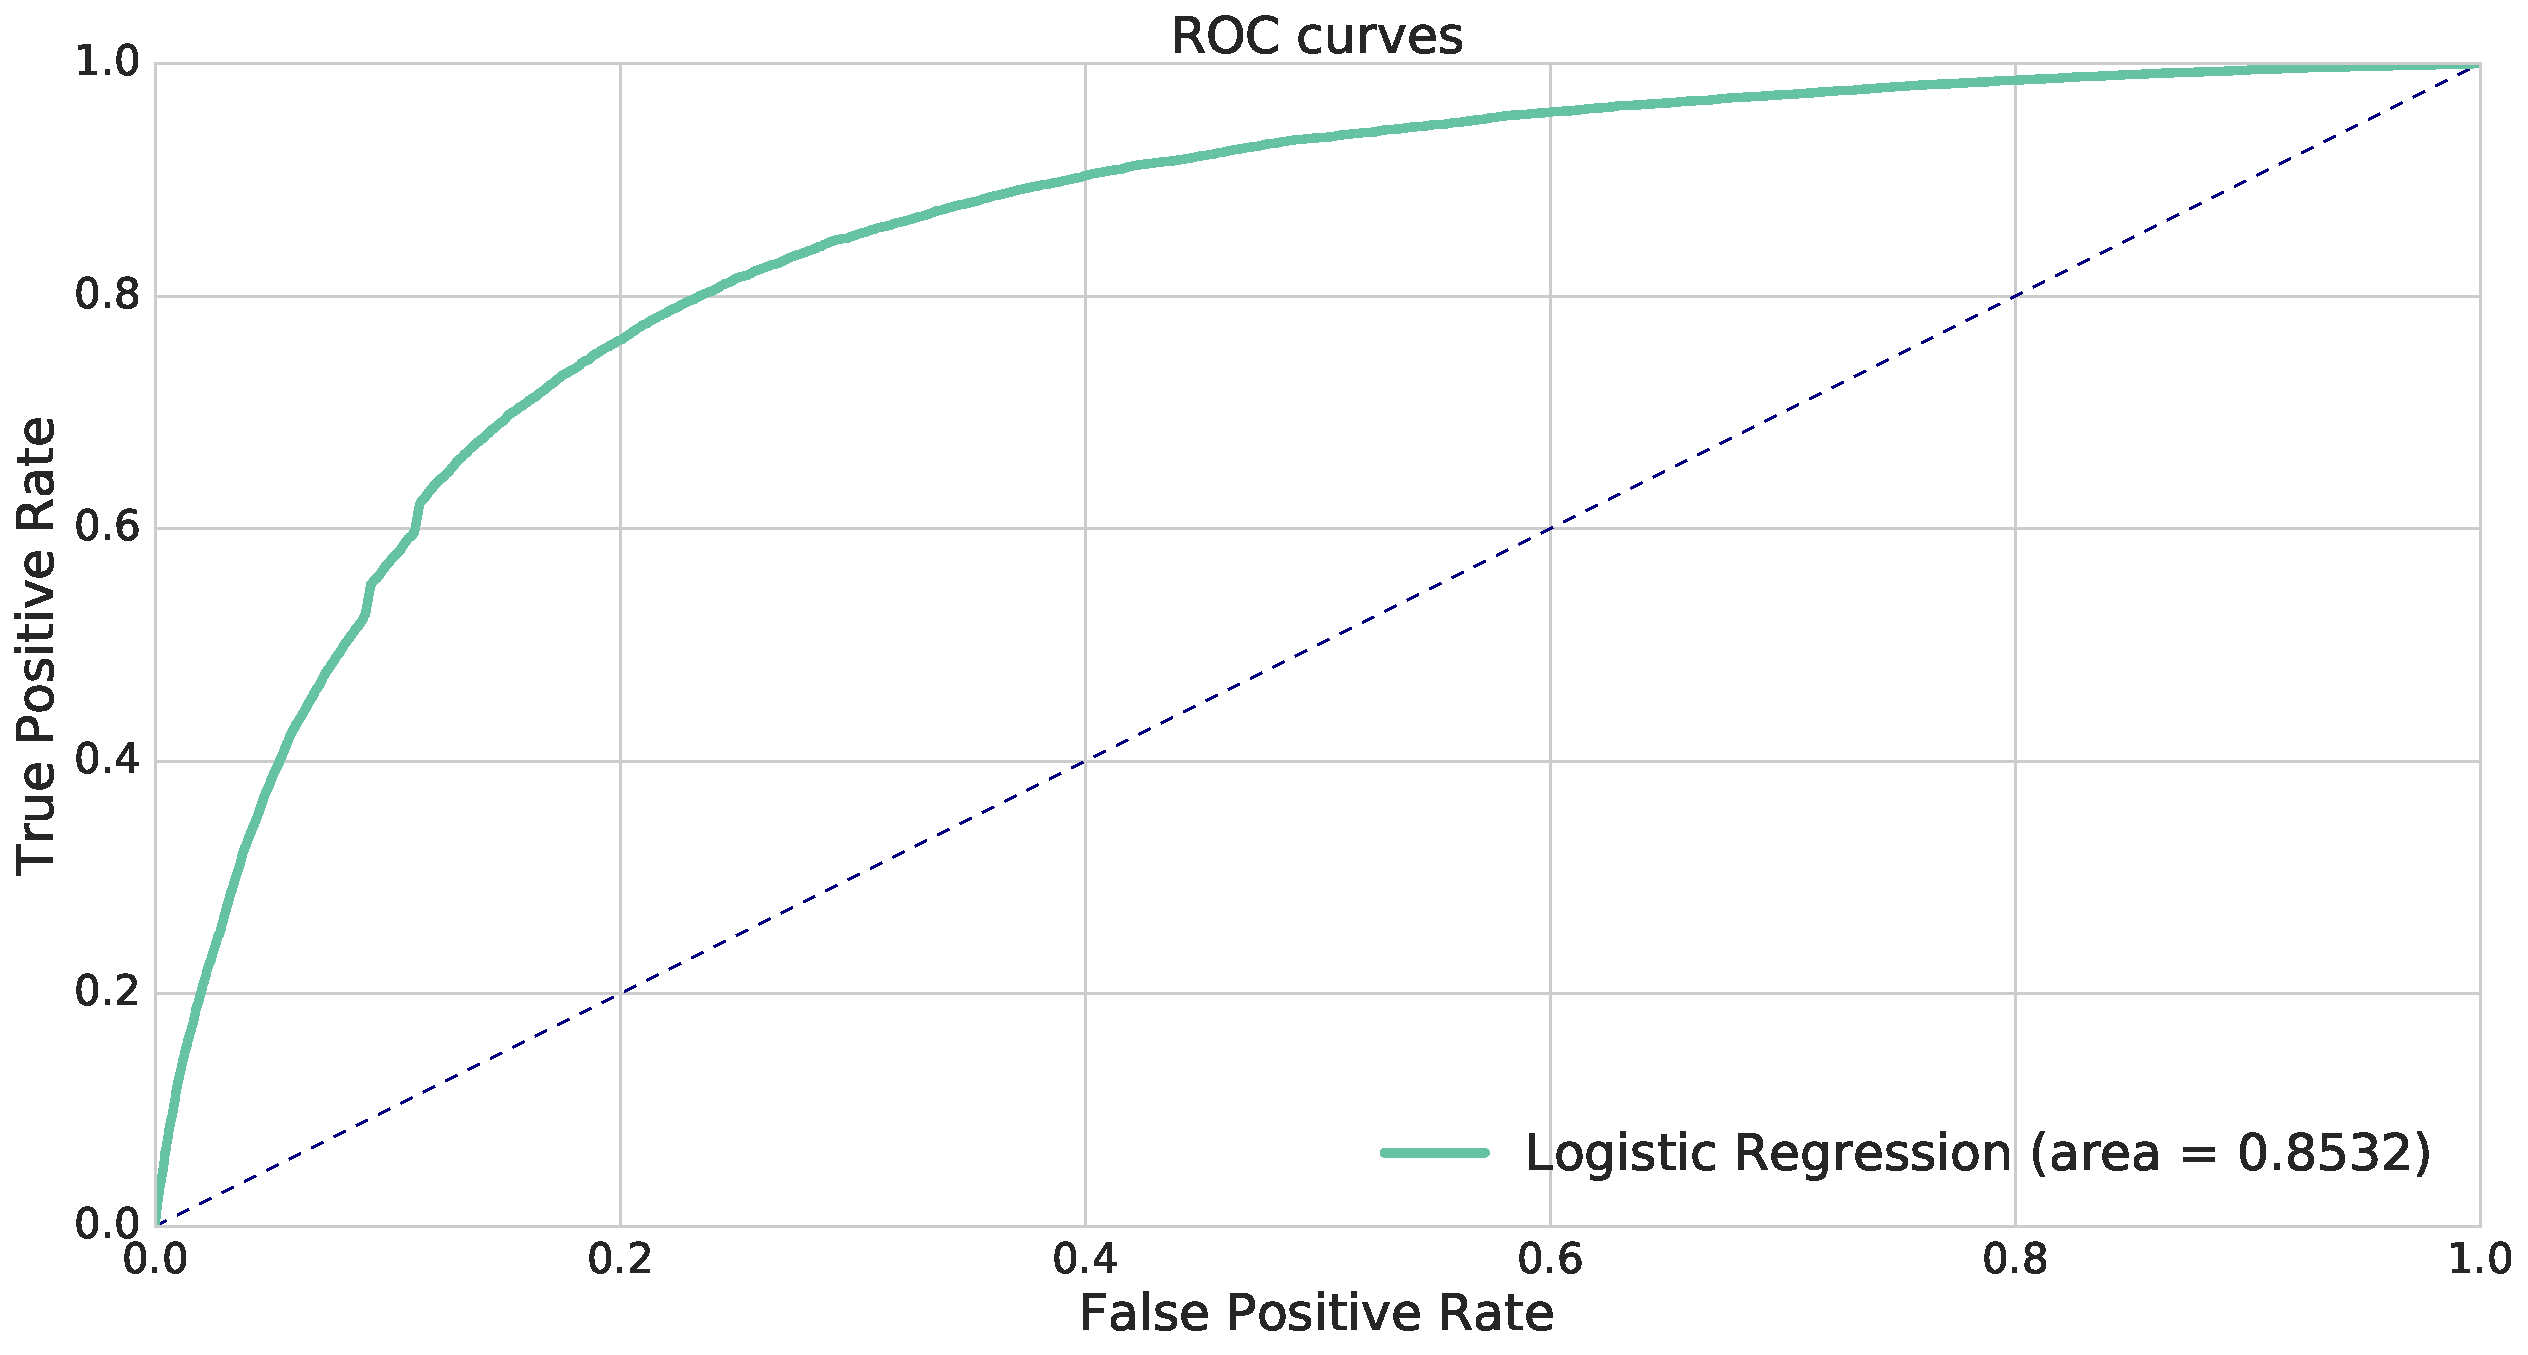
\includegraphics[width=1.0\textwidth,keepaspectratio]{figures/roc_example.pdf}
    \caption{An example of a ROC curve}
    \label{fig:roc_example}
\end{figure}

A good classifier would score values close to the upper-left corner of the plot, where the point (0,1) represents a perfect classifier with 100\% TPR and 0\% FPR. On the other hand, an algorithm that outputs a curve alongside the diagonal where TPR and FPR are almost the same at different threshold levels can be considered close to a random guess, like the flip of a coin. A classifier would underperform if its scores are closer to the bottom-right corner of the plot, however this result can always be mirrored by updating the model to simply invert the positive and negative labels of the classified samples.

ROC curves can be used to compare the performance of different models by measuring the \emph{area under the curve} (AUC) of its plotted scores, which ranges from 0.0 to 1.0. The greater this area, the better the algorithm is to find a specific feature. Moreover, models with an area close to 0.5 can be assumed to perform not much better than random guess, since this is the total area under the diagonal line. The AUC can also be interpreted as the probability of a randomly picked positive sample is ranked higher by the model when compared to a randomly picked negative case.

\subsection{Precision-Recall Curves}

While ROC curve is the most commonly used method for evaluating the performance of a classifier, it still fails to capture the true quality of the model when data is severely sparse. For any heavily skewed dataset, predicting the negative majority correctly can be accomplished easily, however the same cannot be said about the rare positive class. Since ROC curves utilizes the false positive rate calculated using the large number of true negatives, the plot may give the idea that the model is doing quite well, while failing to show its ability to predict the positive class. 

Visualizing the precision plotted against its recall value may be more informative when dealing with sparse data. The \emph{precision-recall curve} is the visualization tool that accomplishes exactly that, for every threshold value, the recall (commonly the x-axis) is plotted against its precision (the y-axis). 

\autoref{fig:prc_example} shows an example a precision-recall curve plotted for the same data from \autoref{fig:roc_example}, however focusing only in the churning class which is the focus of this study. Here we can clearly see how the precision is affected by an skewed dataset: even if our model manages to have only a small fraction of false positives, since they are many the precision will quickly be reduced.

\begin{figure}[h]
    \centering
    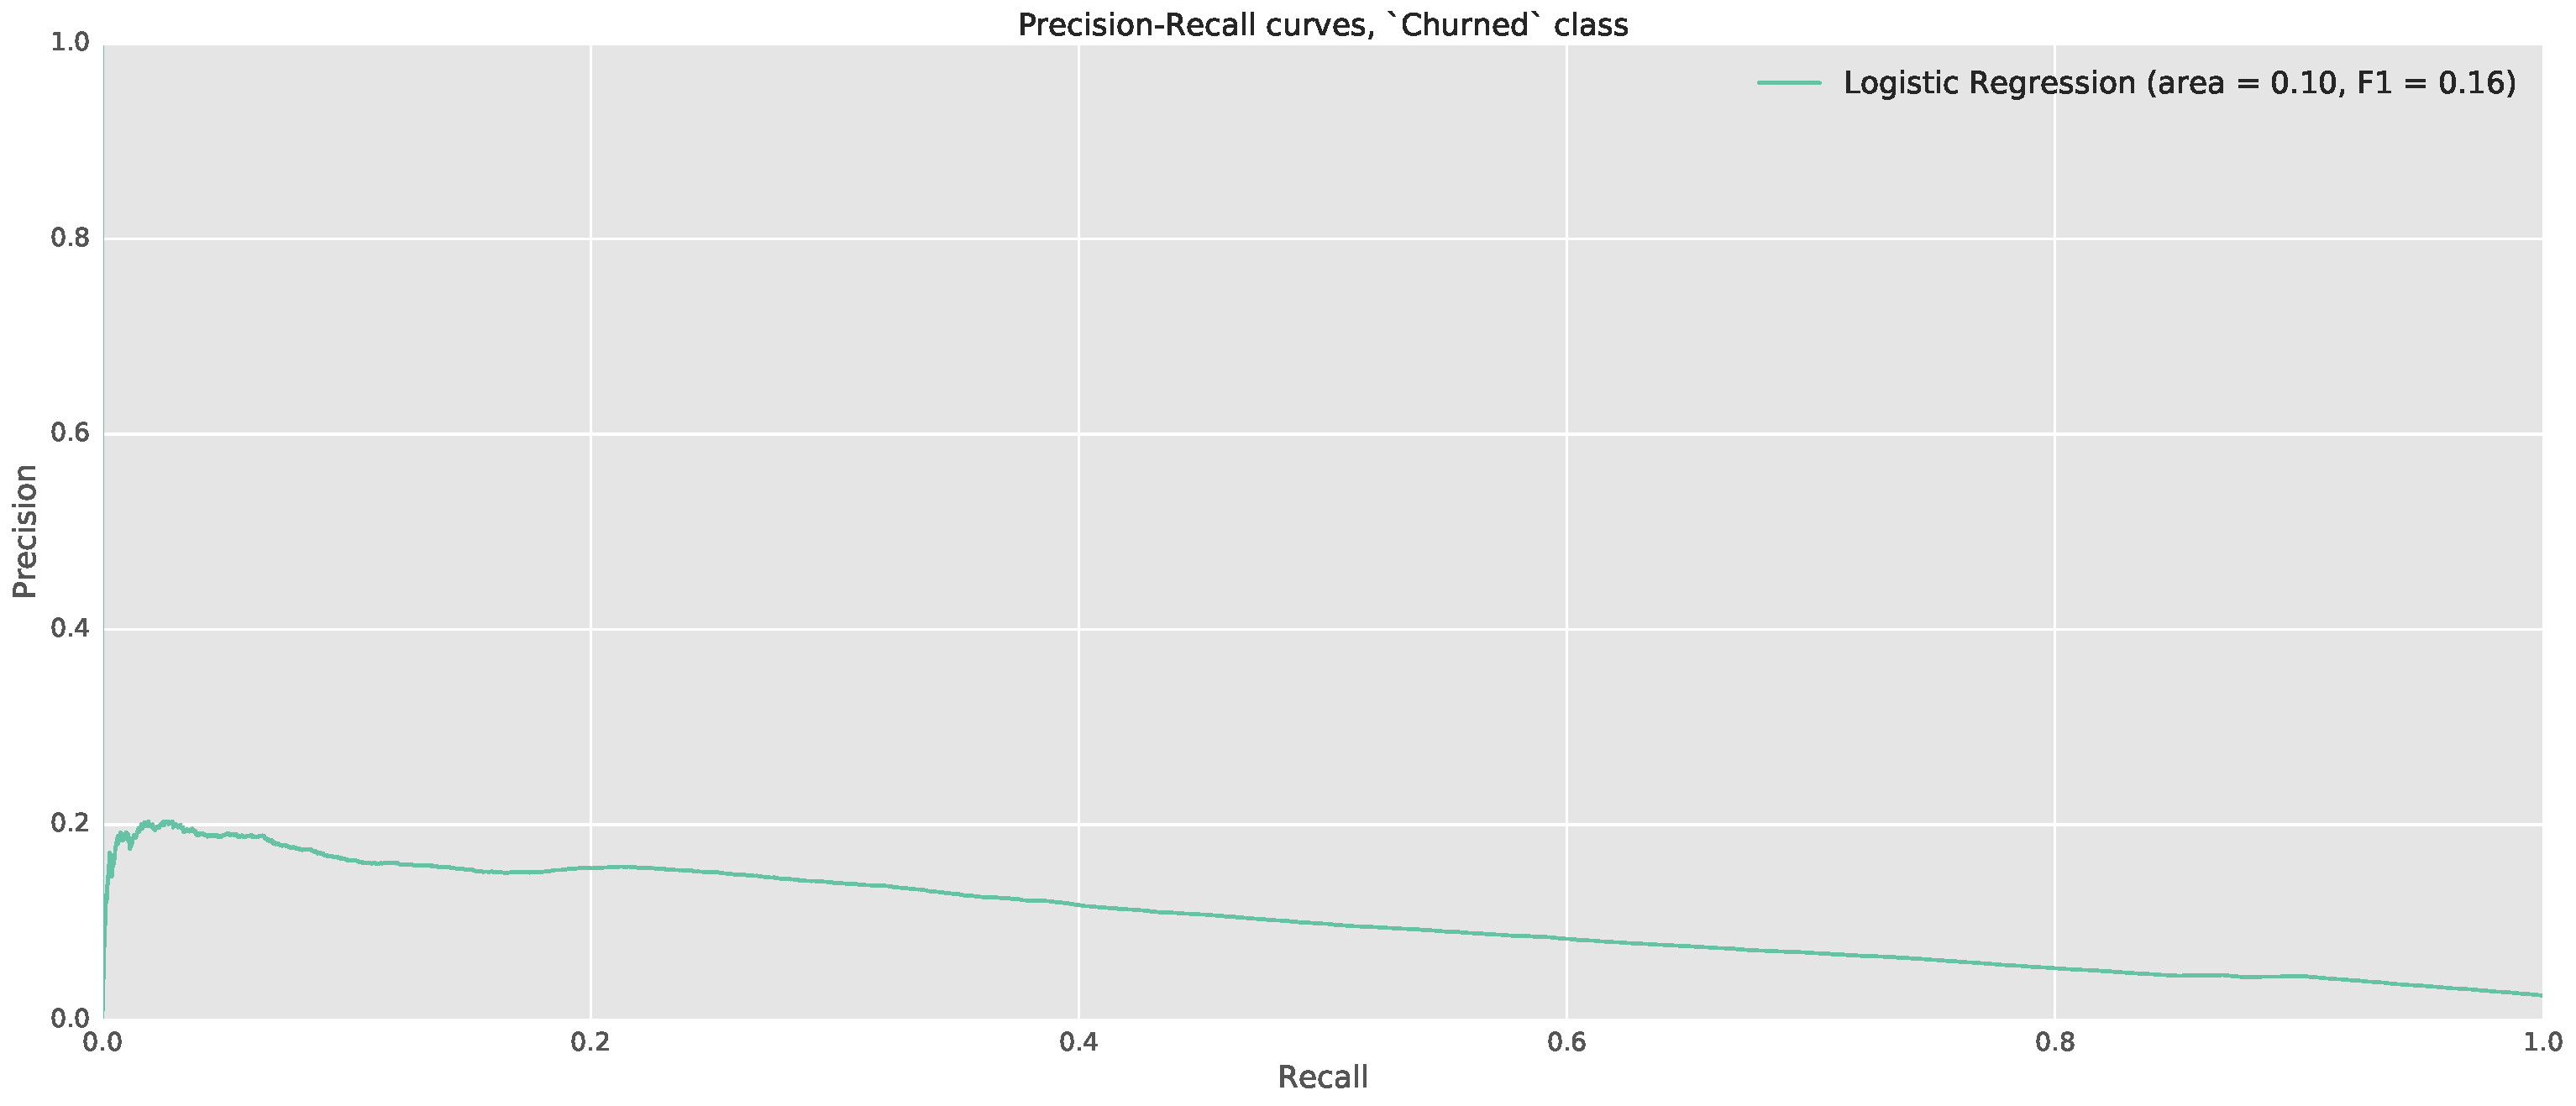
\includegraphics[width=1.0\textwidth,keepaspectratio]{figures/prc_example.pdf}
    \caption{An example of a precision-recall curve}
    \label{fig:prc_example}
\end{figure}

Similarly to ROC curves, the area under the line correlates to the overall quality of the classifier: values closer to 1 indicates that a model has high precision and recall for every different tested threshold.  The balance between precision and recall can be manipulated by changing the threshold value: if we want to increase the recall, simply using a lower threshold will yield an increase in the number of true positives, at the cost of lower precision.

\section{Software and Libraries}

The experiments on this thesis project were only made possible by utilizing well known open-source software libraries for data processing and machine learning. The recurrent LSTM models were implemented in Keras\citep{chollet2015keras}, a high-level deep learning wrapper library written in Python.  Tensorflow\citep{abadi2016tensorflow}, a library for numerical computation using data flow graphs created by Google, was used as a backend for Keras. Random forests and logistic regressions models, as well as  the procedures for handling cross-validation and hyperparameter search, were implemented on Scikit-Learn\citep{scikit-learn}, a Python module for machine learning. The random undersampling was performed using a modified version of a library called Imbalanced-Learn\citep{lema2017imbalanced}, a Python package that offers several re-sampling techniques for imbalanced datasets. 

\chapter{Results and Discussion}

\epigraph{Talk is cheap. Show me the code.}{\textit{Linus Torvalds}}

This chapter will be dedicated to detail the experiments performed in this project, while also visualizing and reasoning over the obtained results.

The experiments on this project aim to verify how the performance of current models used for predicting churn compares to a newer approach like LSTMs, and also explore how can we influence the scores of our predictor by changing different aspects of the input data. The experiments in this project are:

\begin{itemize}
\item Comparing LSTMs to baseline models commonly used for churn prediction
\item Changing the size of the prediction and observation windows
\item Exploring how the class balance between churning and retaining users influences performance
\item Verifying if reducing the dimensionality of the data can increase the scores of the predictor models 
\end{itemize}


 As to avoid overwhelming the reader with data, the main results will be presented only, while the more extensive data can be thoroughly explored in \autoref{chap:add_results}. Following are some details regarding all experiments.

\begin{itemize}
\item The precision, recall and F1-score metrics were all obtained by thresholding the output scores to 50\%, which makes no assumption of whether the provider would rather decrease precision in favor of recall or vice-versa. Precision-recall and ROC curves plot however its corresponding metrics against all possible thresholds.
\item All experiments undersample the training data to a 1-to-1 ratio between churning and retaining users, unless this is a parameter being currently tested.
\item Unless explicitly stated, the dataset being used will be composed 56 days of observation window size and 30 days of prediction.
\item Random forest and logistic regression were trained using the SPTD version of the dataset defined in \autoref{sec:timewindows},  while LSTM was trained using MPTD.
\end{itemize}

\section{LSTM vs. Baseline Models}

In this experiment, our goal is to test the performance of the LSTM model compared against the current state of the art in churn prediction. The pilot study has revealed that logistic regression and random forests are algorithms that are still fairly used in the industry and academia.

All three models were trained on the on the dataset composed of 56 days of observation time and 30 days of prediction, where undersampling was performed on the training data as to have an equal number of churners and retainers.

\begin{table}
\centering
\begin{tabular}{llrrrr}
\toprule
     &          &  F1-Score &    PR AUC &  Precision &    Recall \\
\midrule
\multirow{2}{*}{LSTM} & Retained &  \textbf{0.898539} &  \textbf{0.994353} &   \textbf{0.992256} &  \textbf{0.820997} \\
     & Churned &  \textbf{0.169514} &  0.184844 &   \textbf{0.095604} &  \textbf{0.747048} \\
\cline{1-6}
\multirow{2}{*}{Random Forest} & Retained &  0.895238 &  0.994219 &   0.991906 &  0.815740 \\
     & Churned &  0.163607 &  \textbf{0.196442} &   0.092014 &  0.737191 \\
\cline{1-6}
\multirow{2}{*}{Logistic Regression} & Retained &  0.830156 &  0.992835 &   0.991119 &  0.714172 \\
     & Churned &  0.114696 &  0.103541 &   0.062114 &  0.747341 \\
\bottomrule
\end{tabular}
\caption{Metrics for the LSTM vs. baseline experiment}
\label{tab:temporal_static}
\end{table}

The results for this experiment shows that LSTM has the best overall performance of the evaluated models for almost all metrics in \autoref{tab:temporal_static}. It must be noted however that the difference to random forest is very slim, a model which is significantly faster to train and optimize. The intuition behind the surprising performance of random forests is that it can more easily learn the correlations between the data and the binary label given that proper features are engineered. On the other hand, the LSTM model performed significantly better than logistic regression in all metrics.

\begin{figure}
    \centering
    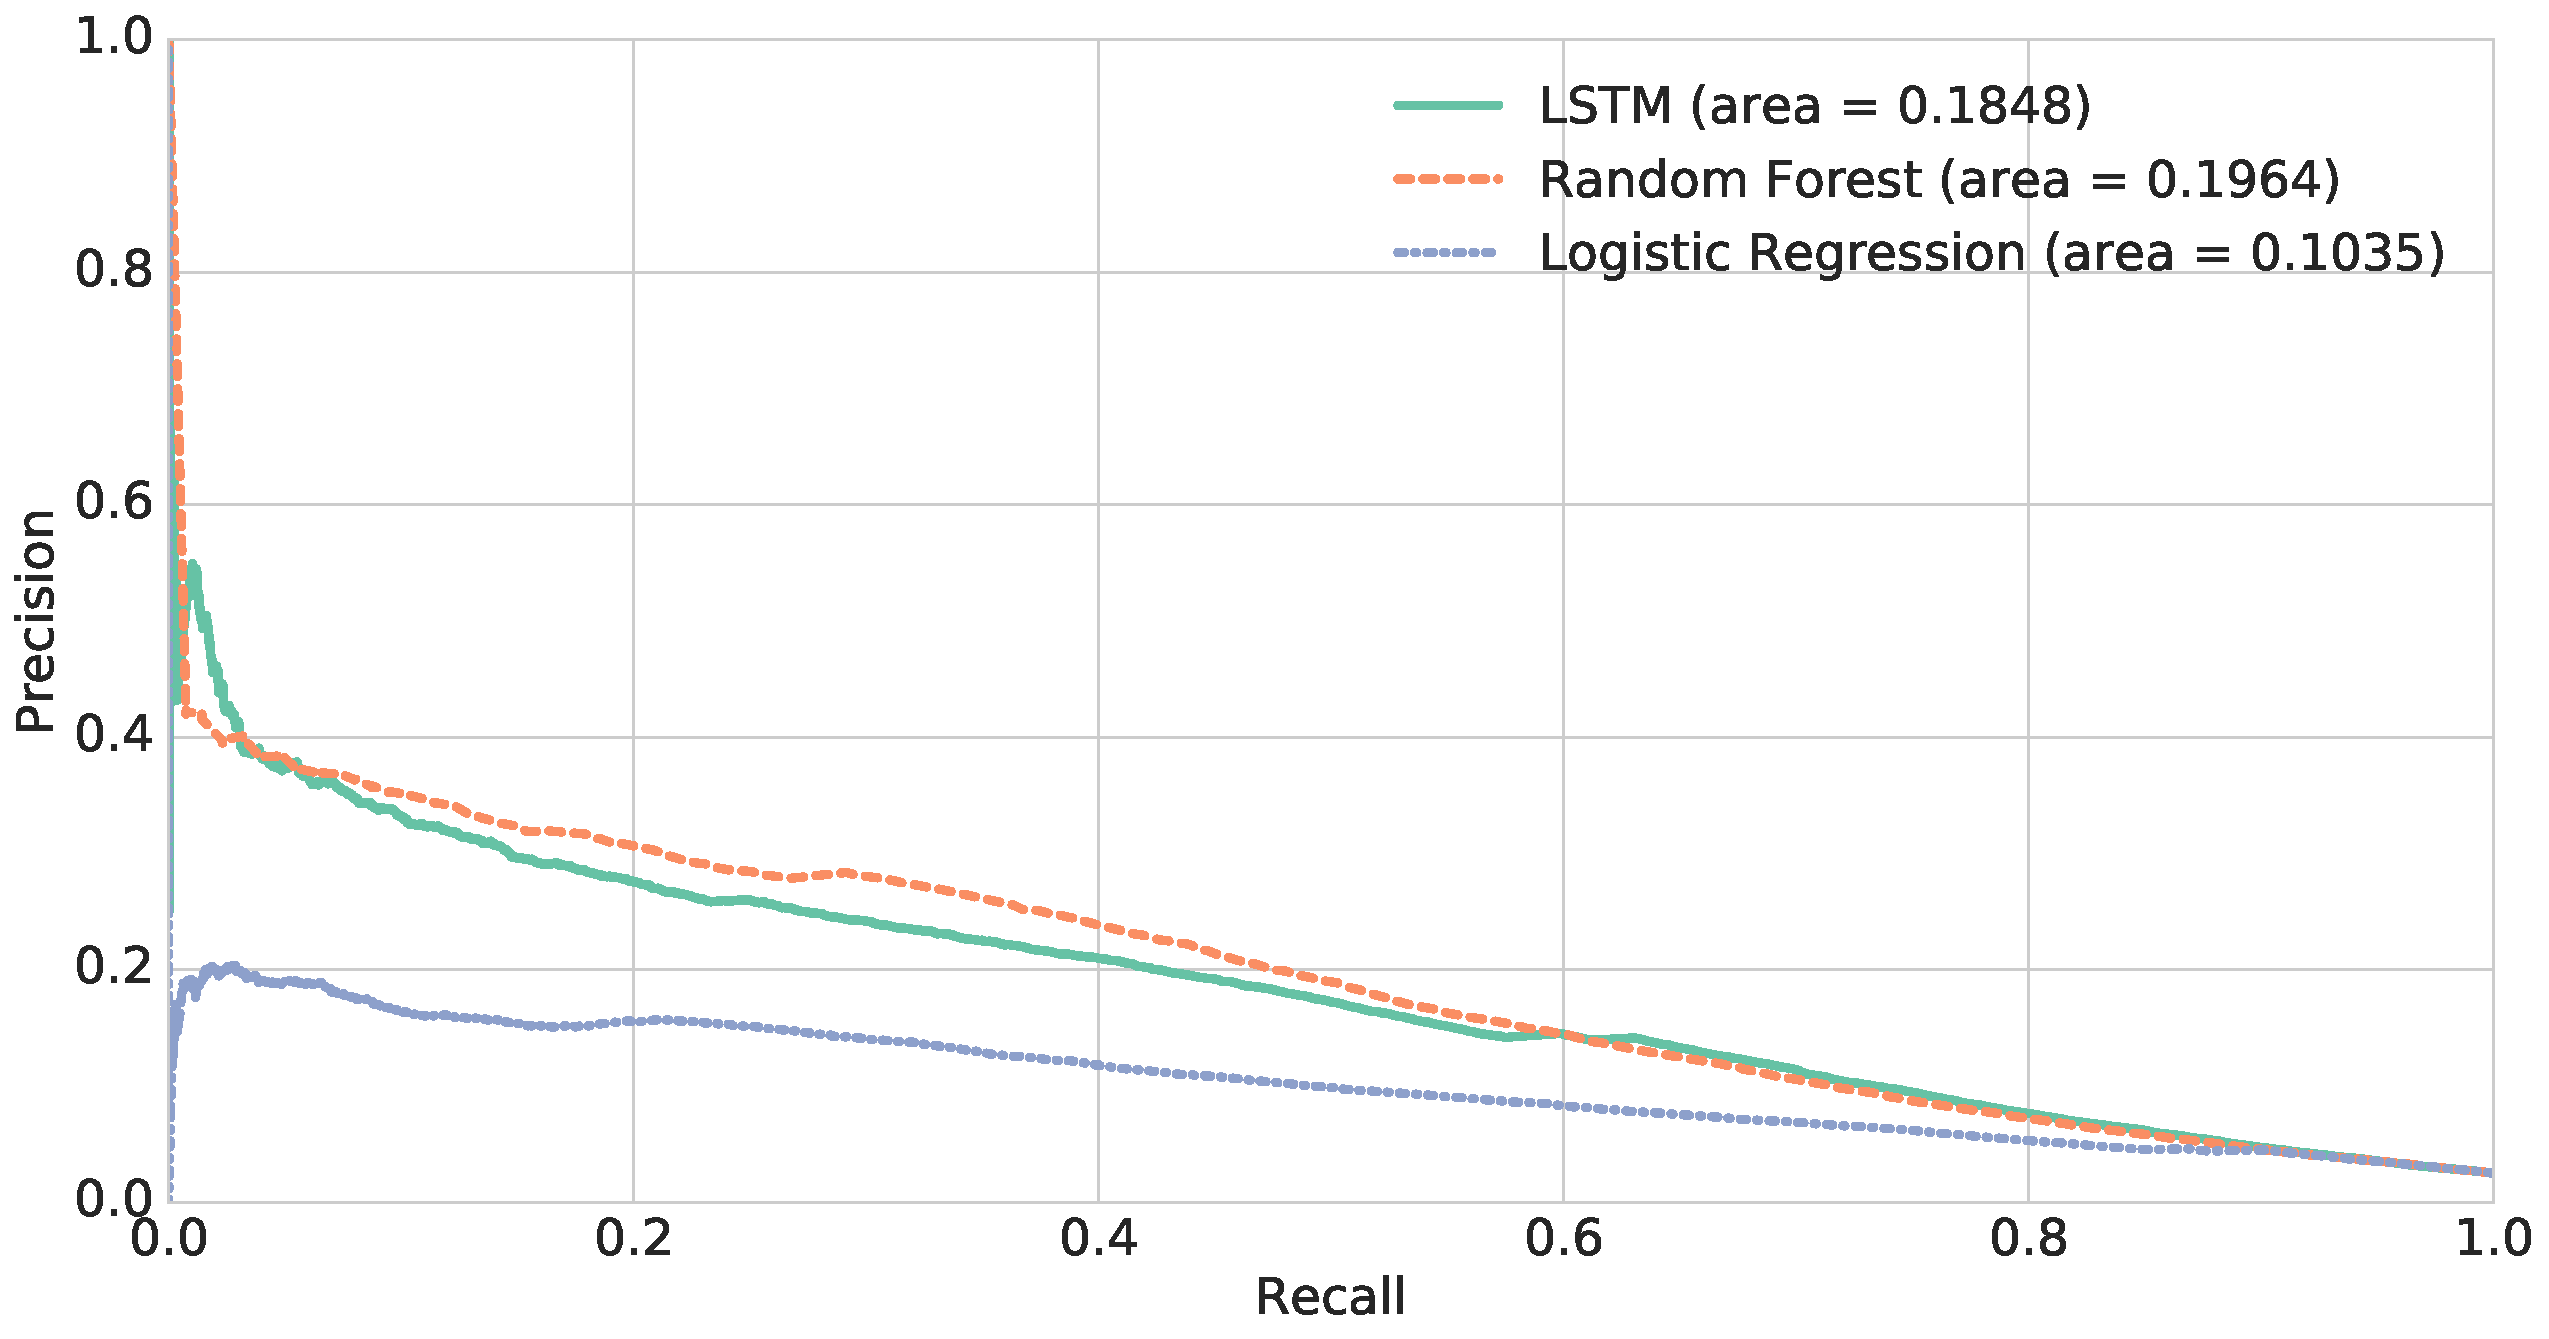
\includegraphics[width=1.0\textwidth,keepaspectratio]{figures/prc_temporal_static.pdf}
    \caption{Precision-recall curves of the churned class for the LSTM and baseline models}
    \label{fig:prc_temporal_static}
\end{figure}

\begin{figure}
    \centering
    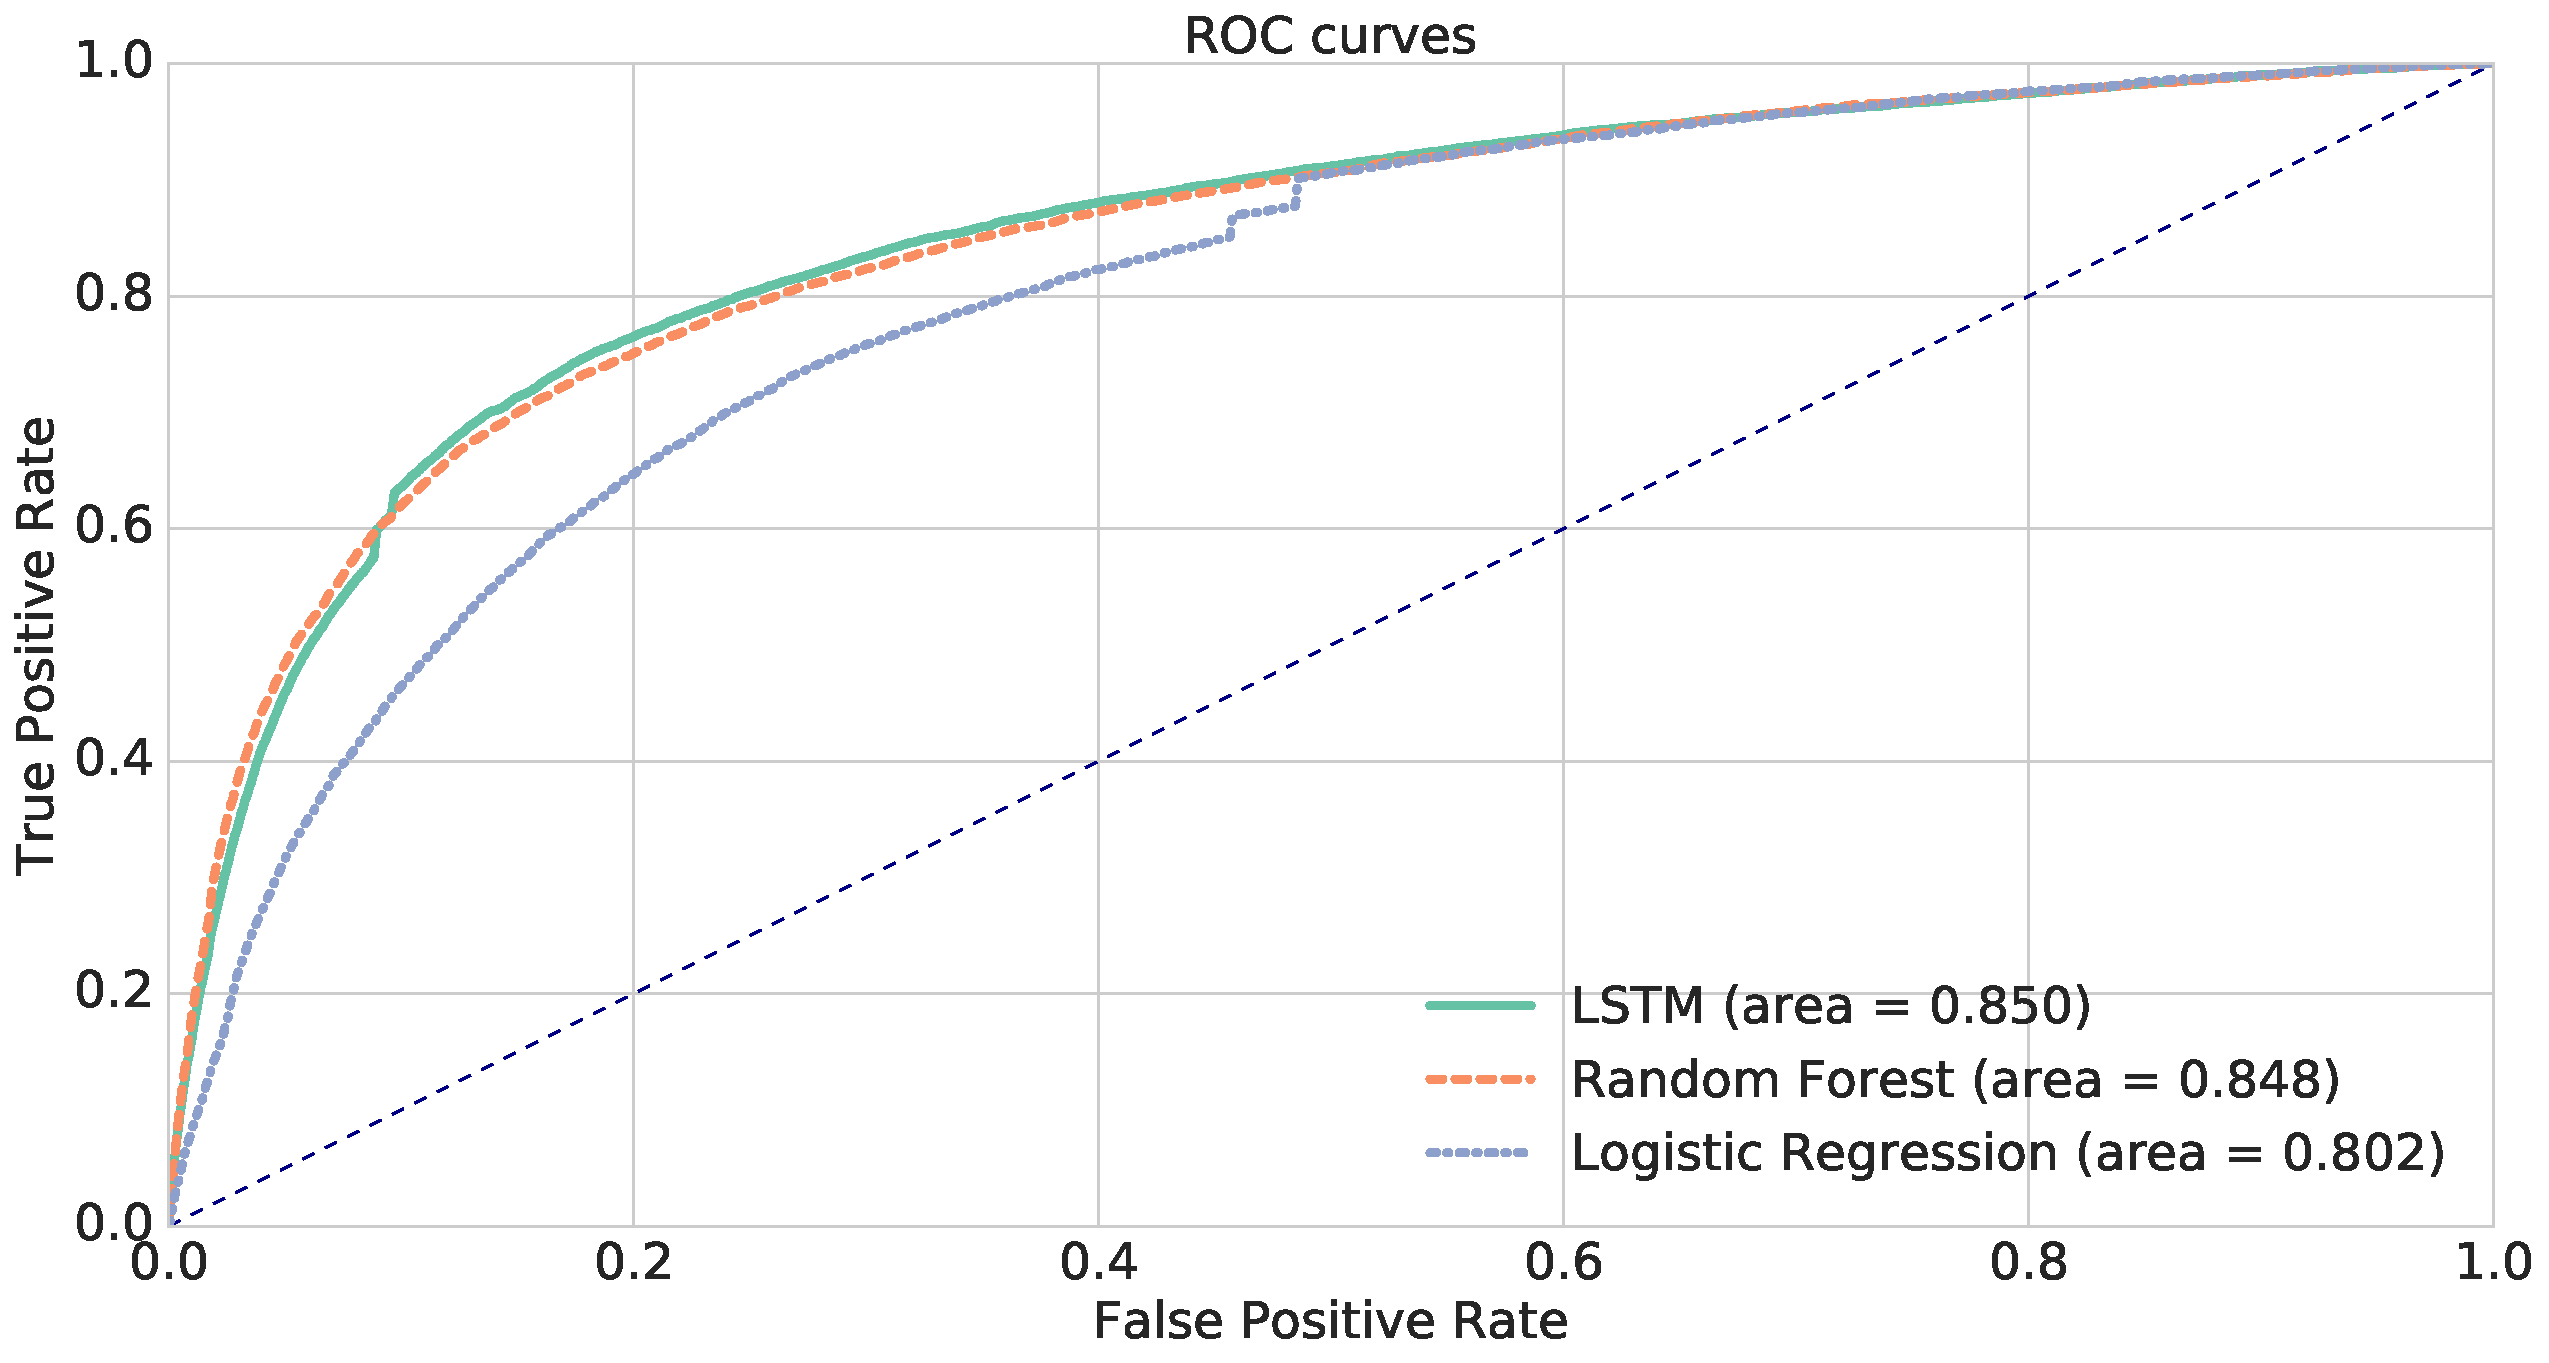
\includegraphics[width=1.0\textwidth,keepaspectratio]{figures/roc_temporal_static.pdf}
    \caption{ROC curves for the LSTM and baseline models}
    \label{fig:roc_temporal_static}
\end{figure}

\autoref{fig:prc_temporal_static} and \autoref{fig:roc_temporal_static} plots the precision-recall and ROC curves for the LSTM and the evaluated baseline models for several different threshold levels. In it it can be clearly seen how similar the metrics of LSTMs and random forests are, the curves frequently overlap along the x-axis. The gap in performance between logistic regression and the top predictors observed in the metrics table is further visualized in these plots, suggesting that this model might not be a good choice for predicting churn for this specific dataset. 


\section{Experimenting on Different Window Sizes}

The size chosen for the time windows may have an influence on the performance metrics of our trained estimators that is non-trivial to predict. Even though an intuitive guess can be made for the effect of the change, the set of values that maximizes the accuracy of the classifiers while being compliant to the company's goals and also the available computing resources is \textit{a priori} unknown. This experiment attempts to answer this question by training several models while changing the observation and the prediction window sizes, and by plotting the best score obtained for each estimator.

\Todo{More details to the time windows experiments. Add maybe a figure showing the different windows}

\subsection{Observation Window}

Increasing the size of the observation window basically means that more data is going to be used for training. It is expected that with more data, a better accuracy can be achieved, however that comes with the cost of an ever increasing training time. So the question that this experiment is exploring is how far in the user history must we train our models on as to obtain a good trade-off between accuracy and training time, a topic thoroughly explored in the work of \citep{Ballings2012}.

Our experiment involved increasing the size of the observation window by 7 days and training a model for each, evaluating the performance of each. The prediction window is made constant at 30 days, corresponding to the same period in time for all different parameters tested in this experiment. The effect of modifying the observation window size for both retained and churned classes can be seen in \autoref{fig:line_obs_window} and \autoref{fig:line_obs_window_ret}, respectively. 

\begin{figure}
    \centering
    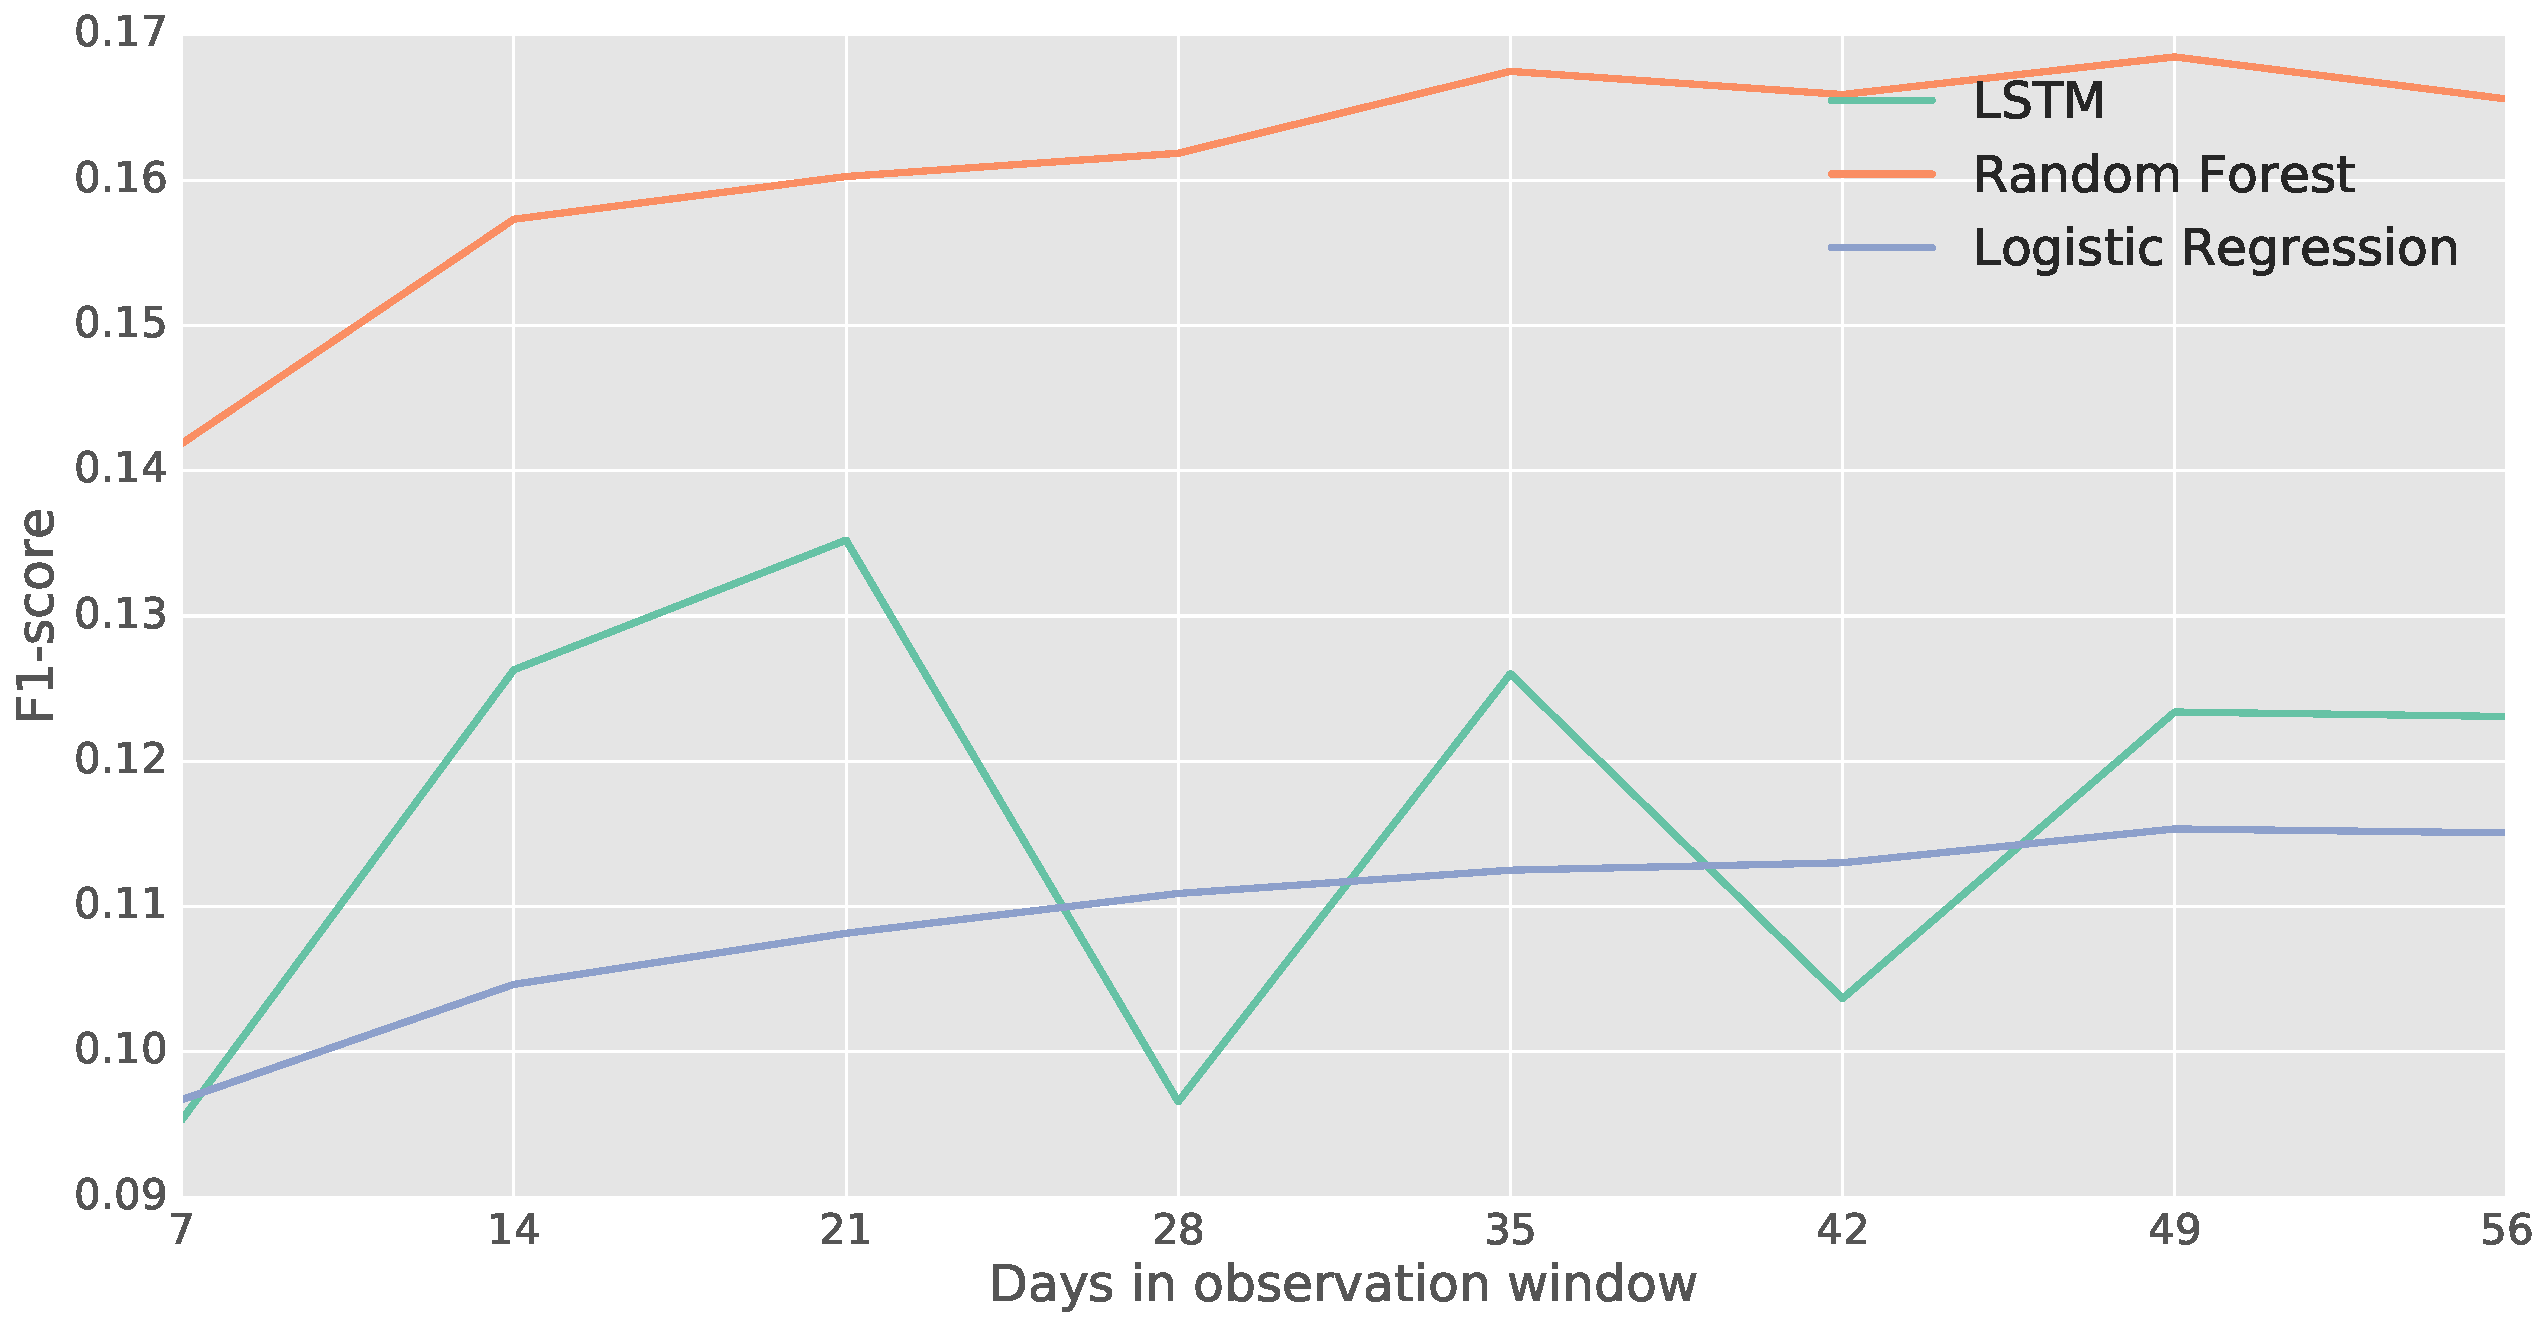
\includegraphics[width=1.0\textwidth,keepaspectratio]{figures/line_obs_window.pdf}
    \caption{F1-scores for the churned class using different observation window sizes and models}
    \label{fig:line_obs_window}
\end{figure}

\begin{figure}
    \centering
    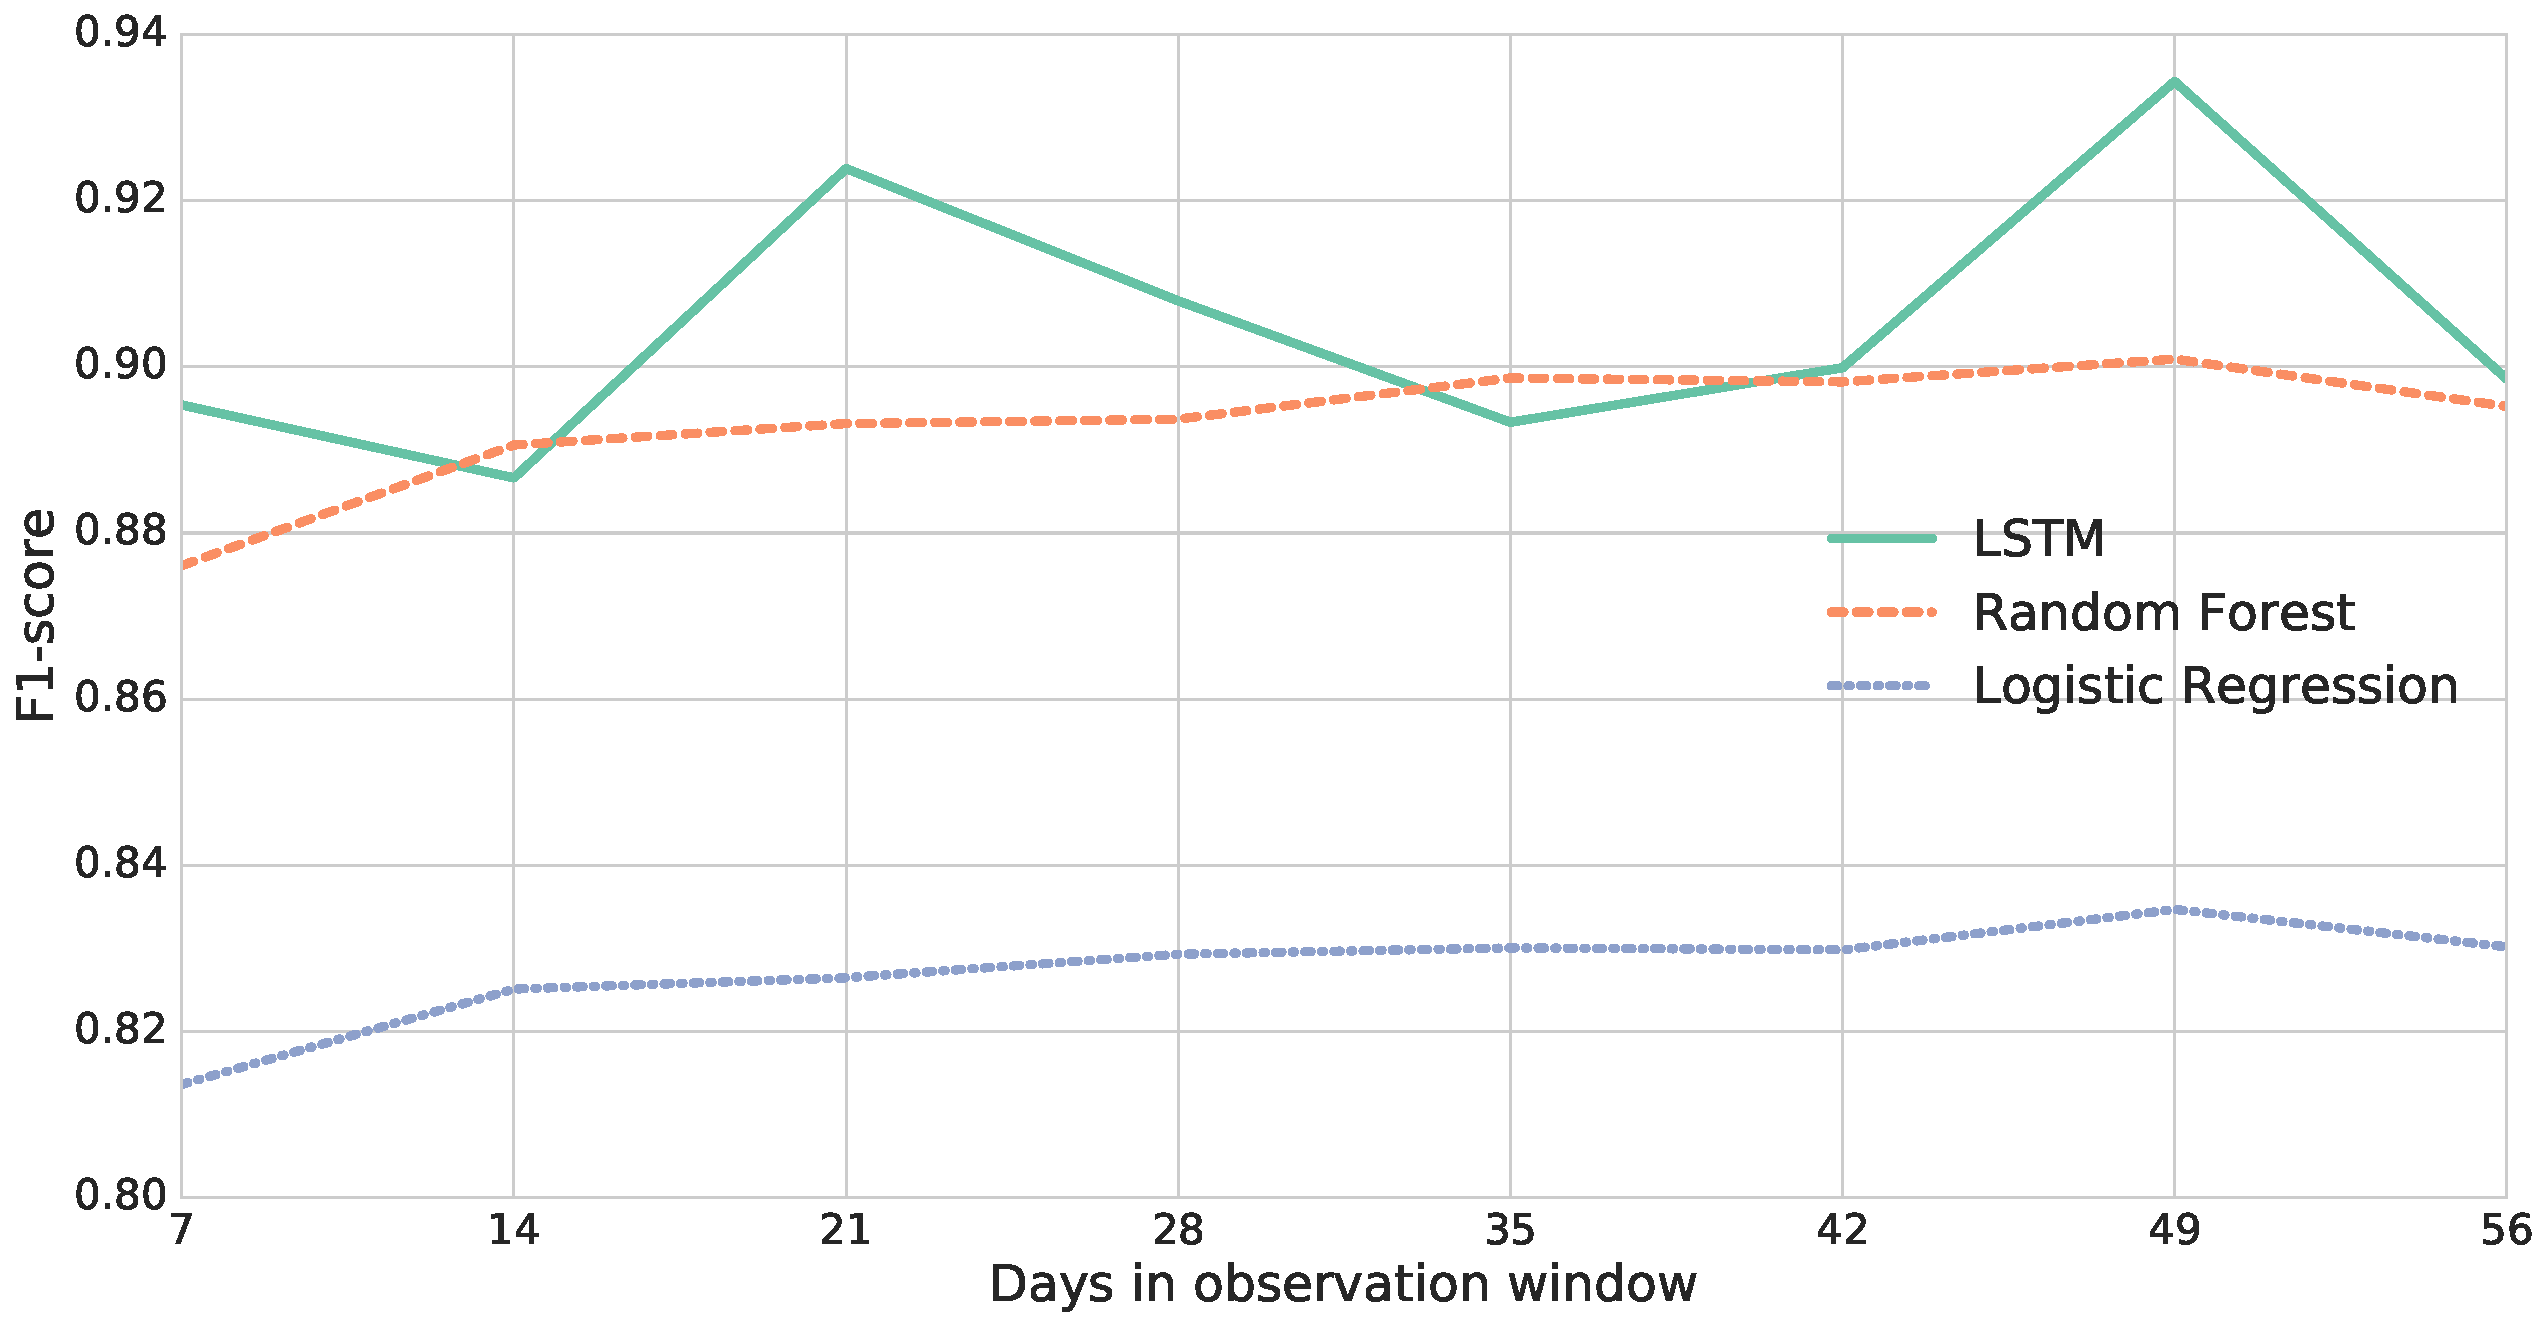
\includegraphics[width=1.0\textwidth,keepaspectratio]{figures/line_obs_window_retained.pdf}
    \caption{F1-scores for the retained class using different observation window sizes and models}
    \label{fig:line_obs_window_ret}
\end{figure}

Both the random forest and logistic regression models exhibit an increase in F1-scores when the size of the observation window is made larger, however the gain can hardly be considered significant. The LSTM model on the other hand show a rather erratic behavior, reaching its top when the window is sized at 49 days. Precision-recall curves, ROC curves and a table with all metrics for this experiment can be seen in \autoref{fig:prc_obs_window}, \autoref{fig:roc_obs_window} and \autoref{tab:obs_window}, respectively.

\subsection{Prediction Window}

Modifying the size of the prediction window indicates how tolerant we are for considering a user a churner or not. Small windows are commonly used for services lacking a formal contract between the provider and the customer, which is similar approach used in the works of \citep{Dror2012}, \citep{Runge2014} and \citep{Pudipeddi2014}. Larger prediction window sizes are often seem in "classical" service providers like the telecom industry where a contract is commonly established, an approach that is widely seem in the churn prediction literature, \citep{Khan2015} and \citep{Hassouna2015} to name a few.

This experiment involves changing the size of the prediction window in intervals of 7 days while keeping the observation window size constant in time and sized at 56 days. It is important to note that smaller window sizes means that a larger share of users will be considered churners, and due to our undersampling technique this also means that the number of samples used for training will be larger. 

The result of this experiment for the churning users can be seen in\autoref{fig:line_pred_window}. Both LSTM and random forests exhibit a good performance when the prediction window is small in size, gradually and significantly reducing its F1-score as more days are added to the window. Two reasons for this behavior can be inferred: First, smaller window means more churners, and that means more training data. Second, it is intuitively easier to predict what the user is going to do right after the observation period when compared to further days in the future. 

The same can not be said about the performance of predictor for the retaining class of \autoref{fig:line_pred_window_ret}. There is a gradual increase of the F1-score as more days are added to the window, however the difference between the highest and lowest values is considerably smaller as the one observed for the churning users. Precision-recall curves, ROC curves and a table with all metrics for this experiment can be seen in \autoref{fig:prc_pred_window}, \autoref{fig:roc_pred_window} and \autoref{tab:pred_window}, respectively.


\begin{figure}
    \centering
    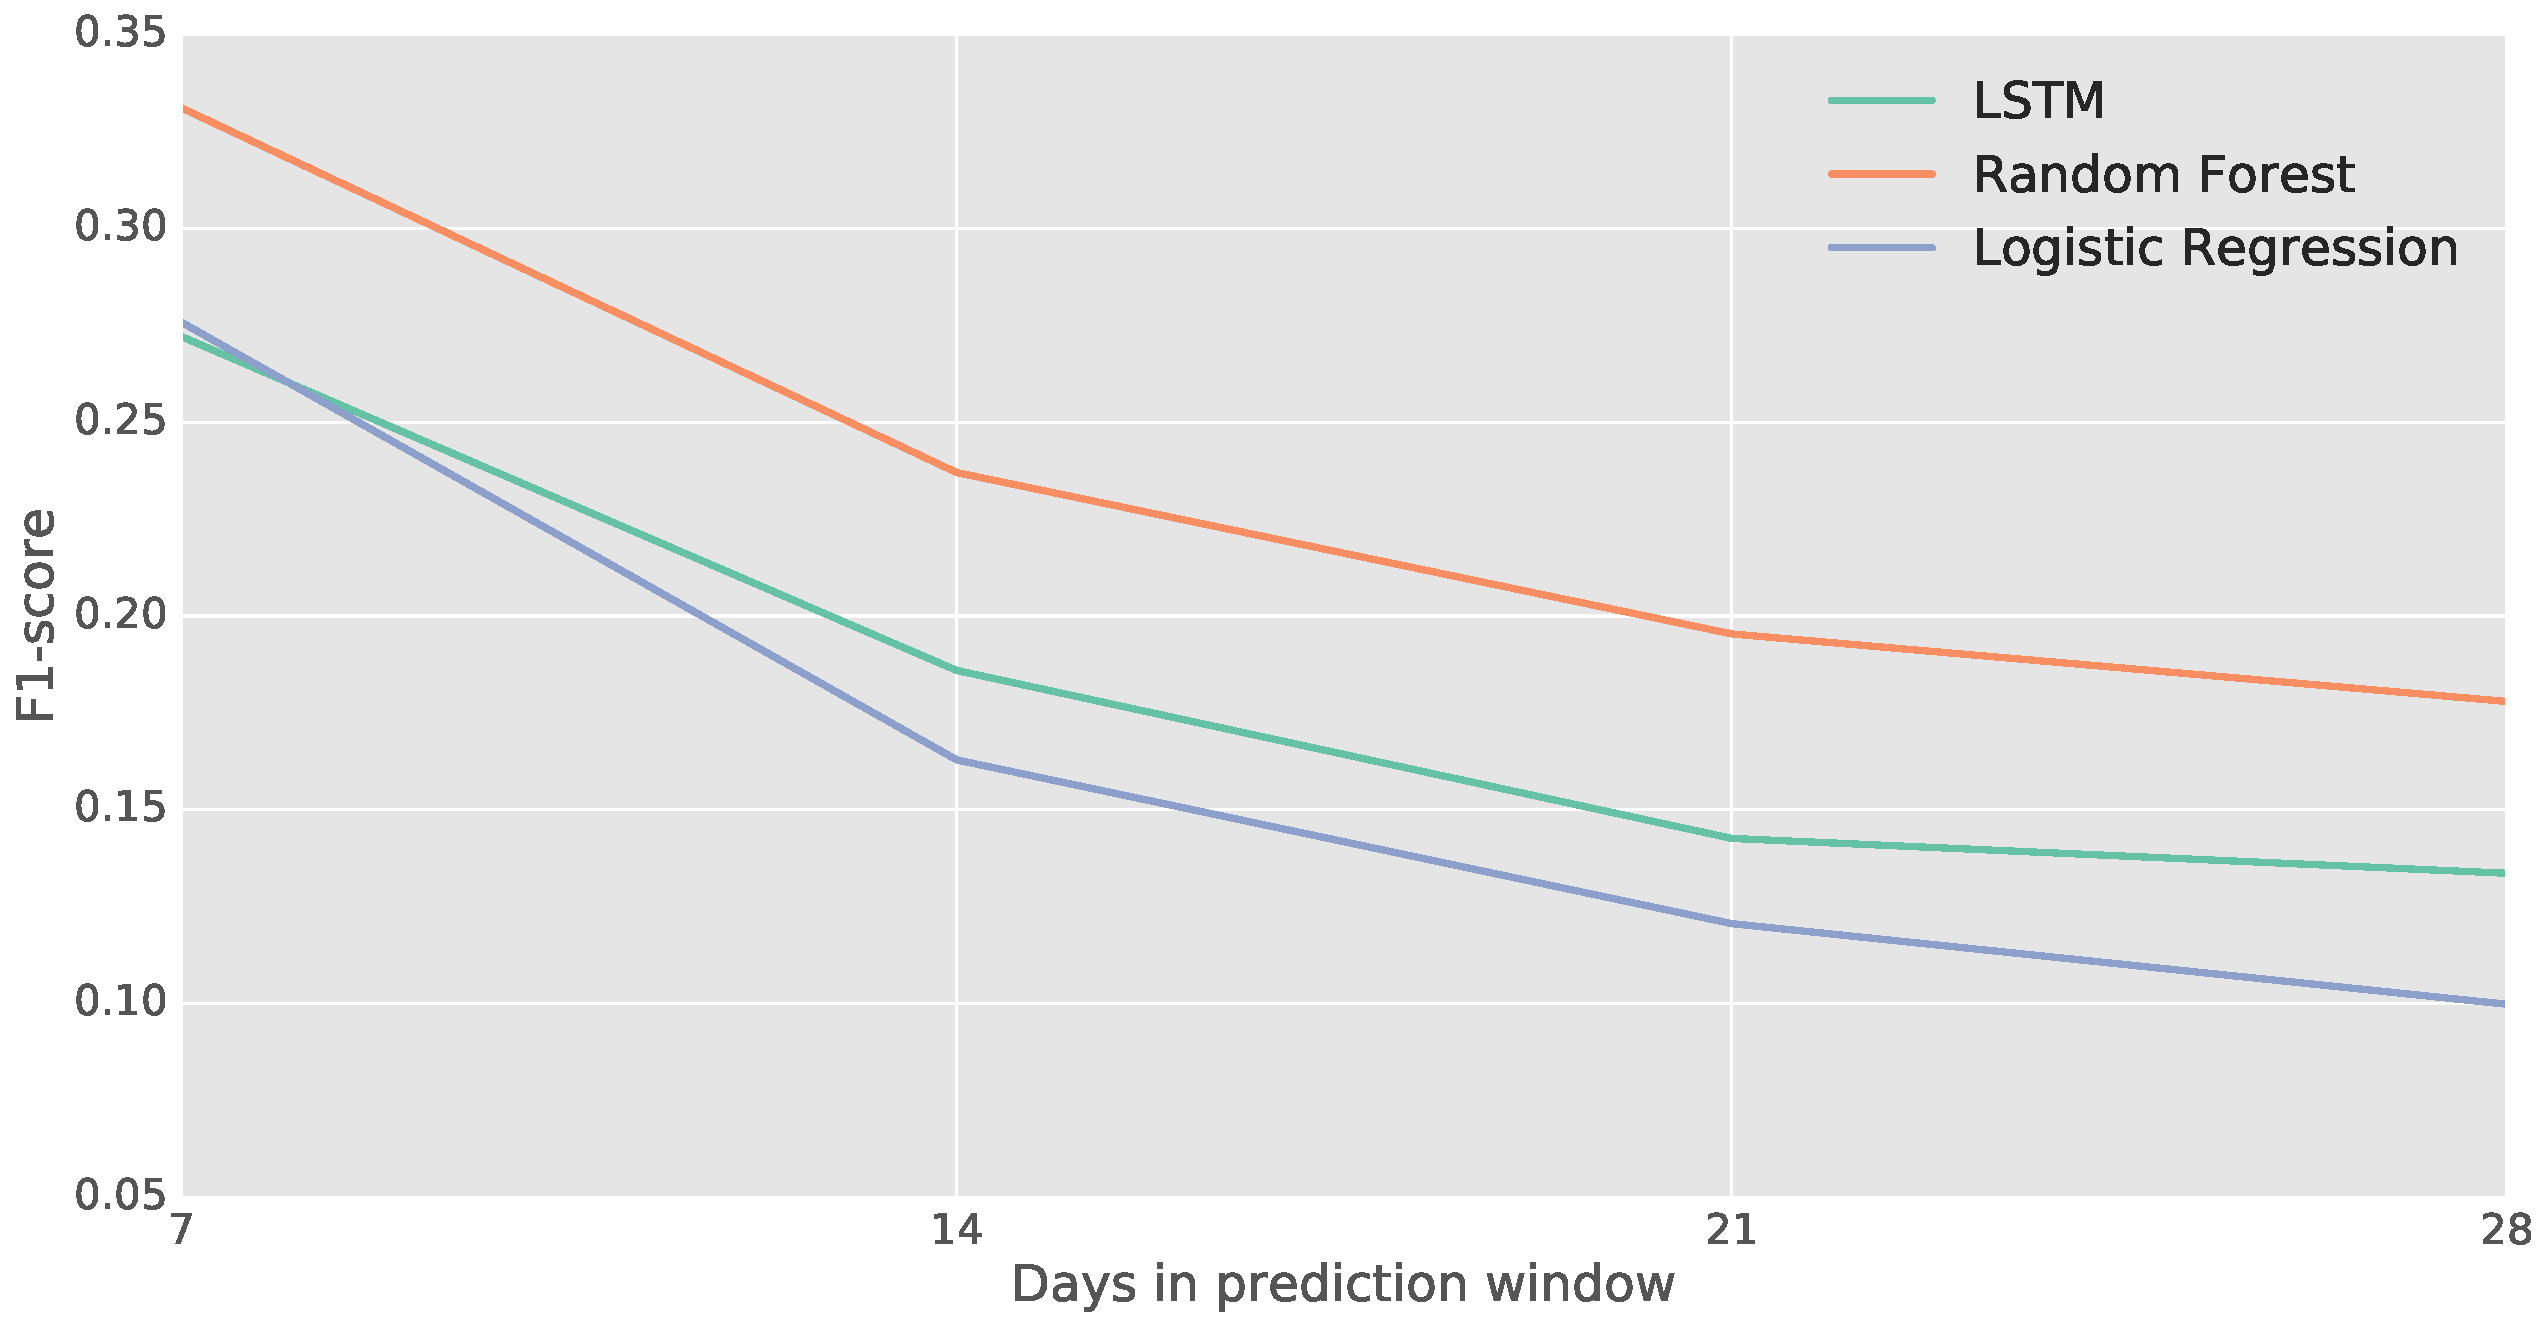
\includegraphics[width=1.0\textwidth,keepaspectratio]{figures/line_pred_window.pdf}
    \caption{F1-scores for the churned class for different prediction window sizes and models}
    \label{fig:line_pred_window}
\end{figure}

\begin{figure}
    \centering
    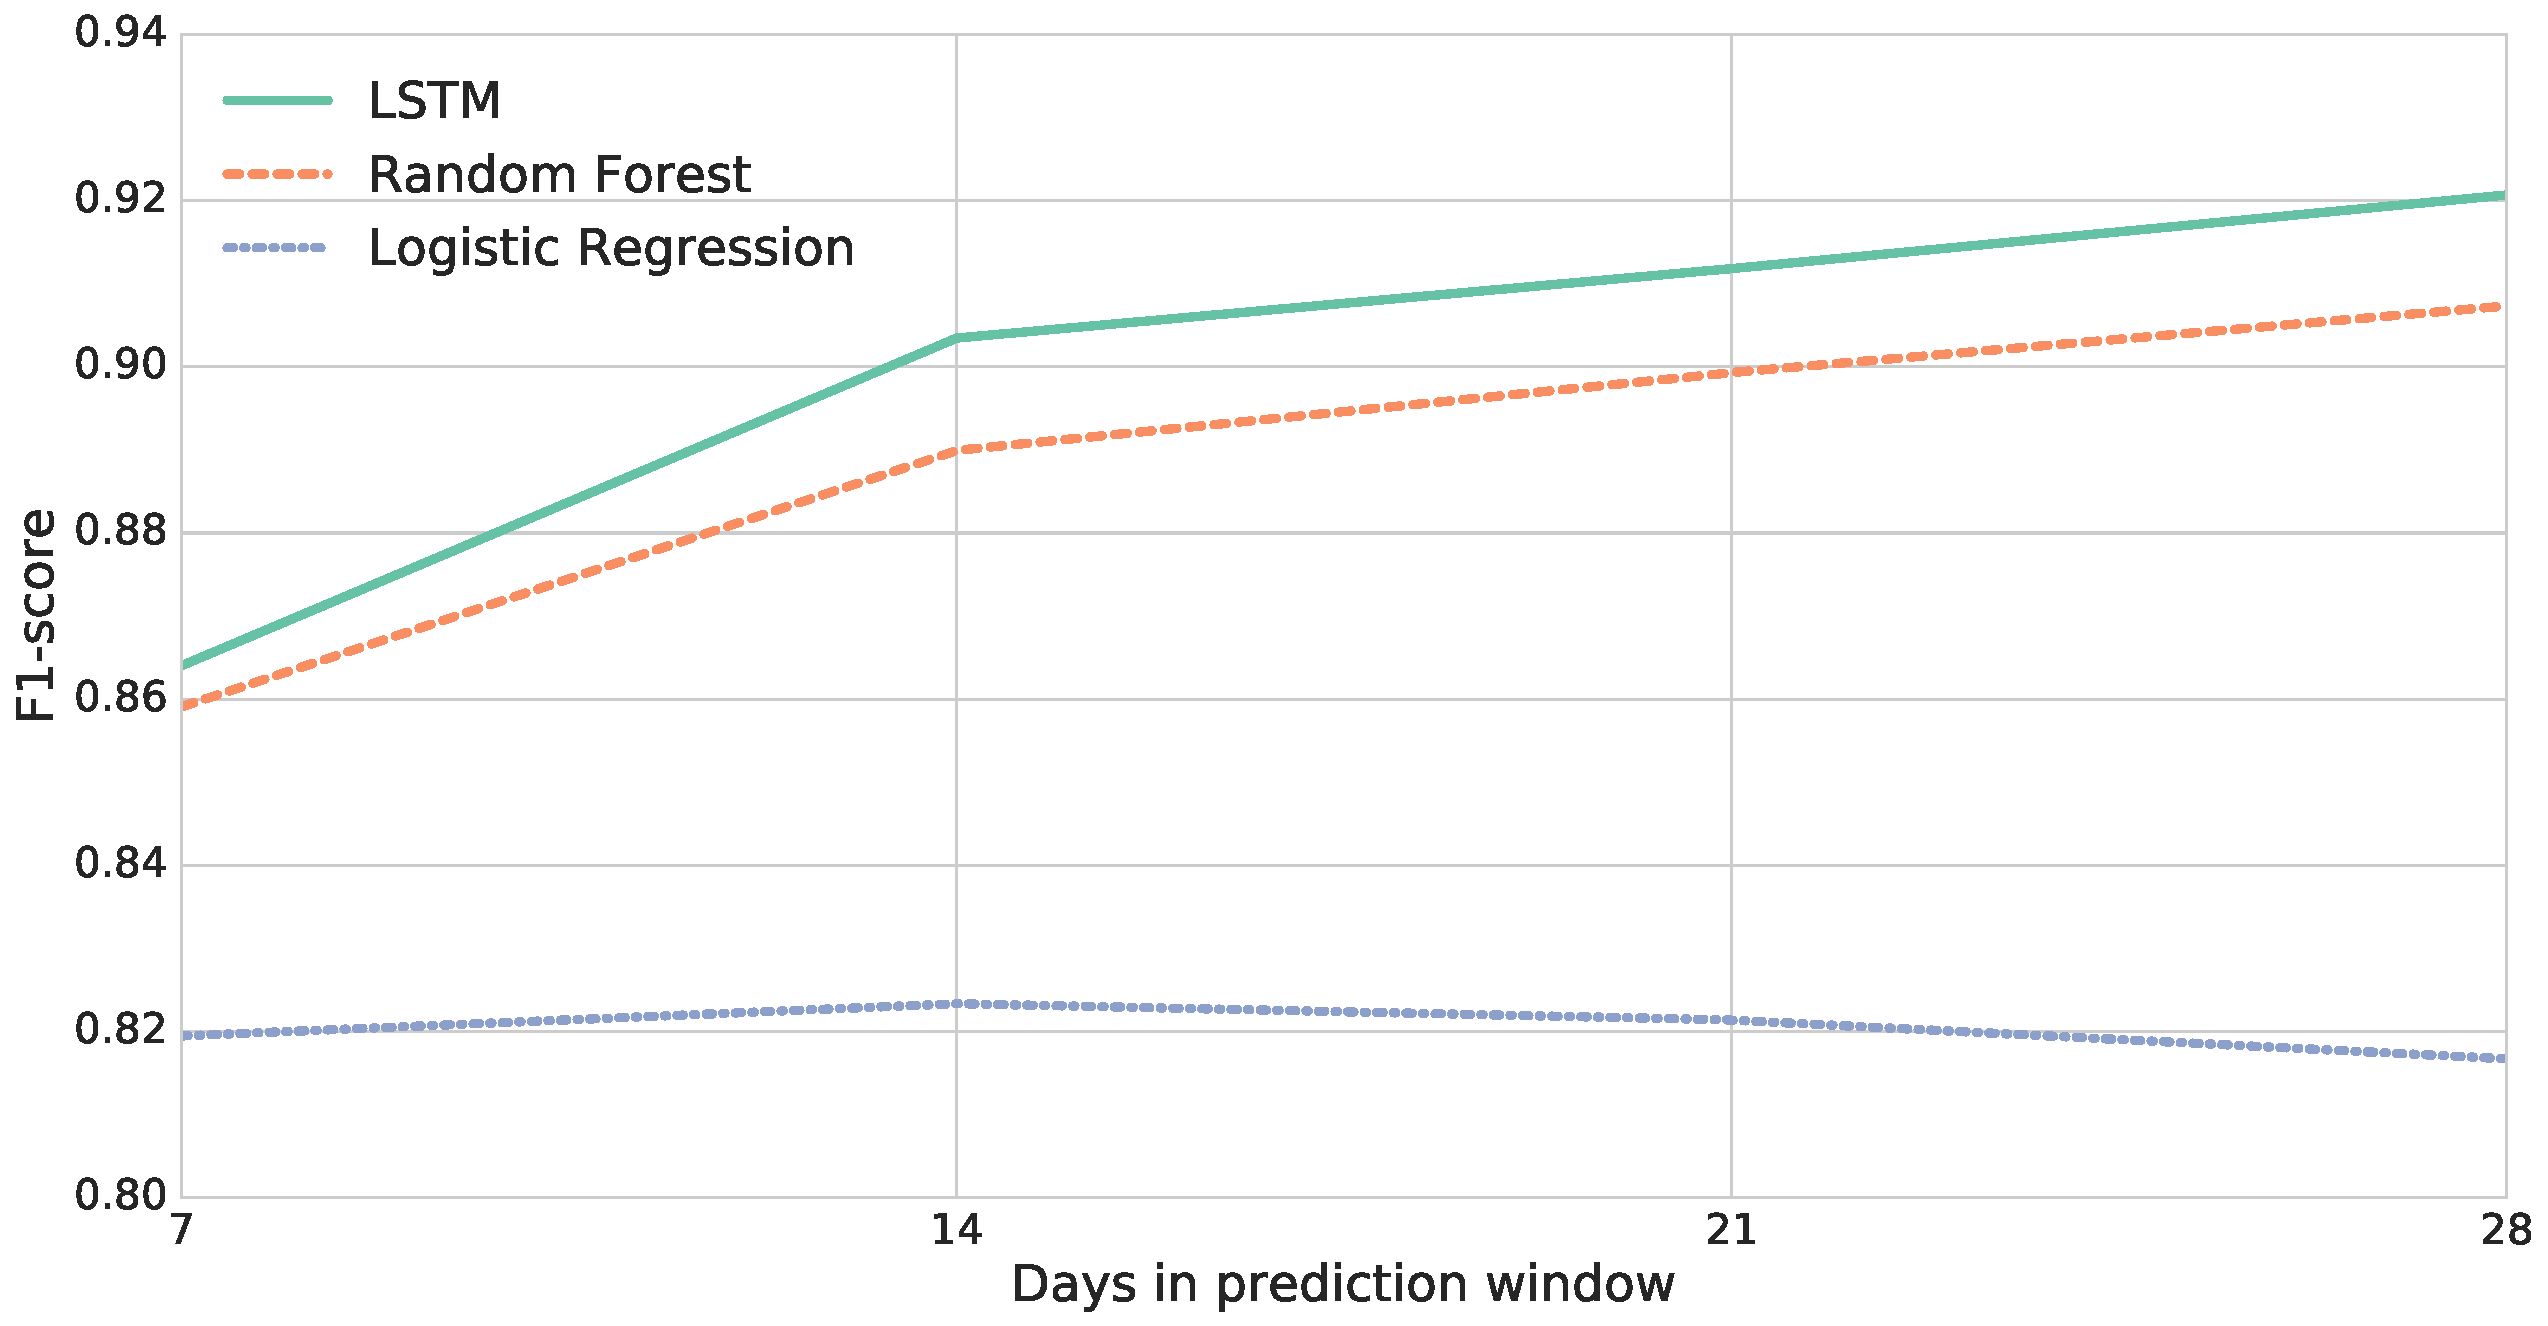
\includegraphics[width=1.0\textwidth,keepaspectratio]{figures/line_pred_window_retained.pdf}
    \caption{F1-scores for the retained class for different prediction window sizes and models}
    \label{fig:line_pred_window_ret}
\end{figure}

\section{Effect of Class Distribution}

The dataset being used for training our predictor models is heavily skewed towards the retaining class. Training models with the data in its raw form may yield an estimator that fails to capture the latent information of user behavior for the minority class, which is the one the service provider is more interested in. There is often a gain in performance when narrowing the gap between the distributions of the classes, however the exact ratio is a question not easily answered and commonly dependent on which data is used for training the models, not necessarly the 1-to-1 ratio being the one that maximizes the evaluated metrics \cite{Burez2009}.

The goal of this experiment is to verify the impact that using different class distributions has on the quality of the predictor models. This is accomplished by training several estimators and changing the ratio between the churning and retaining classes . The ratio of churners is initially set to 10\%, with the remaining 90\% corresponding to the retained users. This difference is then gradually reduced until both classes have the same number of samples. We focus on the LSTM and random forest models, since logistic regression underperformed significantly in the previous experiments.

\begin{figure}
    \centering
    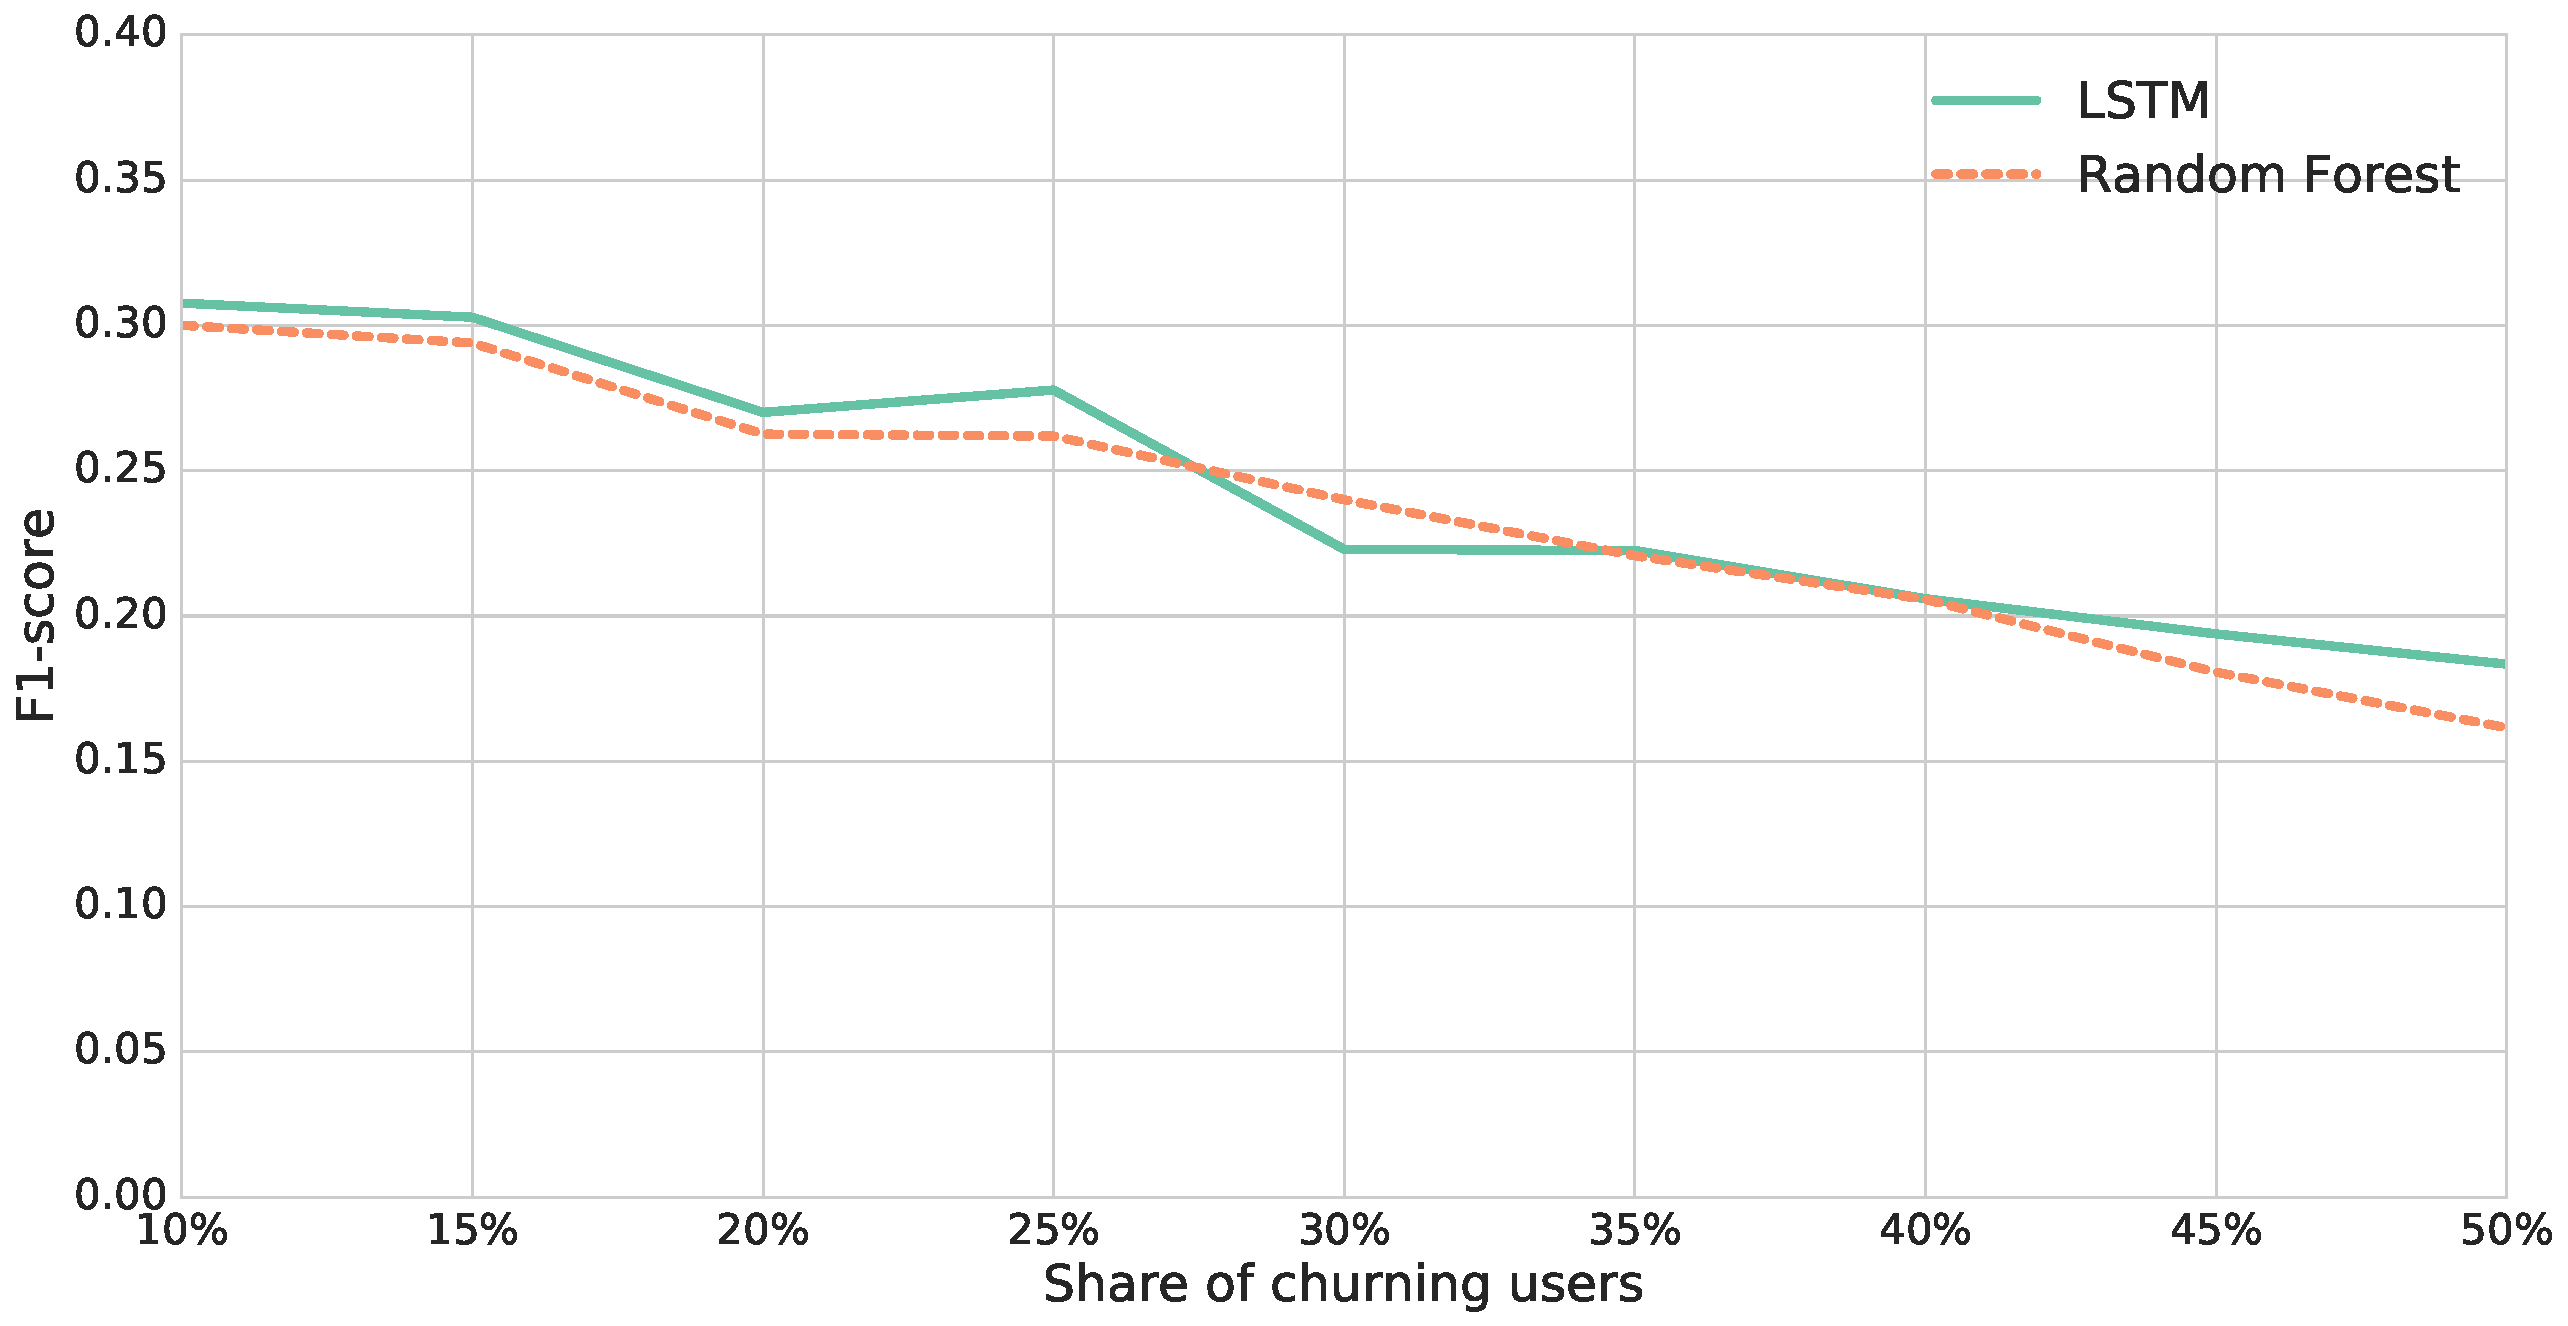
\includegraphics[width=1.0\textwidth,keepaspectratio]{figures/line_class_balance.pdf}
    \caption{F1-scores of the positive churning class for different shares of churning users}
    \label{fig:line_class_balance}
\end{figure}

\begin{figure}
    \centering
    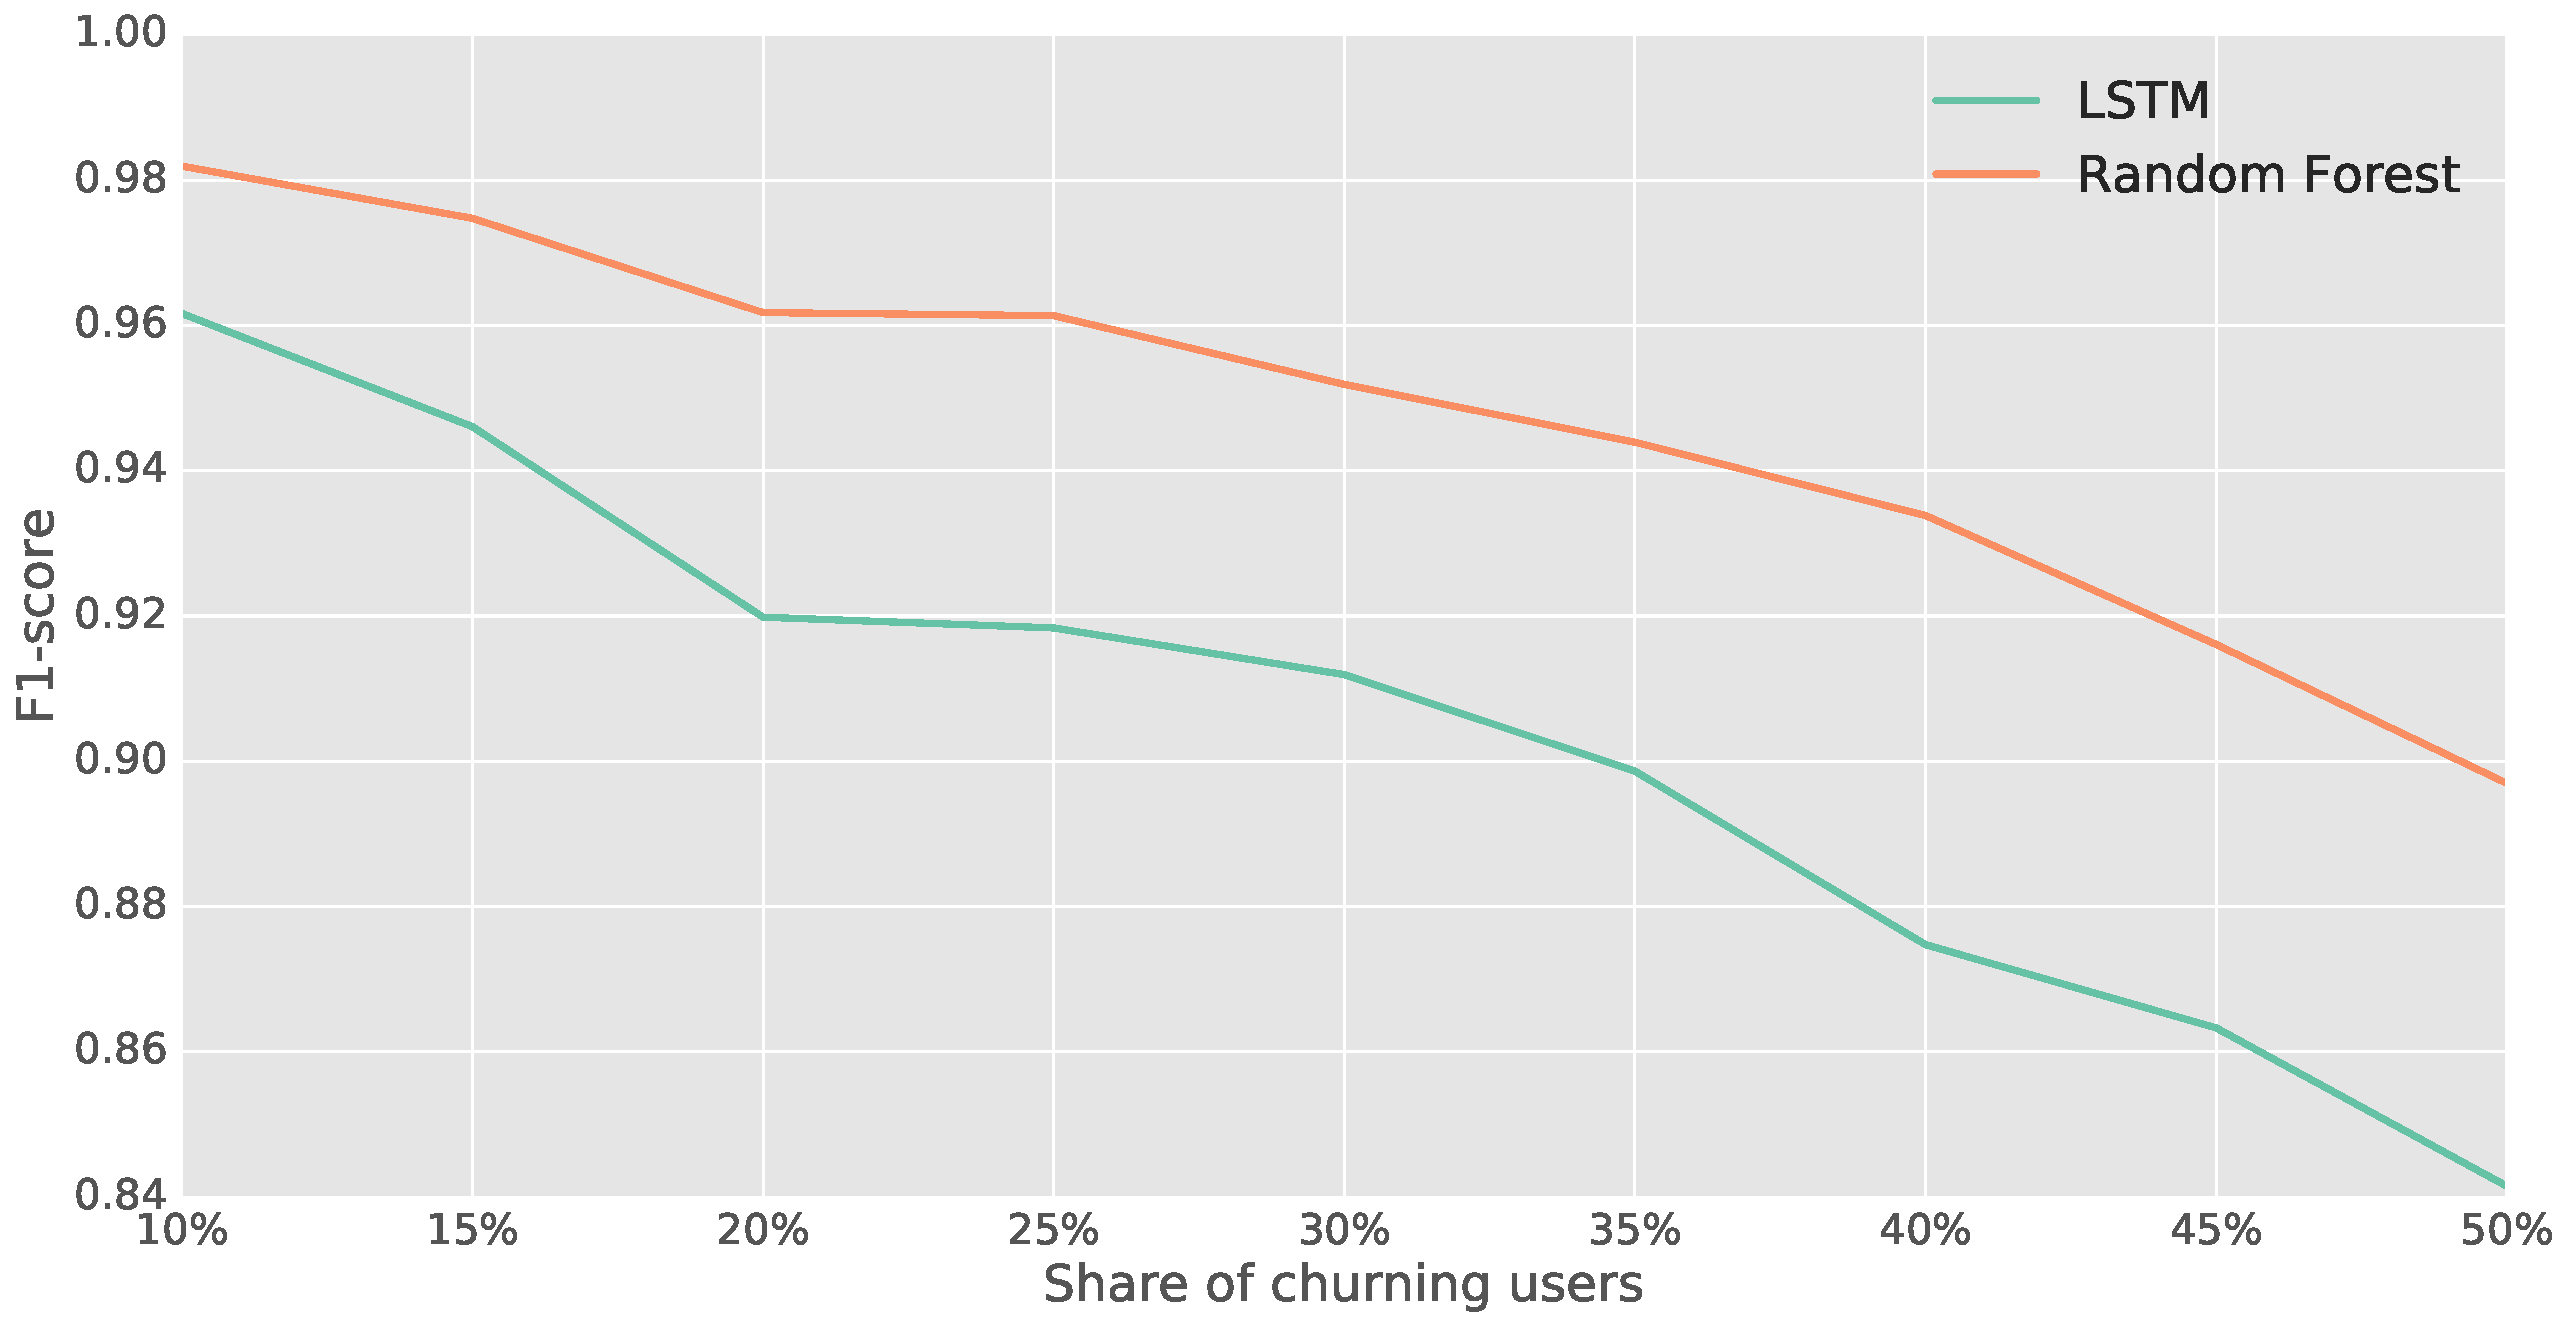
\includegraphics[width=1.0\textwidth,keepaspectratio]{figures/line_class_balance_retained.pdf}
    \caption{F1-scores of the negative retained class for different shares of churning users}
    \label{fig:line_class_balance_ret}
\end{figure}

The resulting F1-scores of this experiment for both the churning and retaining classes can be seen in \autoref{fig:line_class_balance} and \autoref{fig:line_class_balance_ret}, respectively. Interestingly the harmonic mean between precision and recall steadily reduces for both classes and models being experimented on. As can be seen in \autoref{tab:class_balance}, increasing the ratio of churning users by undersampling the majority class has an effect of increasing the recall metric, at the cost of a lower precision. If both metrics are equally weighted, the aggregated score suffer a significant decrease for the churning class as the gap between the churning and retaining users is reduced. 

This result is contrary to what is exposed by Burez and Van den Poel \citep{Burez2009}. In their study, there is a performance gain for using a less imbalanced dataset for training the predictor models,  however their main evaluation metric is ROC AUC, which could be mapped to our own results in \autoref{fig:roc_class_balance}. However the difference between different ratios in ROC AUC is minimal at best, mainly due to how heavily skewed the raw dataset is. 

\section{Experimenting with Dimensionality Reduction}

The dataset generated through our data pipeline is composed of 52 features related to the user behavior through time. It is intuitive to think that not all of these attributes will have the same importance when predicting if the user is going to churn or not, some of them may even be redundant in the presence of others. Having too many features may also lead to phenomenon known as "curse of dimensionality", where predictor models that learn through similarity of samples (implicitly or explicitly) may fail to achieve a good performance because examples are further apart from each other as more dimensions are used for representing the data \citep{domingos2012few}. 

Often the samples can be explained with some controlled loss of information by using a lower dimensional representation of the data. A common dimensionality reduction technique widely used for compression and visualization that strives to maximize the variance of the dataset is PCA. In this experiment, we attempt to find an optimal data format that maximizes the accuracy of our predictor models by pre-processing it through PCA while gradually increasing the number of principal components the data is reduced to, being the last tested value all 52 features of the original dataset with no compression. Logistic regression is once again removed from this experiment due to poor performance in the previous analysis.

\begin{figure}
    \centering
    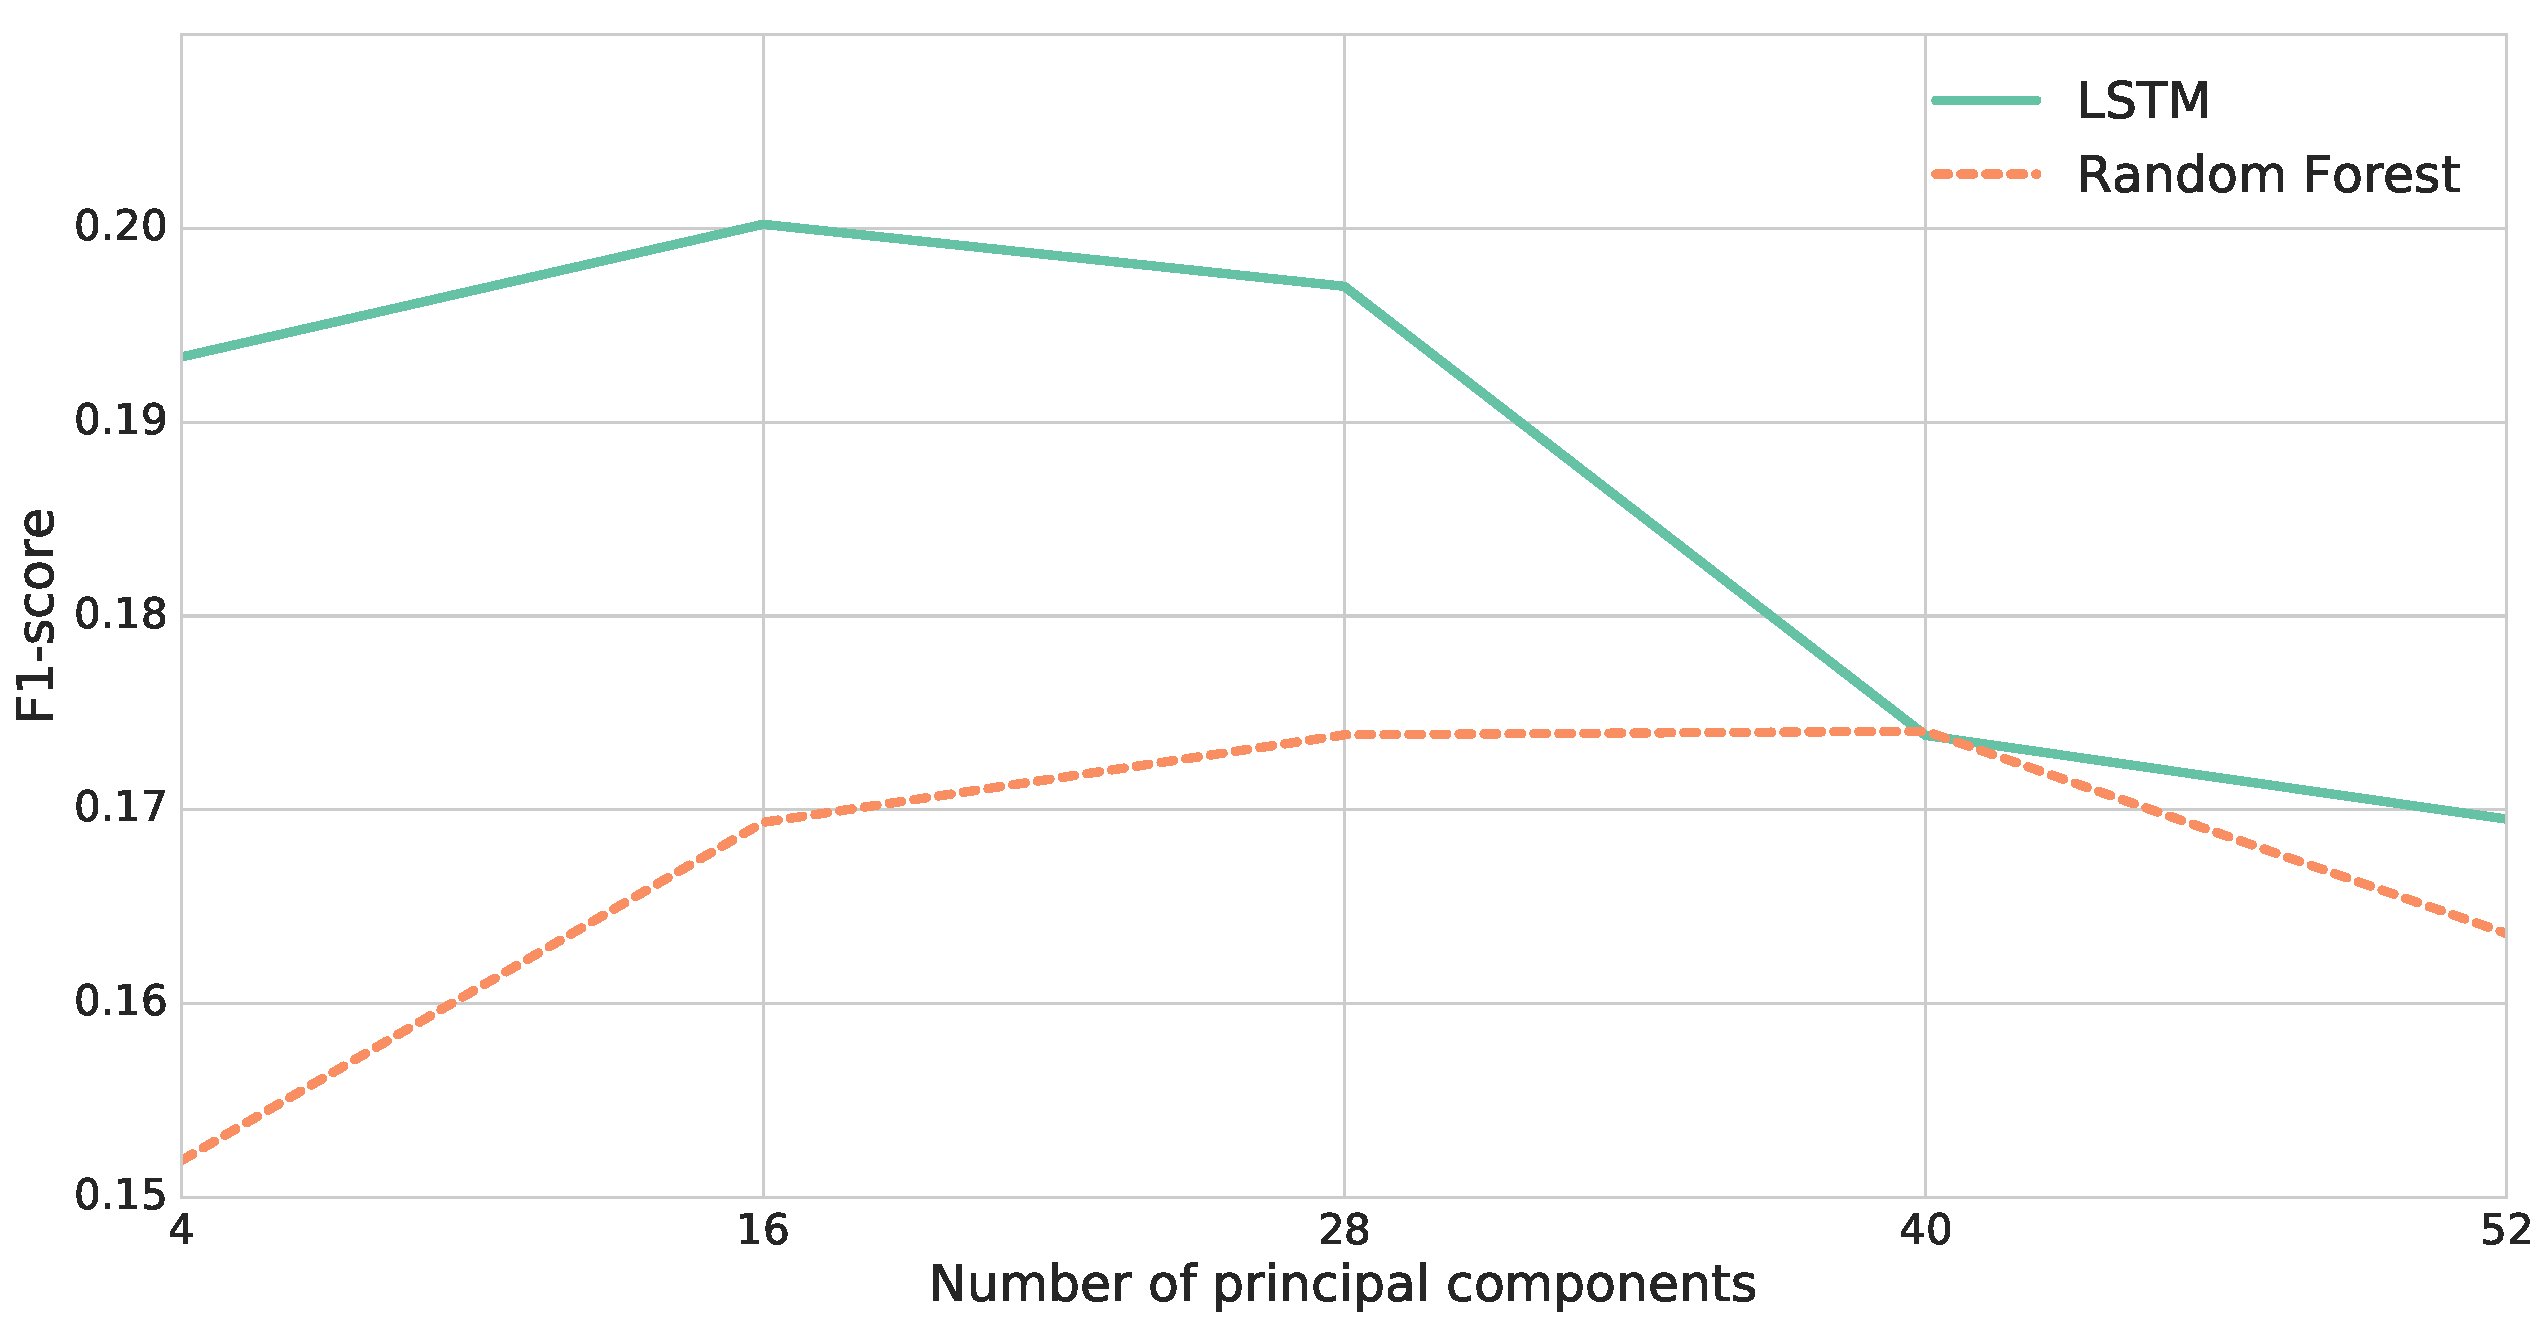
\includegraphics[width=1.0\textwidth,keepaspectratio]{figures/line_dim_reduction.pdf}
    \caption{F1-scores of the positive churning class for different number of principal components}
    \label{fig:line_dim_reduction}
\end{figure}

\begin{figure}
    \centering
    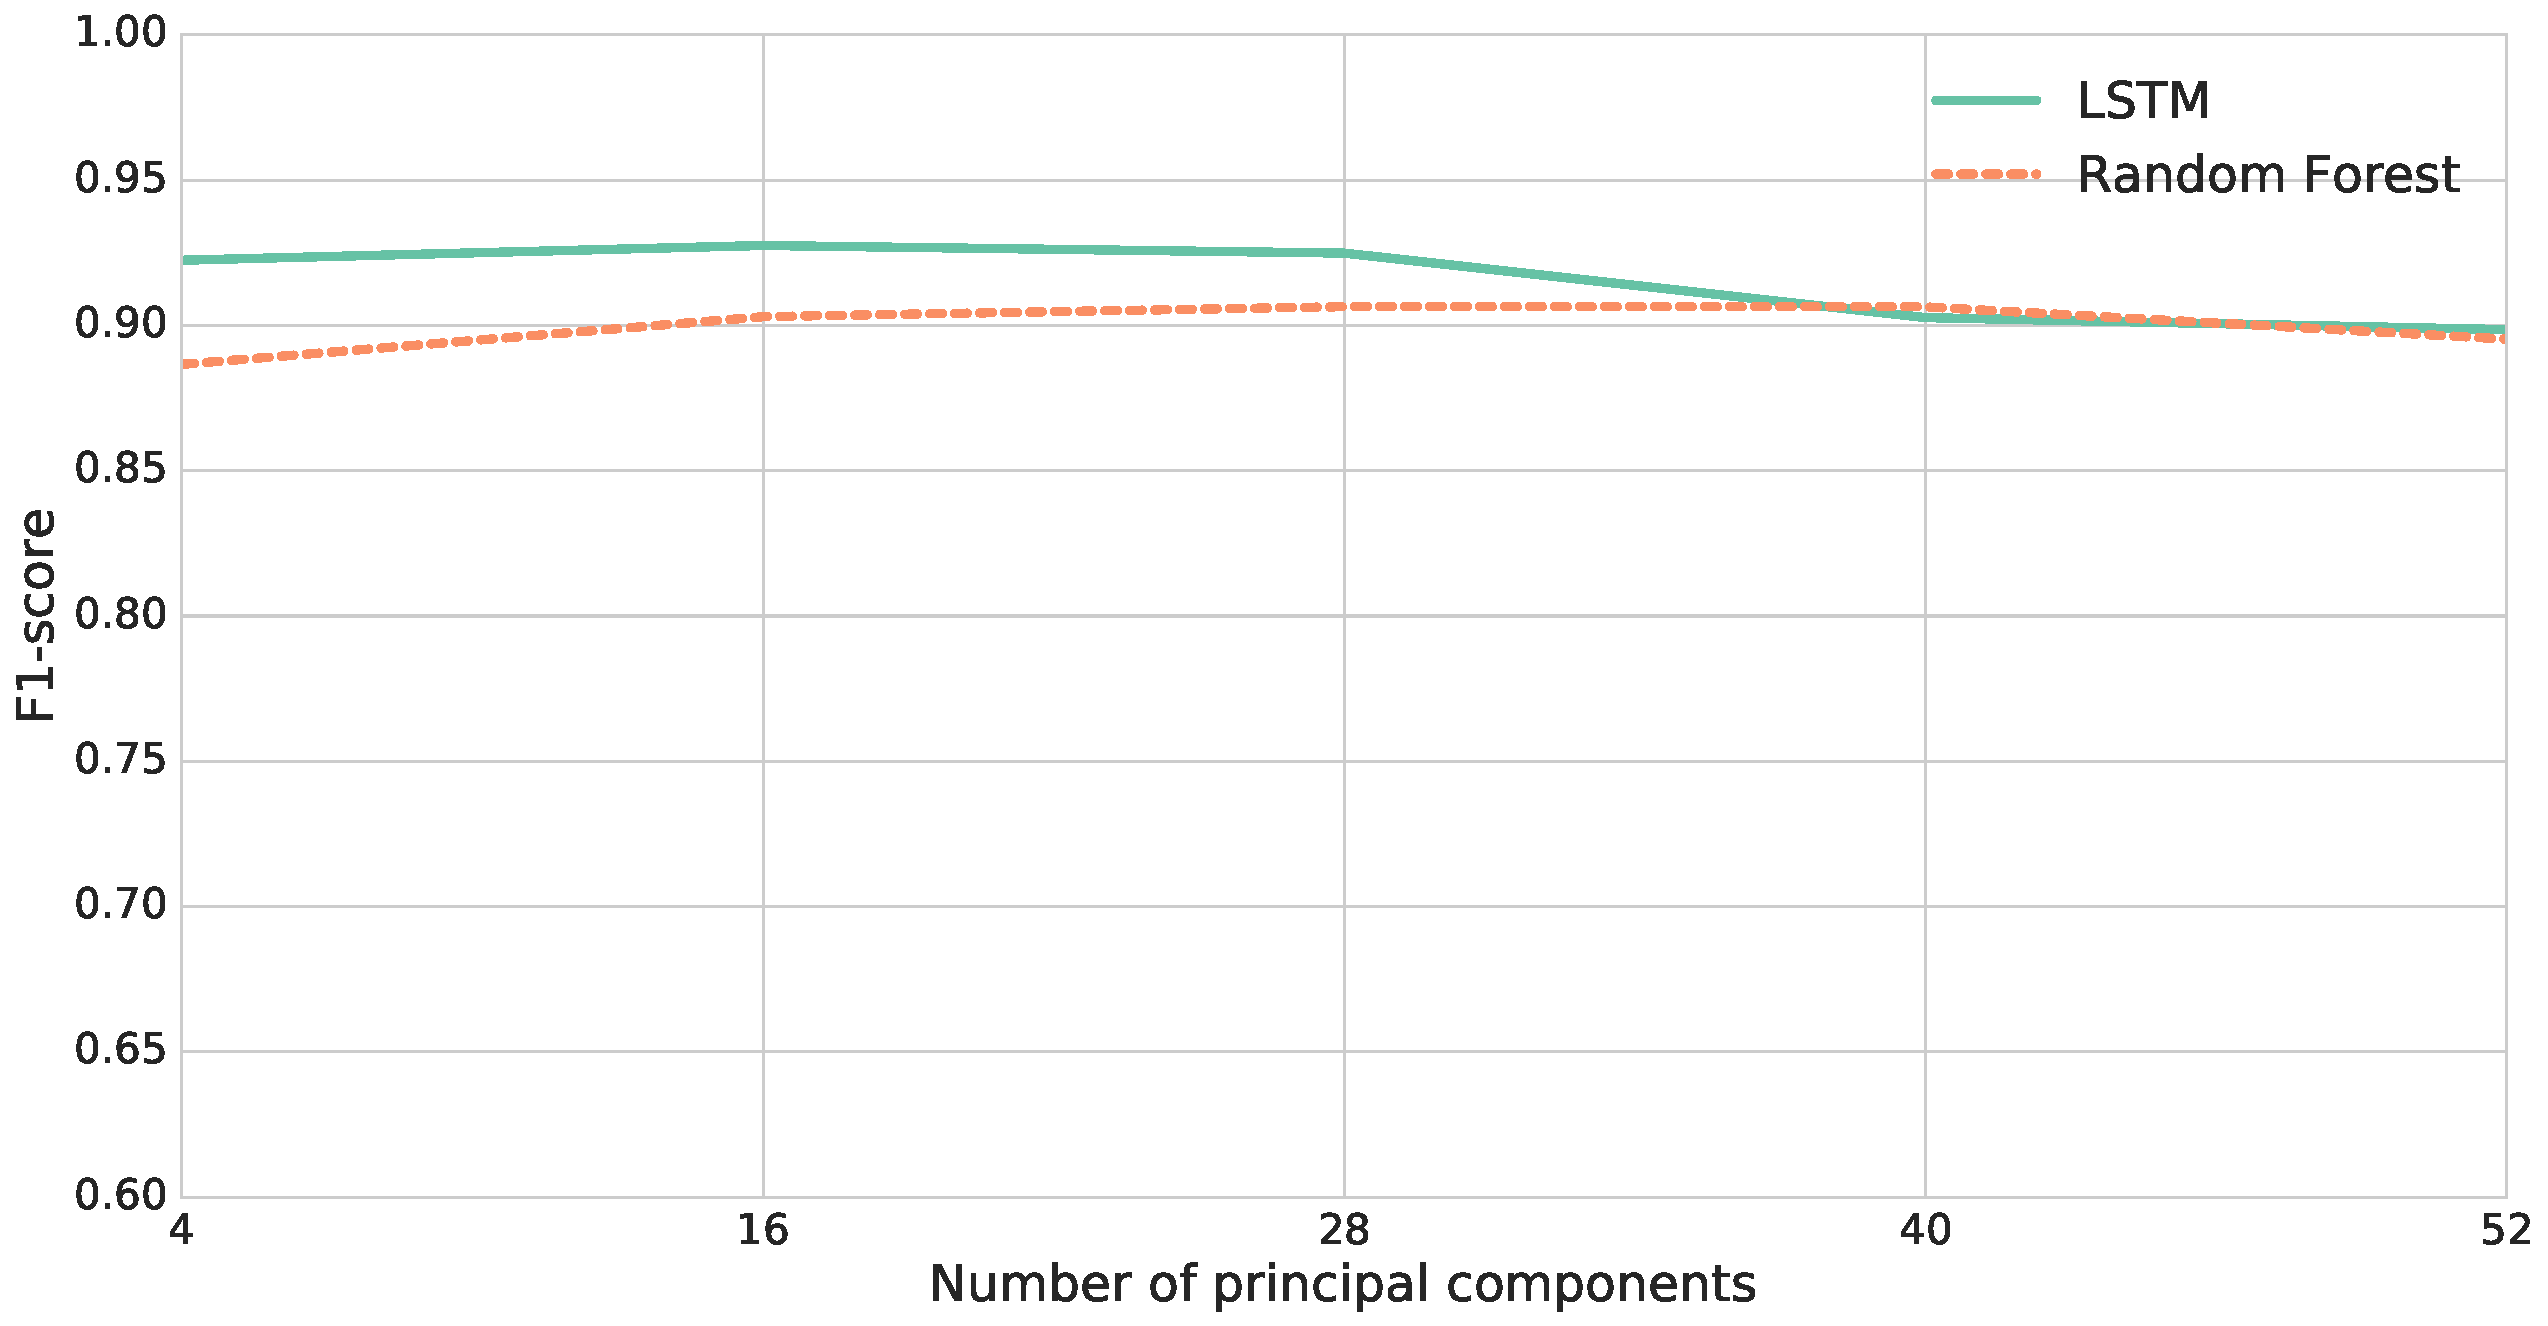
\includegraphics[width=1.0\textwidth,keepaspectratio]{figures/line_dim_reduction_retained.pdf}
    \caption{F1-scores of the negative retained class for different number of principal components}
    \label{fig:line_dim_reduction_ret}
\end{figure}

The results of this experiment can be seen in \autoref{fig:line_dim_reduction} and \autoref{fig:line_dim_reduction_ret}. Here it can be seen that by selecting 16 principal components after reducing the data through PCA achieves highest F1-scores for both retaining and churning classes in the LSTM model, however the increase is not large, a difference of $0.04$ of the metric between the highest and the uncompressed data for the churned class, and even less when evaluating the retaining users.

Random forests exhibit a similar behavior, but peaking at 40 principal components instead. The gain however is marginal: around $0.01$ of F1-score increase when compared to the full dataset, for both retaining and churning users. Extensive metrics can be seen in the precision-recall curves, ROC curves and metrics table at \autoref{fig:prc_dim_reduction}, \autoref{fig:roc_dim_reduction} and \autoref{tab:dim_reduction}, respectively.

\chapter{Conclusions and Future Work}

* Predicting when the user is churning (Regression LSTM vs. Survival Analysis)

* Ensemble methods using classifiers that can strongly predict the positive and negative classes

\bibliography{references}

\appendix

\chapter{Additional Results}
\label{chap:add_results}

\section{Precision-recall curves}

\begin{figure}
    \centering
    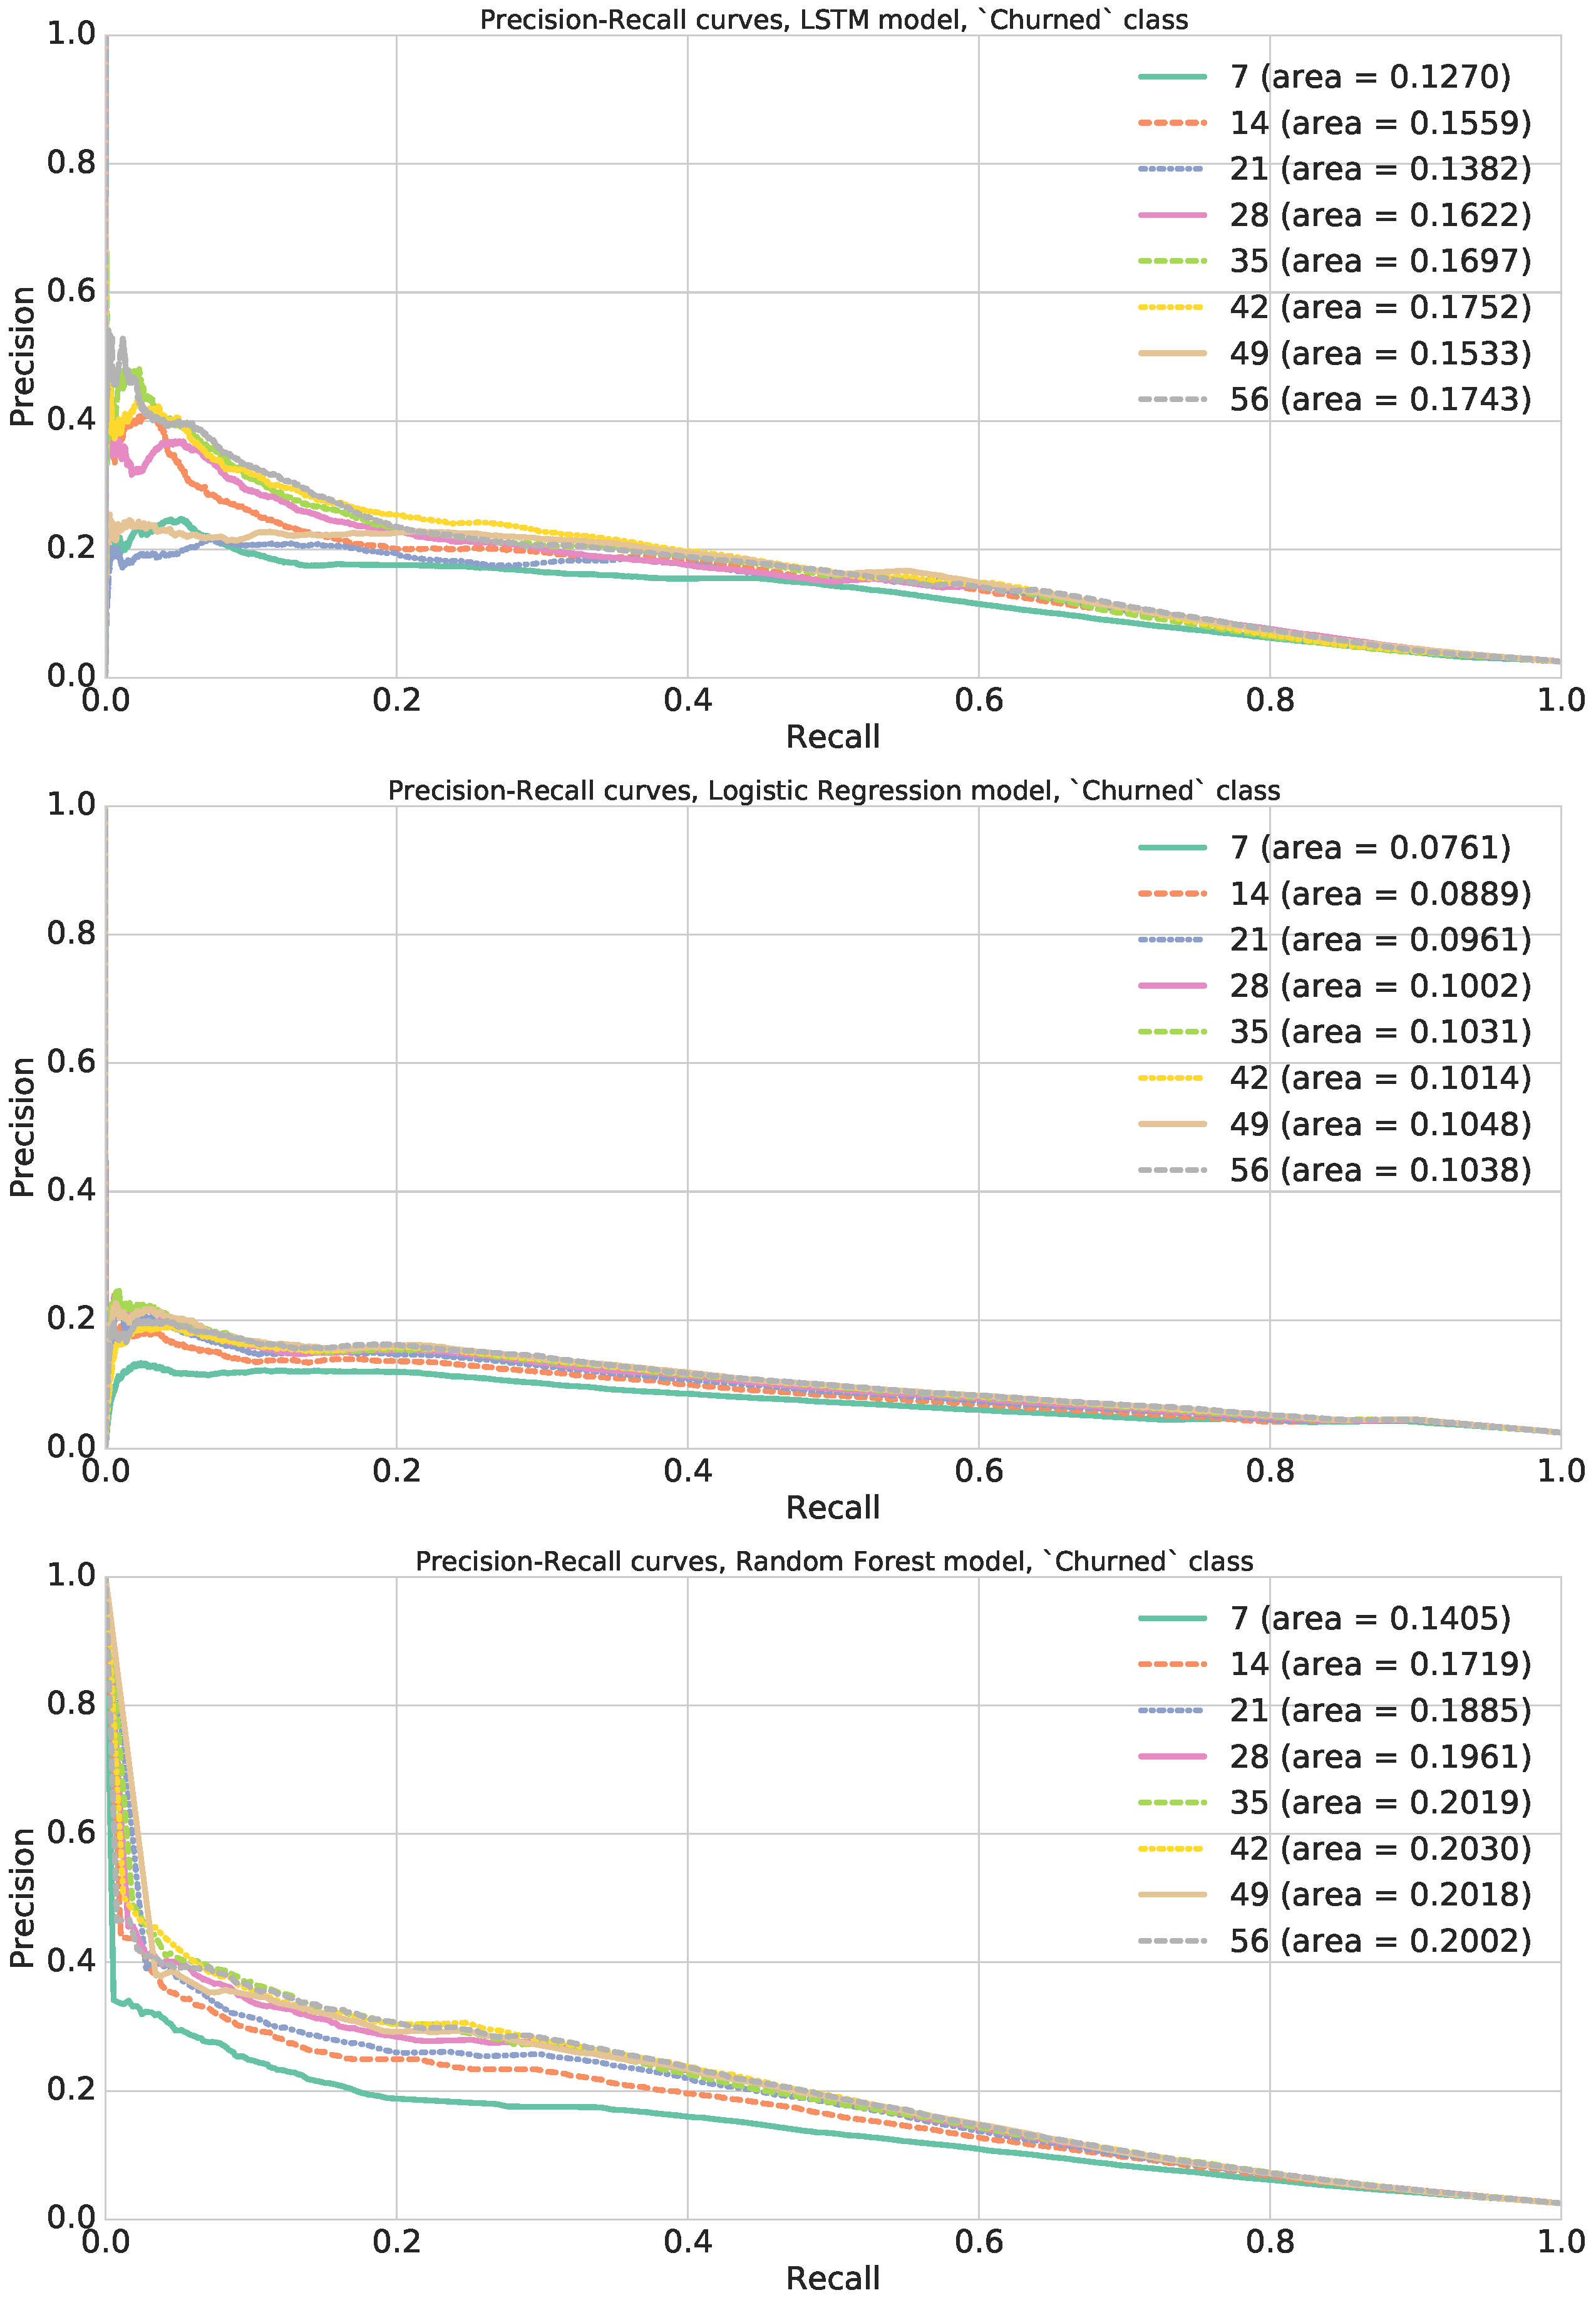
\includegraphics[width=1.0\textwidth,keepaspectratio]{figures/prc_obs_window.pdf}
    \caption{Precision-recall curves of the churned class for the observation window experiment.}
    \label{fig:prc_obs_window}
\end{figure}

\begin{figure}
    \centering
    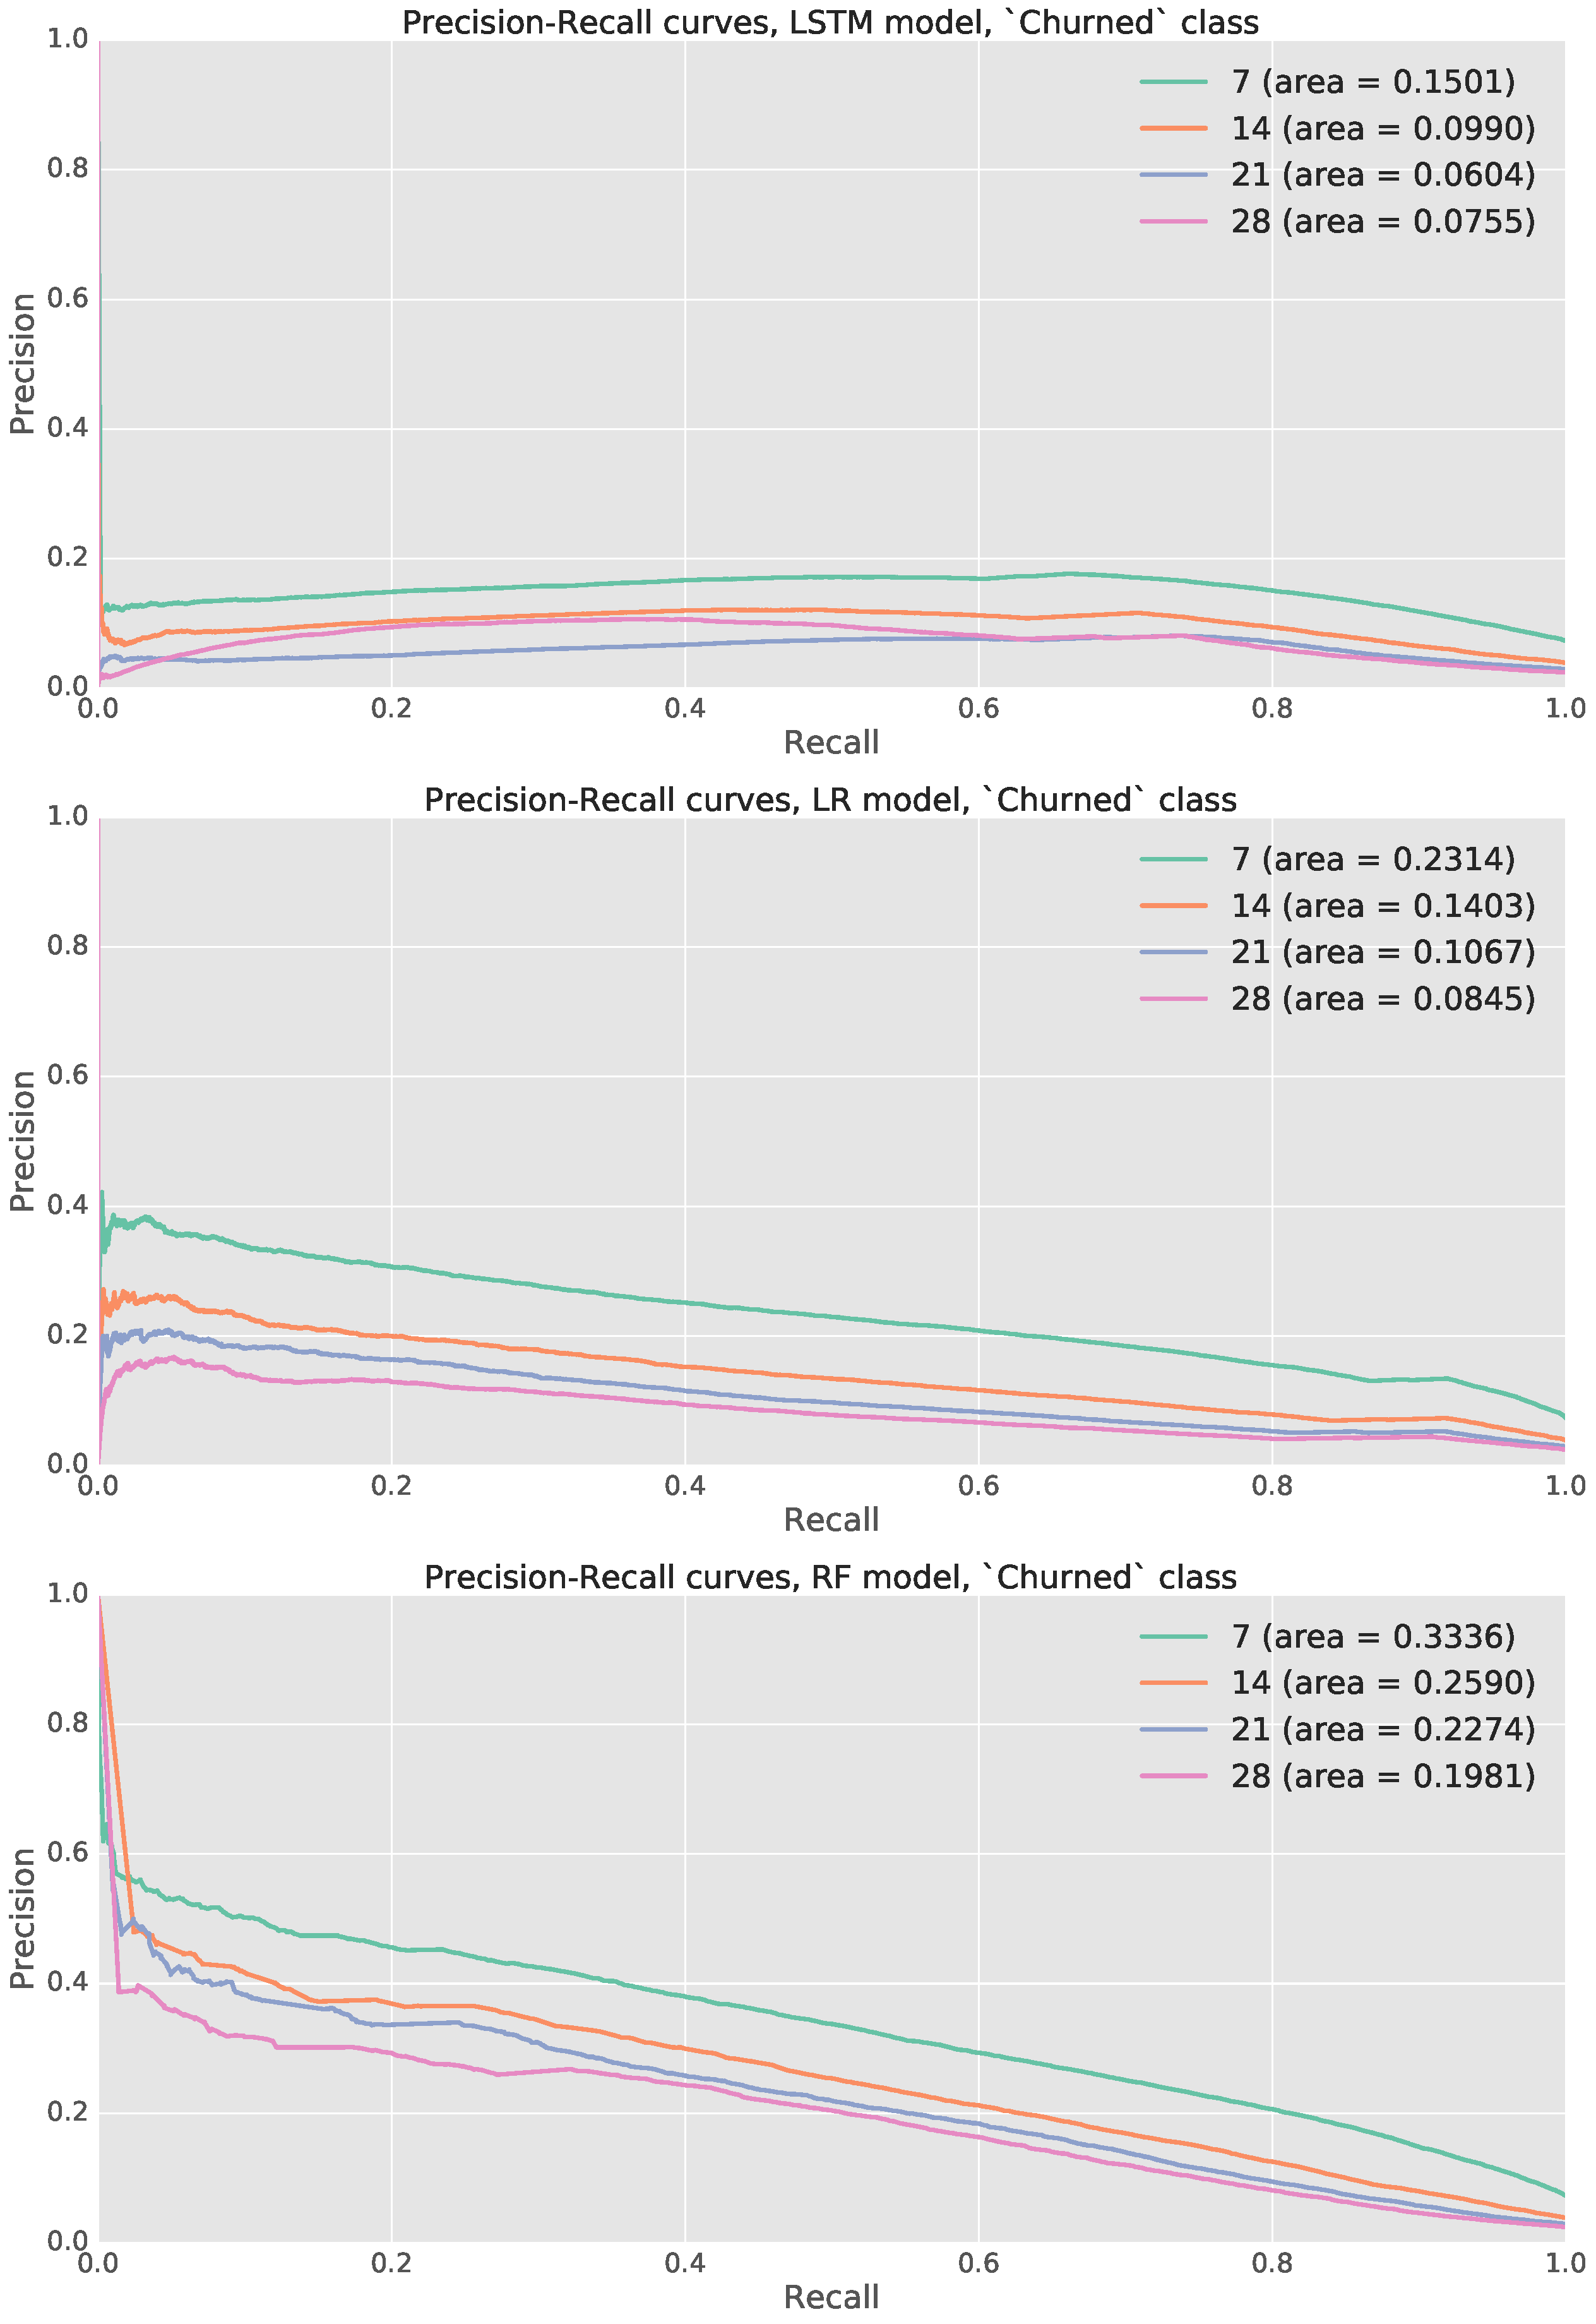
\includegraphics[width=1.0\textwidth,keepaspectratio]{figures/prc_pred_window.pdf}
    \caption{Precision-recall curves of the churned class for the prediction window experiment.}
    \label{fig:prc_pred_window}
\end{figure}

\begin{figure}
    \centering
    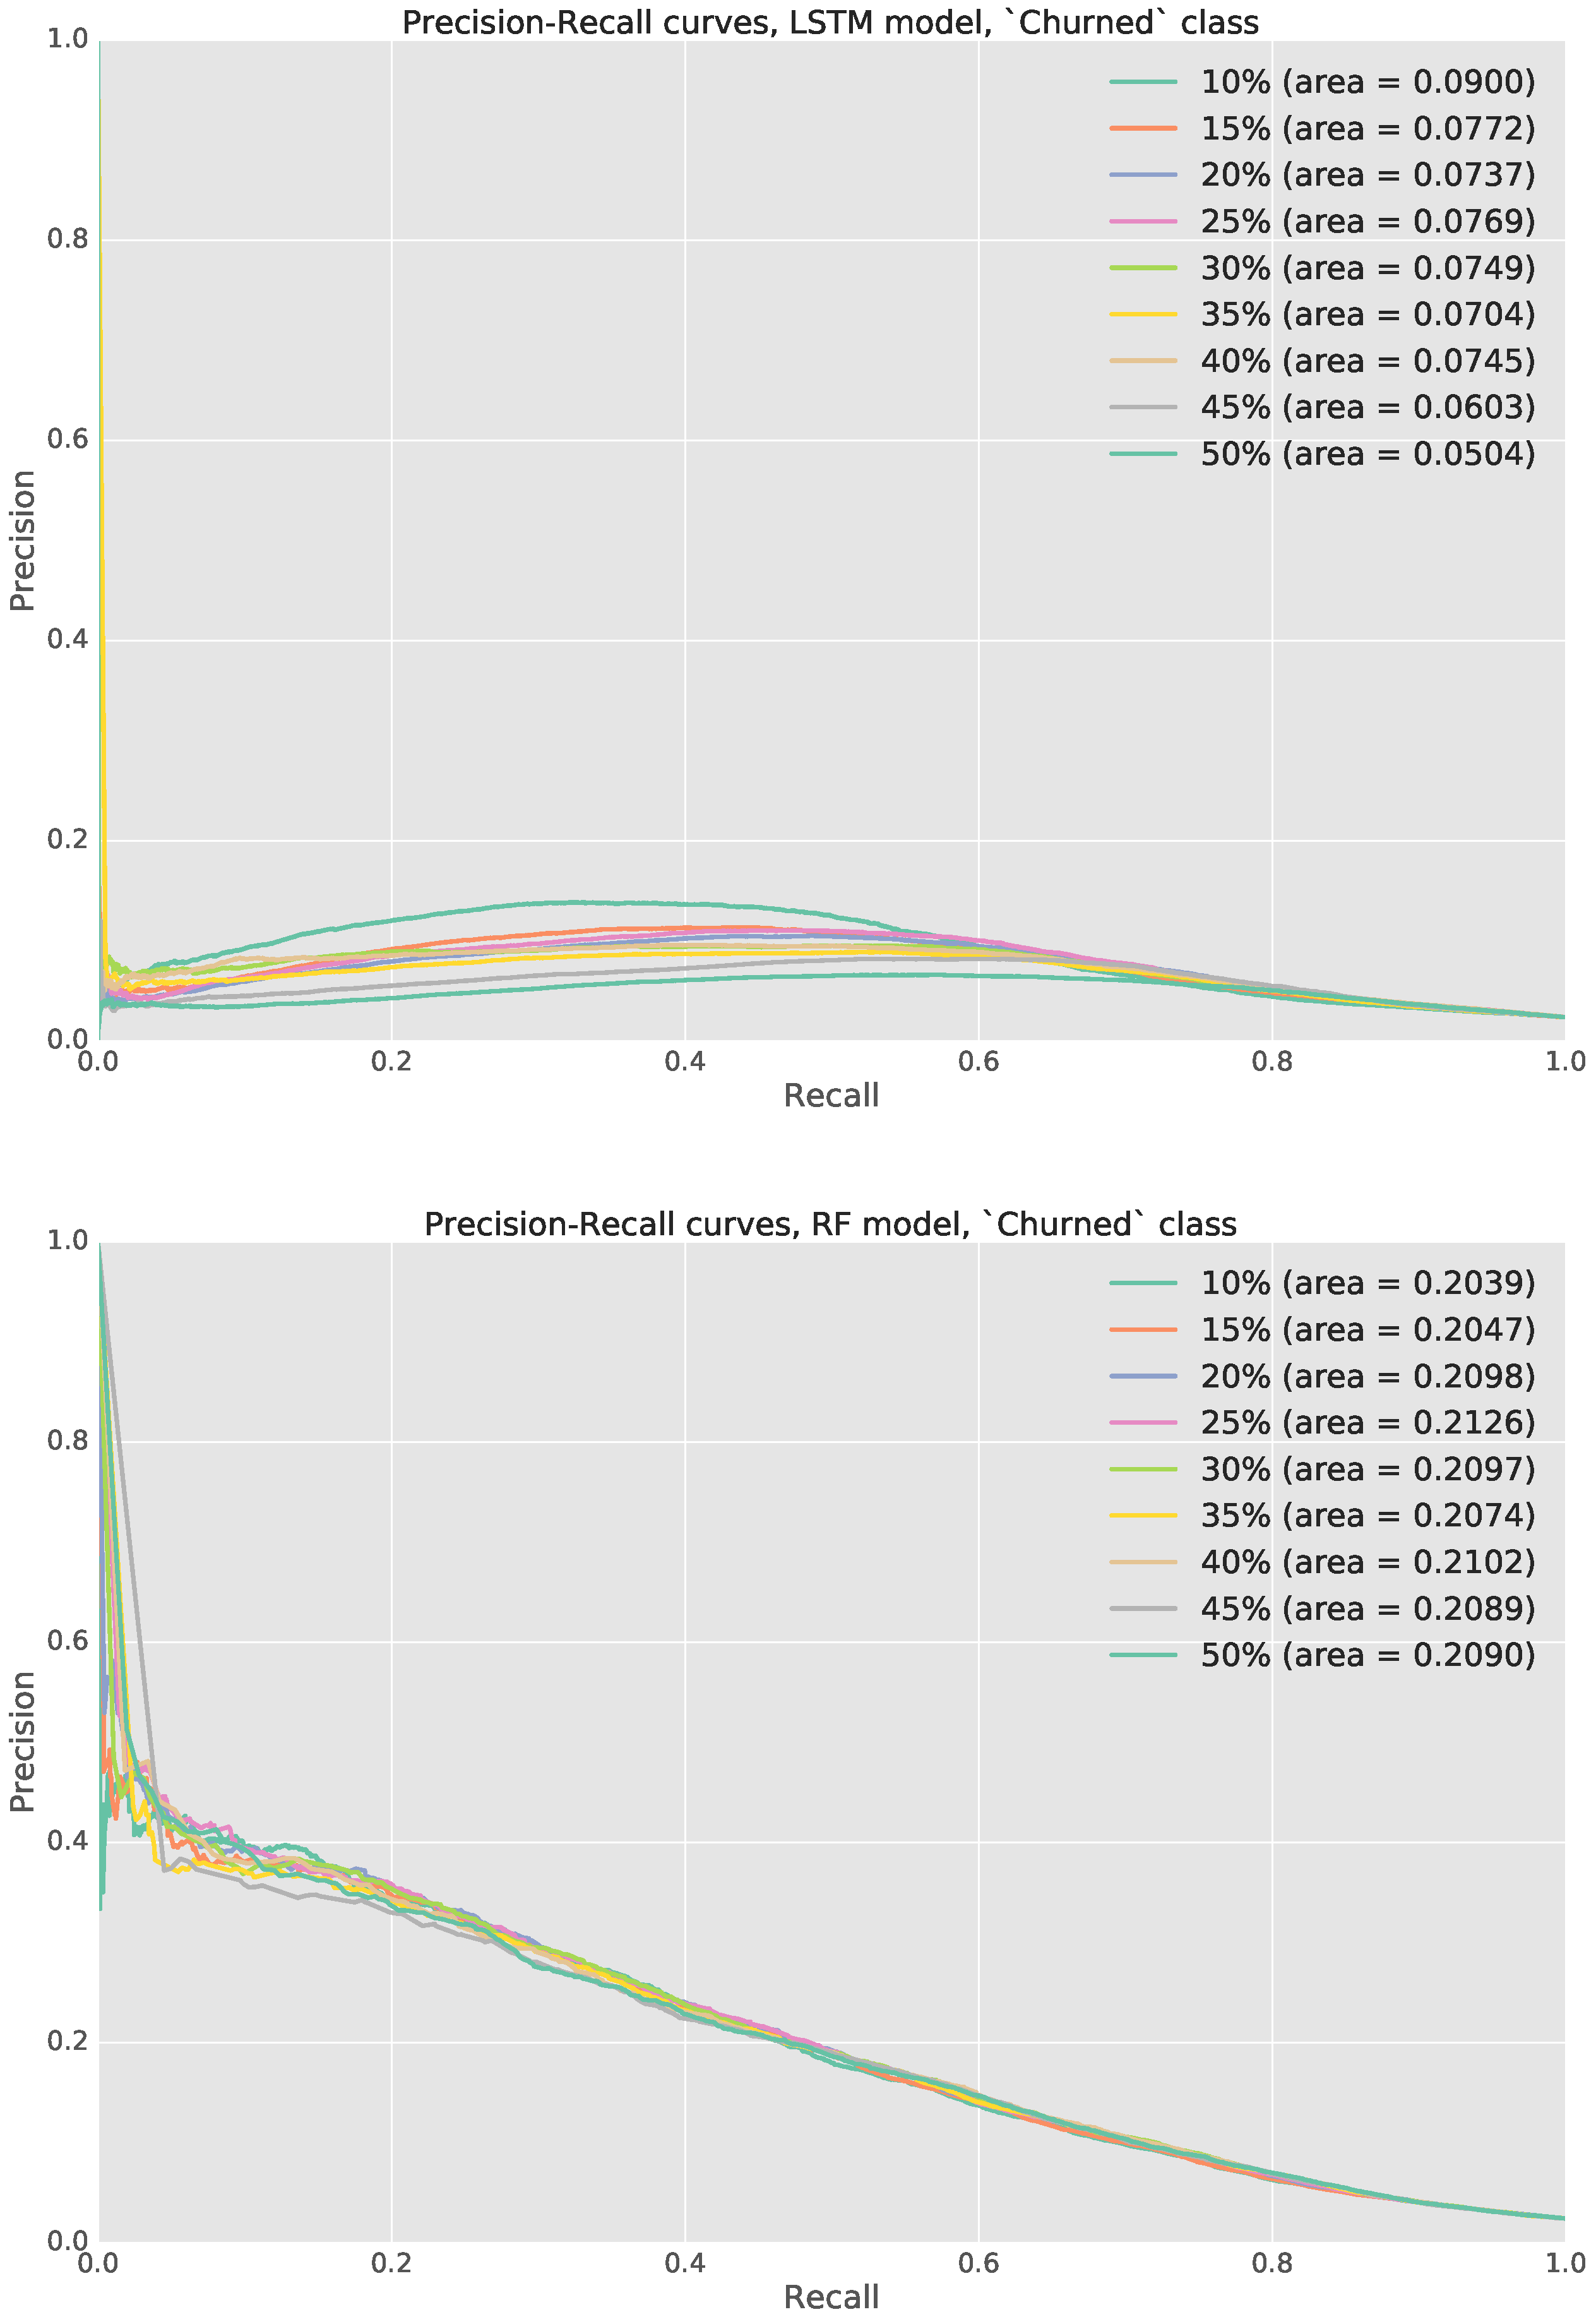
\includegraphics[width=1.0\textwidth,keepaspectratio]{figures/prc_class_balance.pdf}
    \caption{Precision-recall curves of the churned class for the class balance experiment.}
    \label{fig:prc_class_balance}
\end{figure}

\begin{figure}
    \centering
    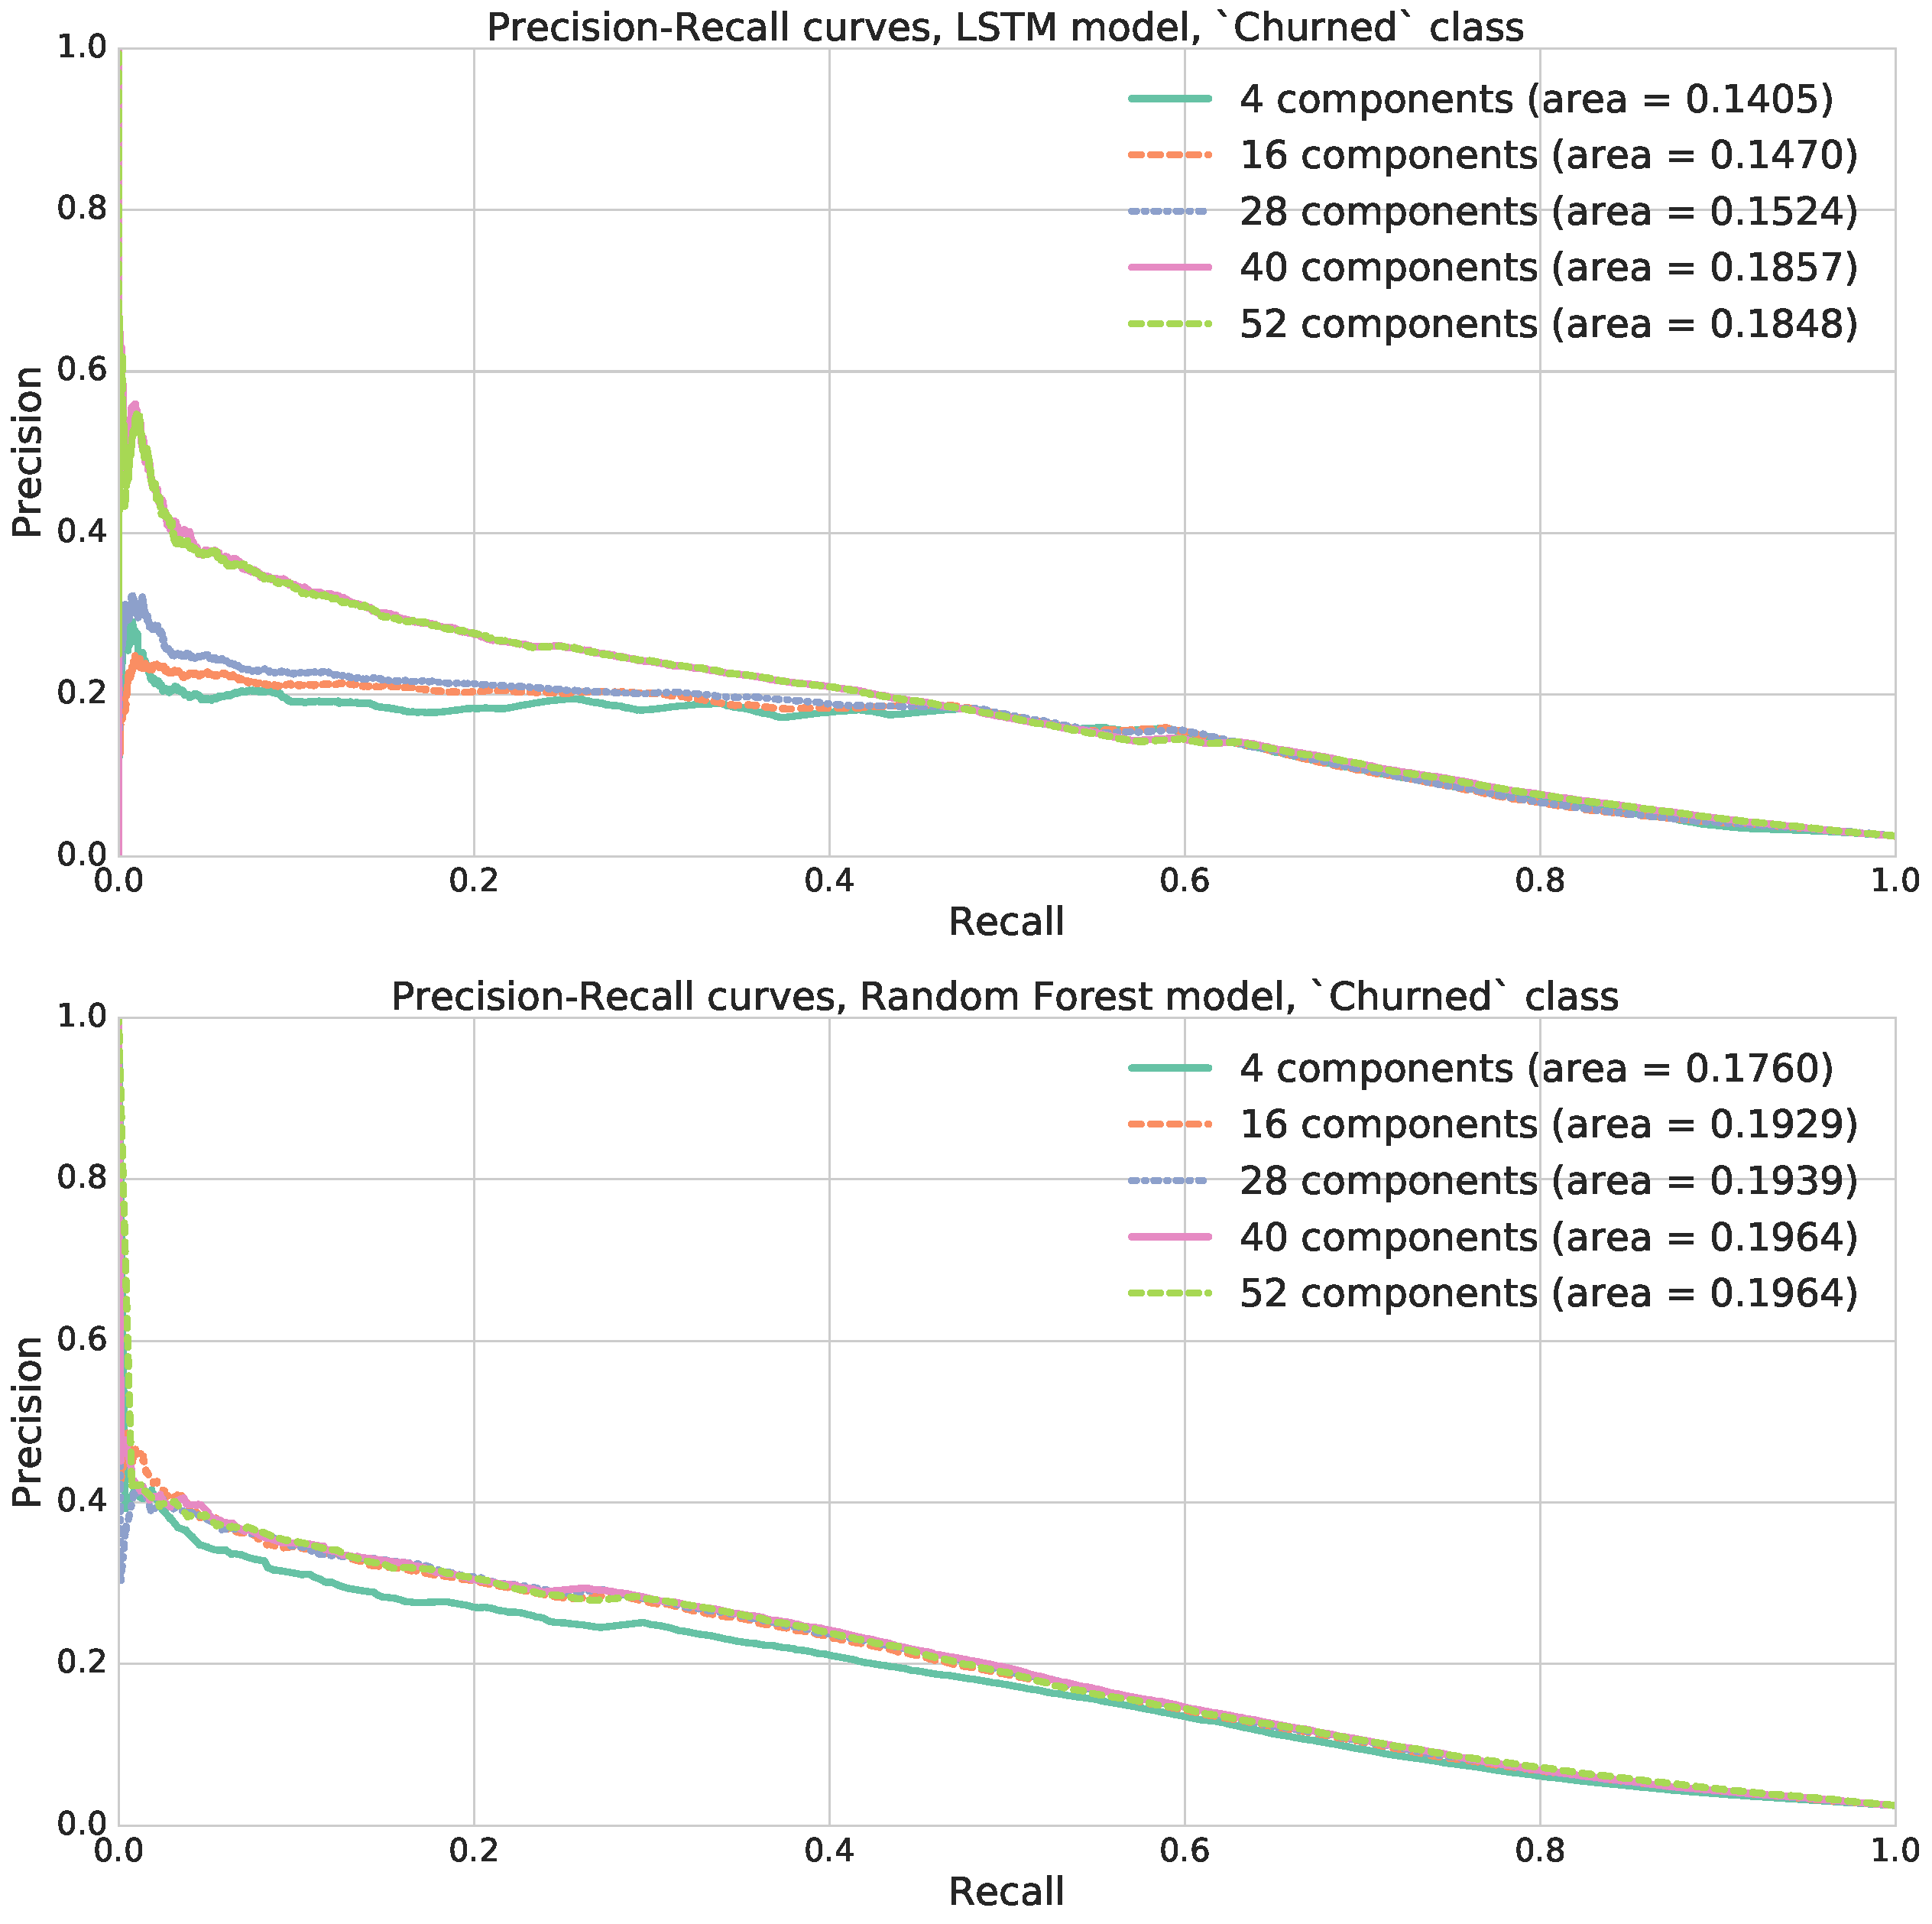
\includegraphics[width=1.0\textwidth,keepaspectratio]{figures/prc_dim_reduction.pdf}
    \caption{Precision-recall curves of the churned class for the dimensionality reduction experiment.}
    \label{fig:prc_dim_reduction}
\end{figure}

\section{ROC curves}

\begin{figure}
    \centering
    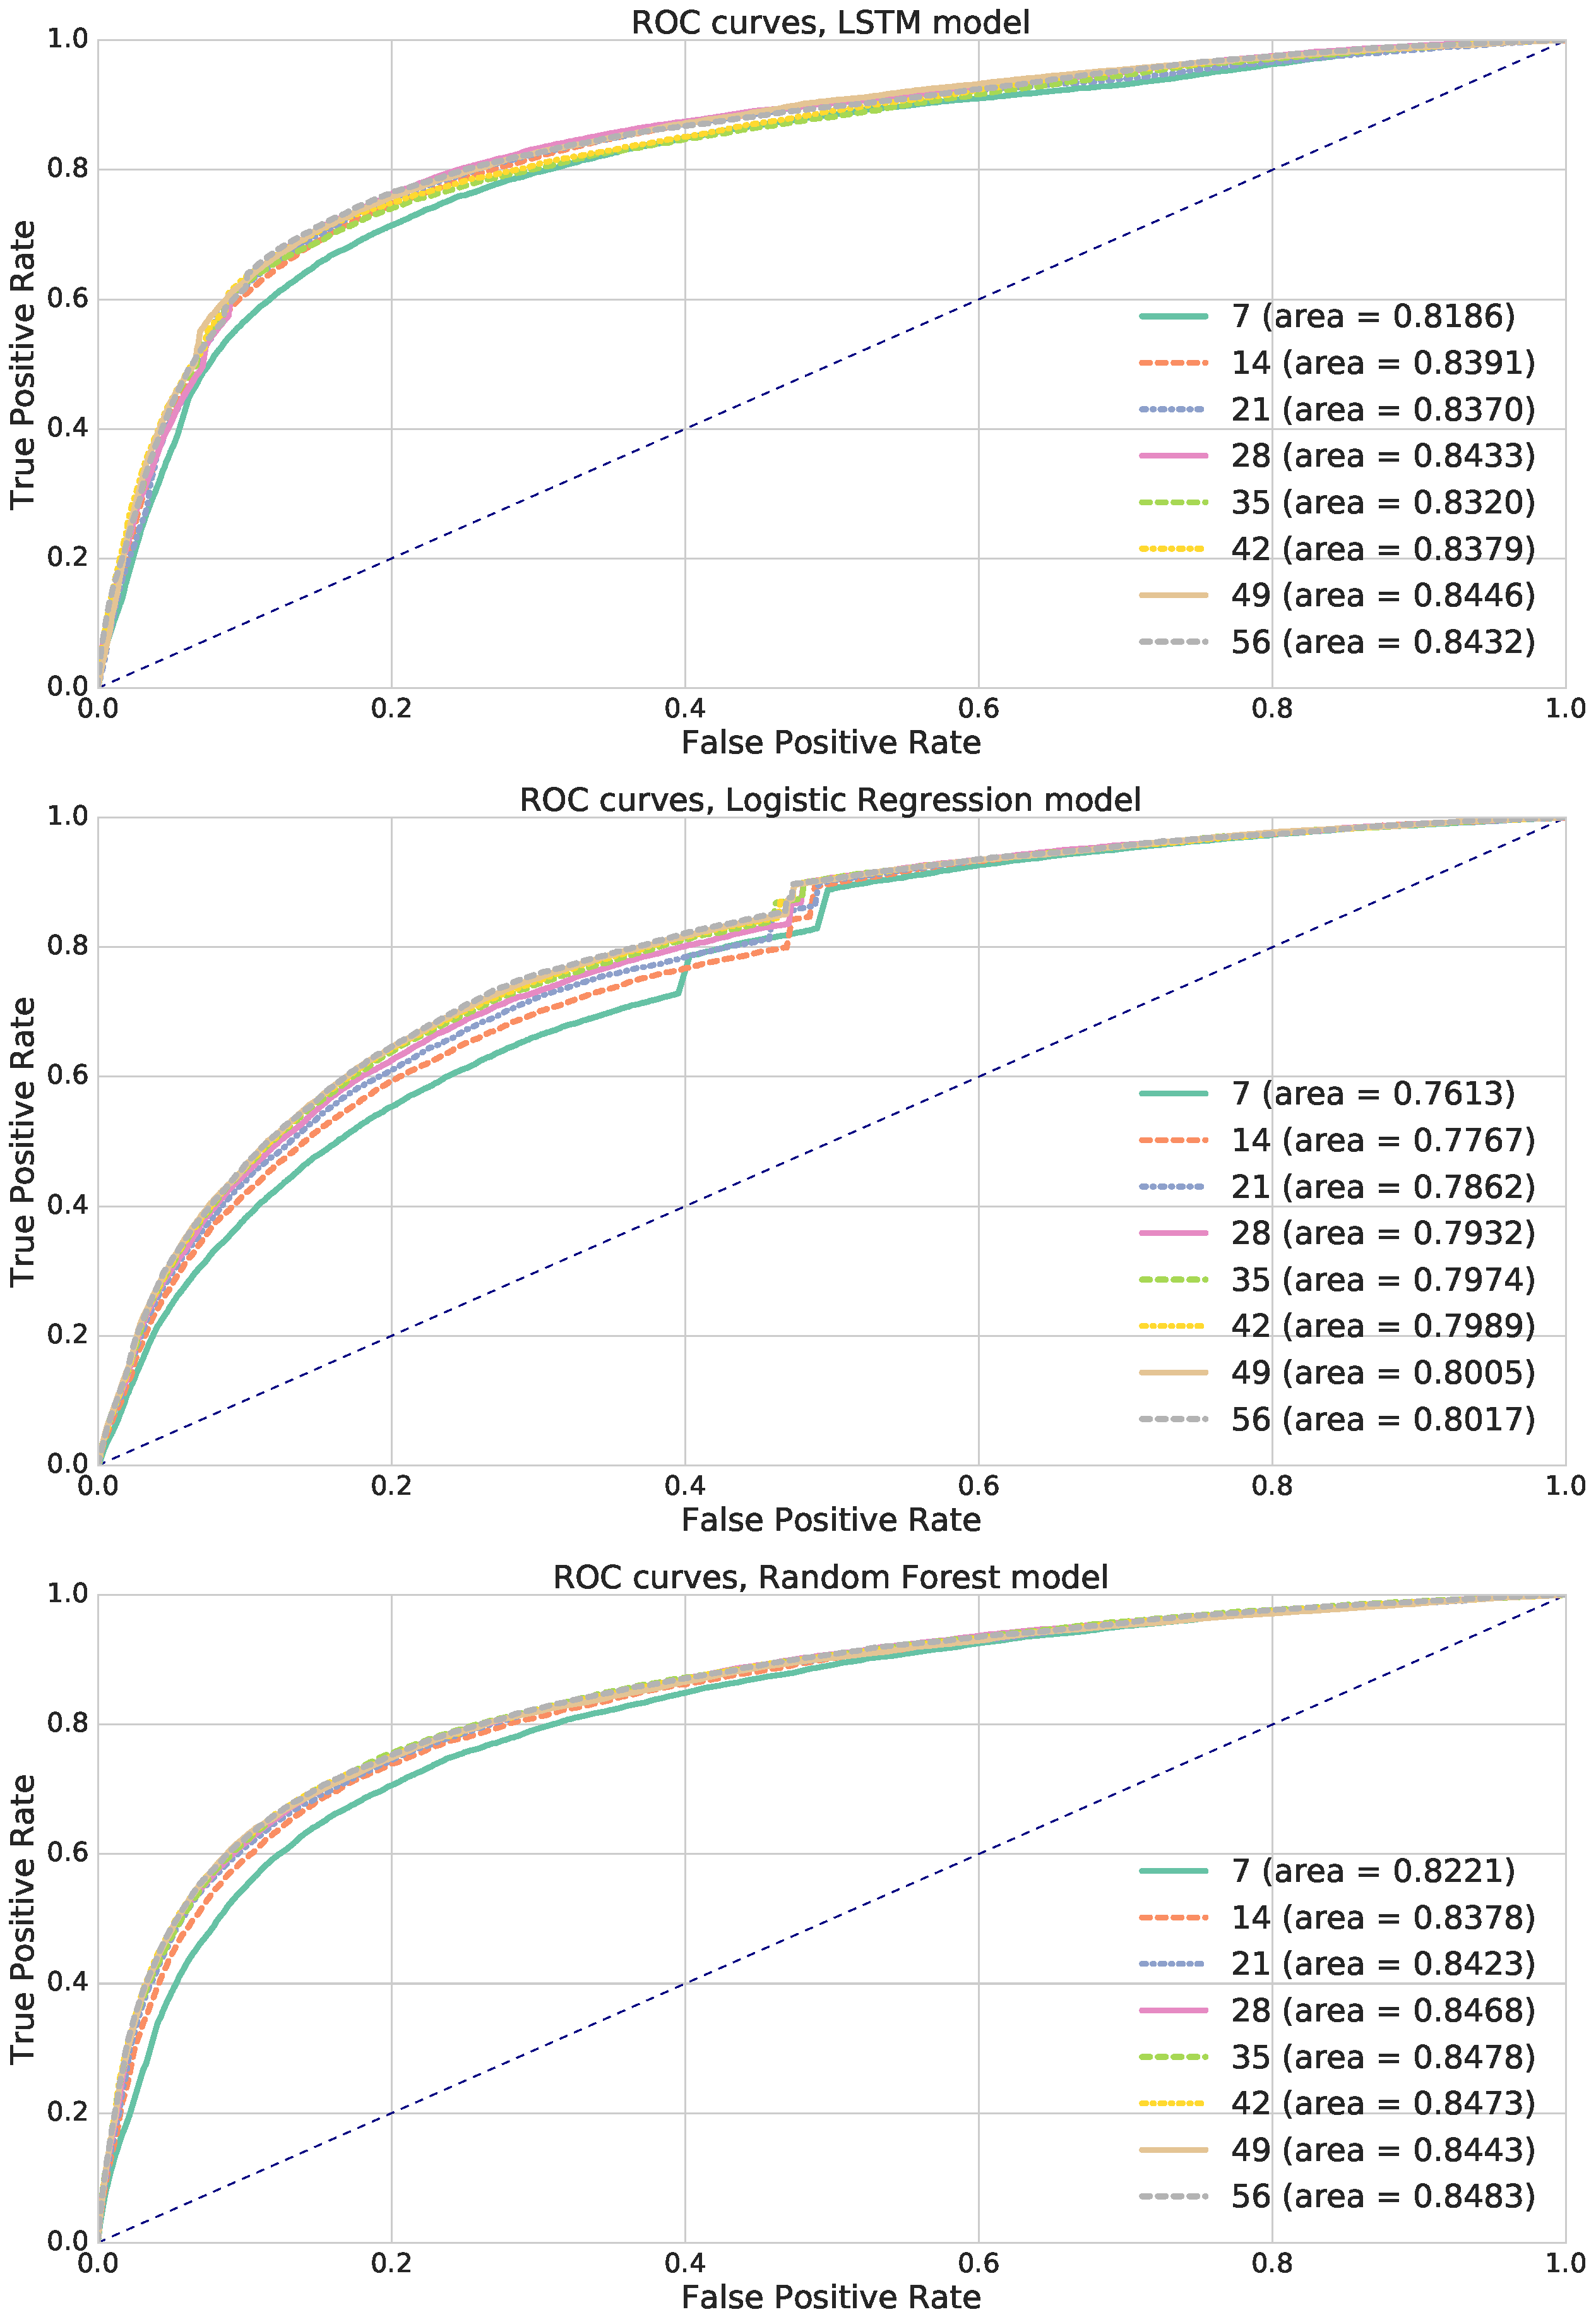
\includegraphics[width=1.0\textwidth,keepaspectratio]{figures/roc_obs_window.pdf}
    \caption{ROC curves for the observation window experiment}
    \label{fig:roc_obs_window}
\end{figure}

\begin{figure}
    \centering
    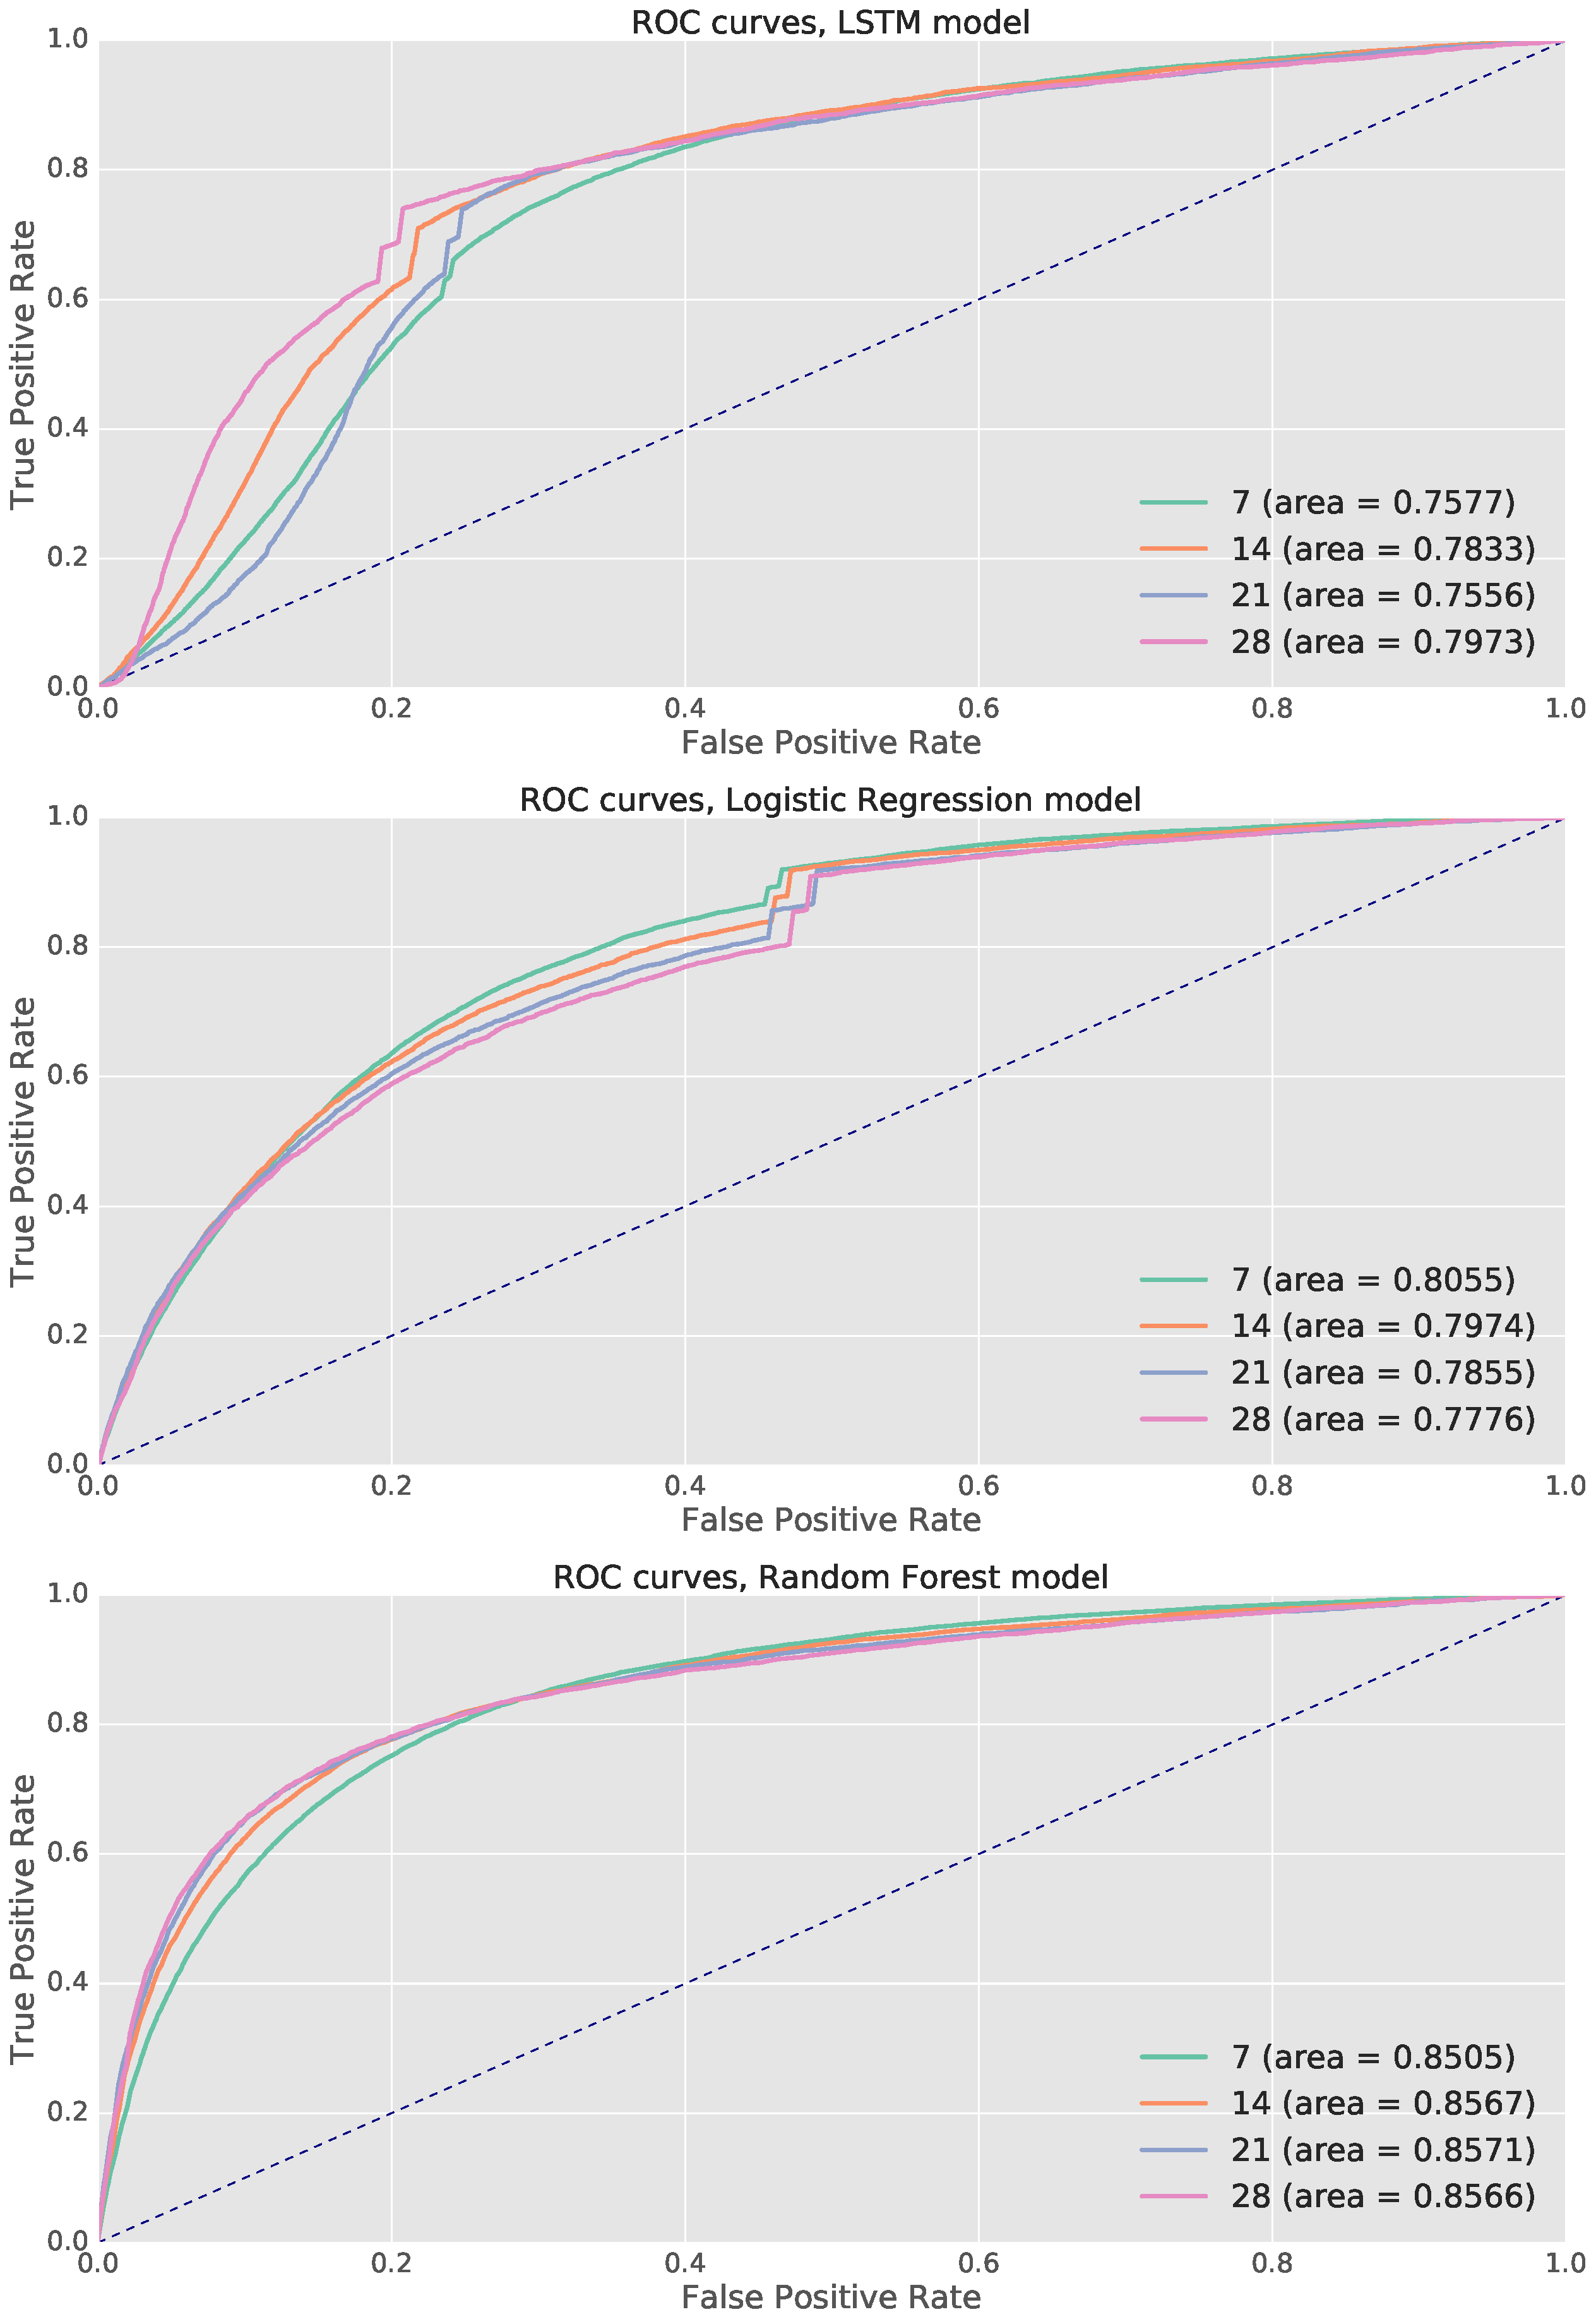
\includegraphics[width=1.0\textwidth,keepaspectratio]{figures/roc_pred_window.pdf}
    \caption{ROC curves for the prediction window experiment}
    \label{fig:roc_pred_window}
\end{figure}

\begin{figure}
    \centering
    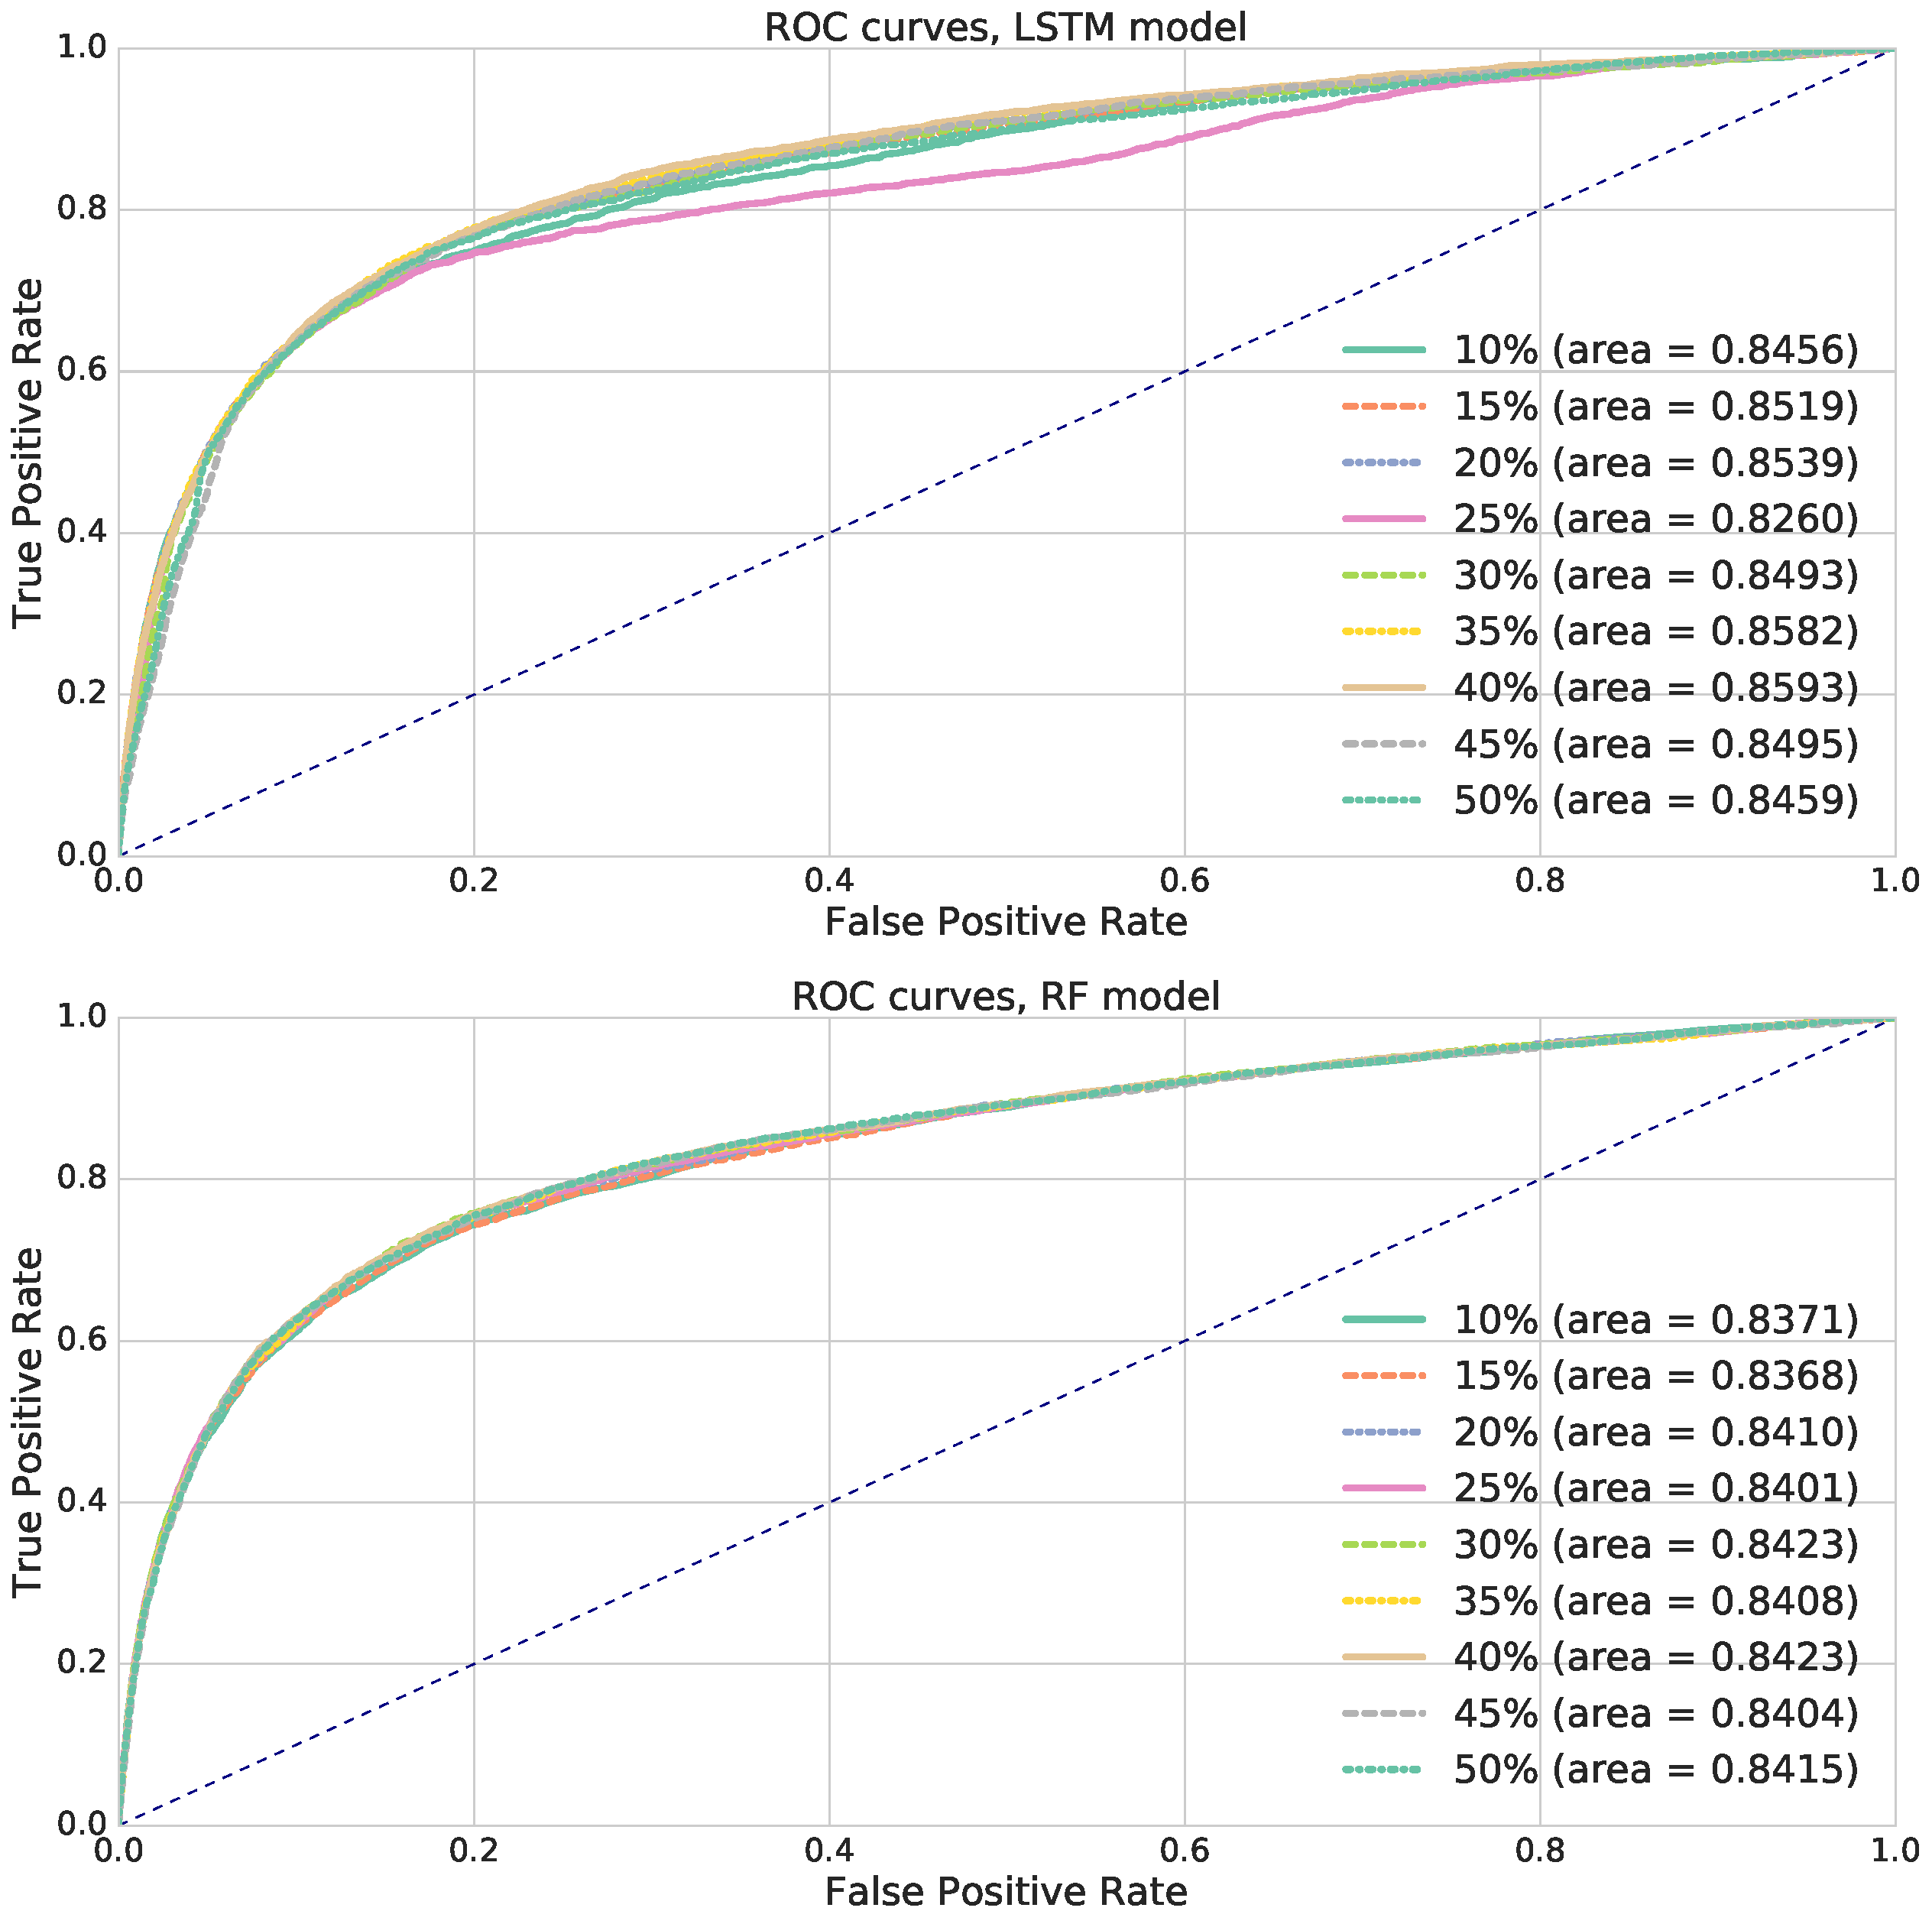
\includegraphics[width=1.0\textwidth,keepaspectratio]{figures/roc_class_balance.pdf}
    \caption{ROC curves for the class balance experiment}
    \label{fig:roc_class_balance}
\end{figure}

\begin{figure}
    \centering
    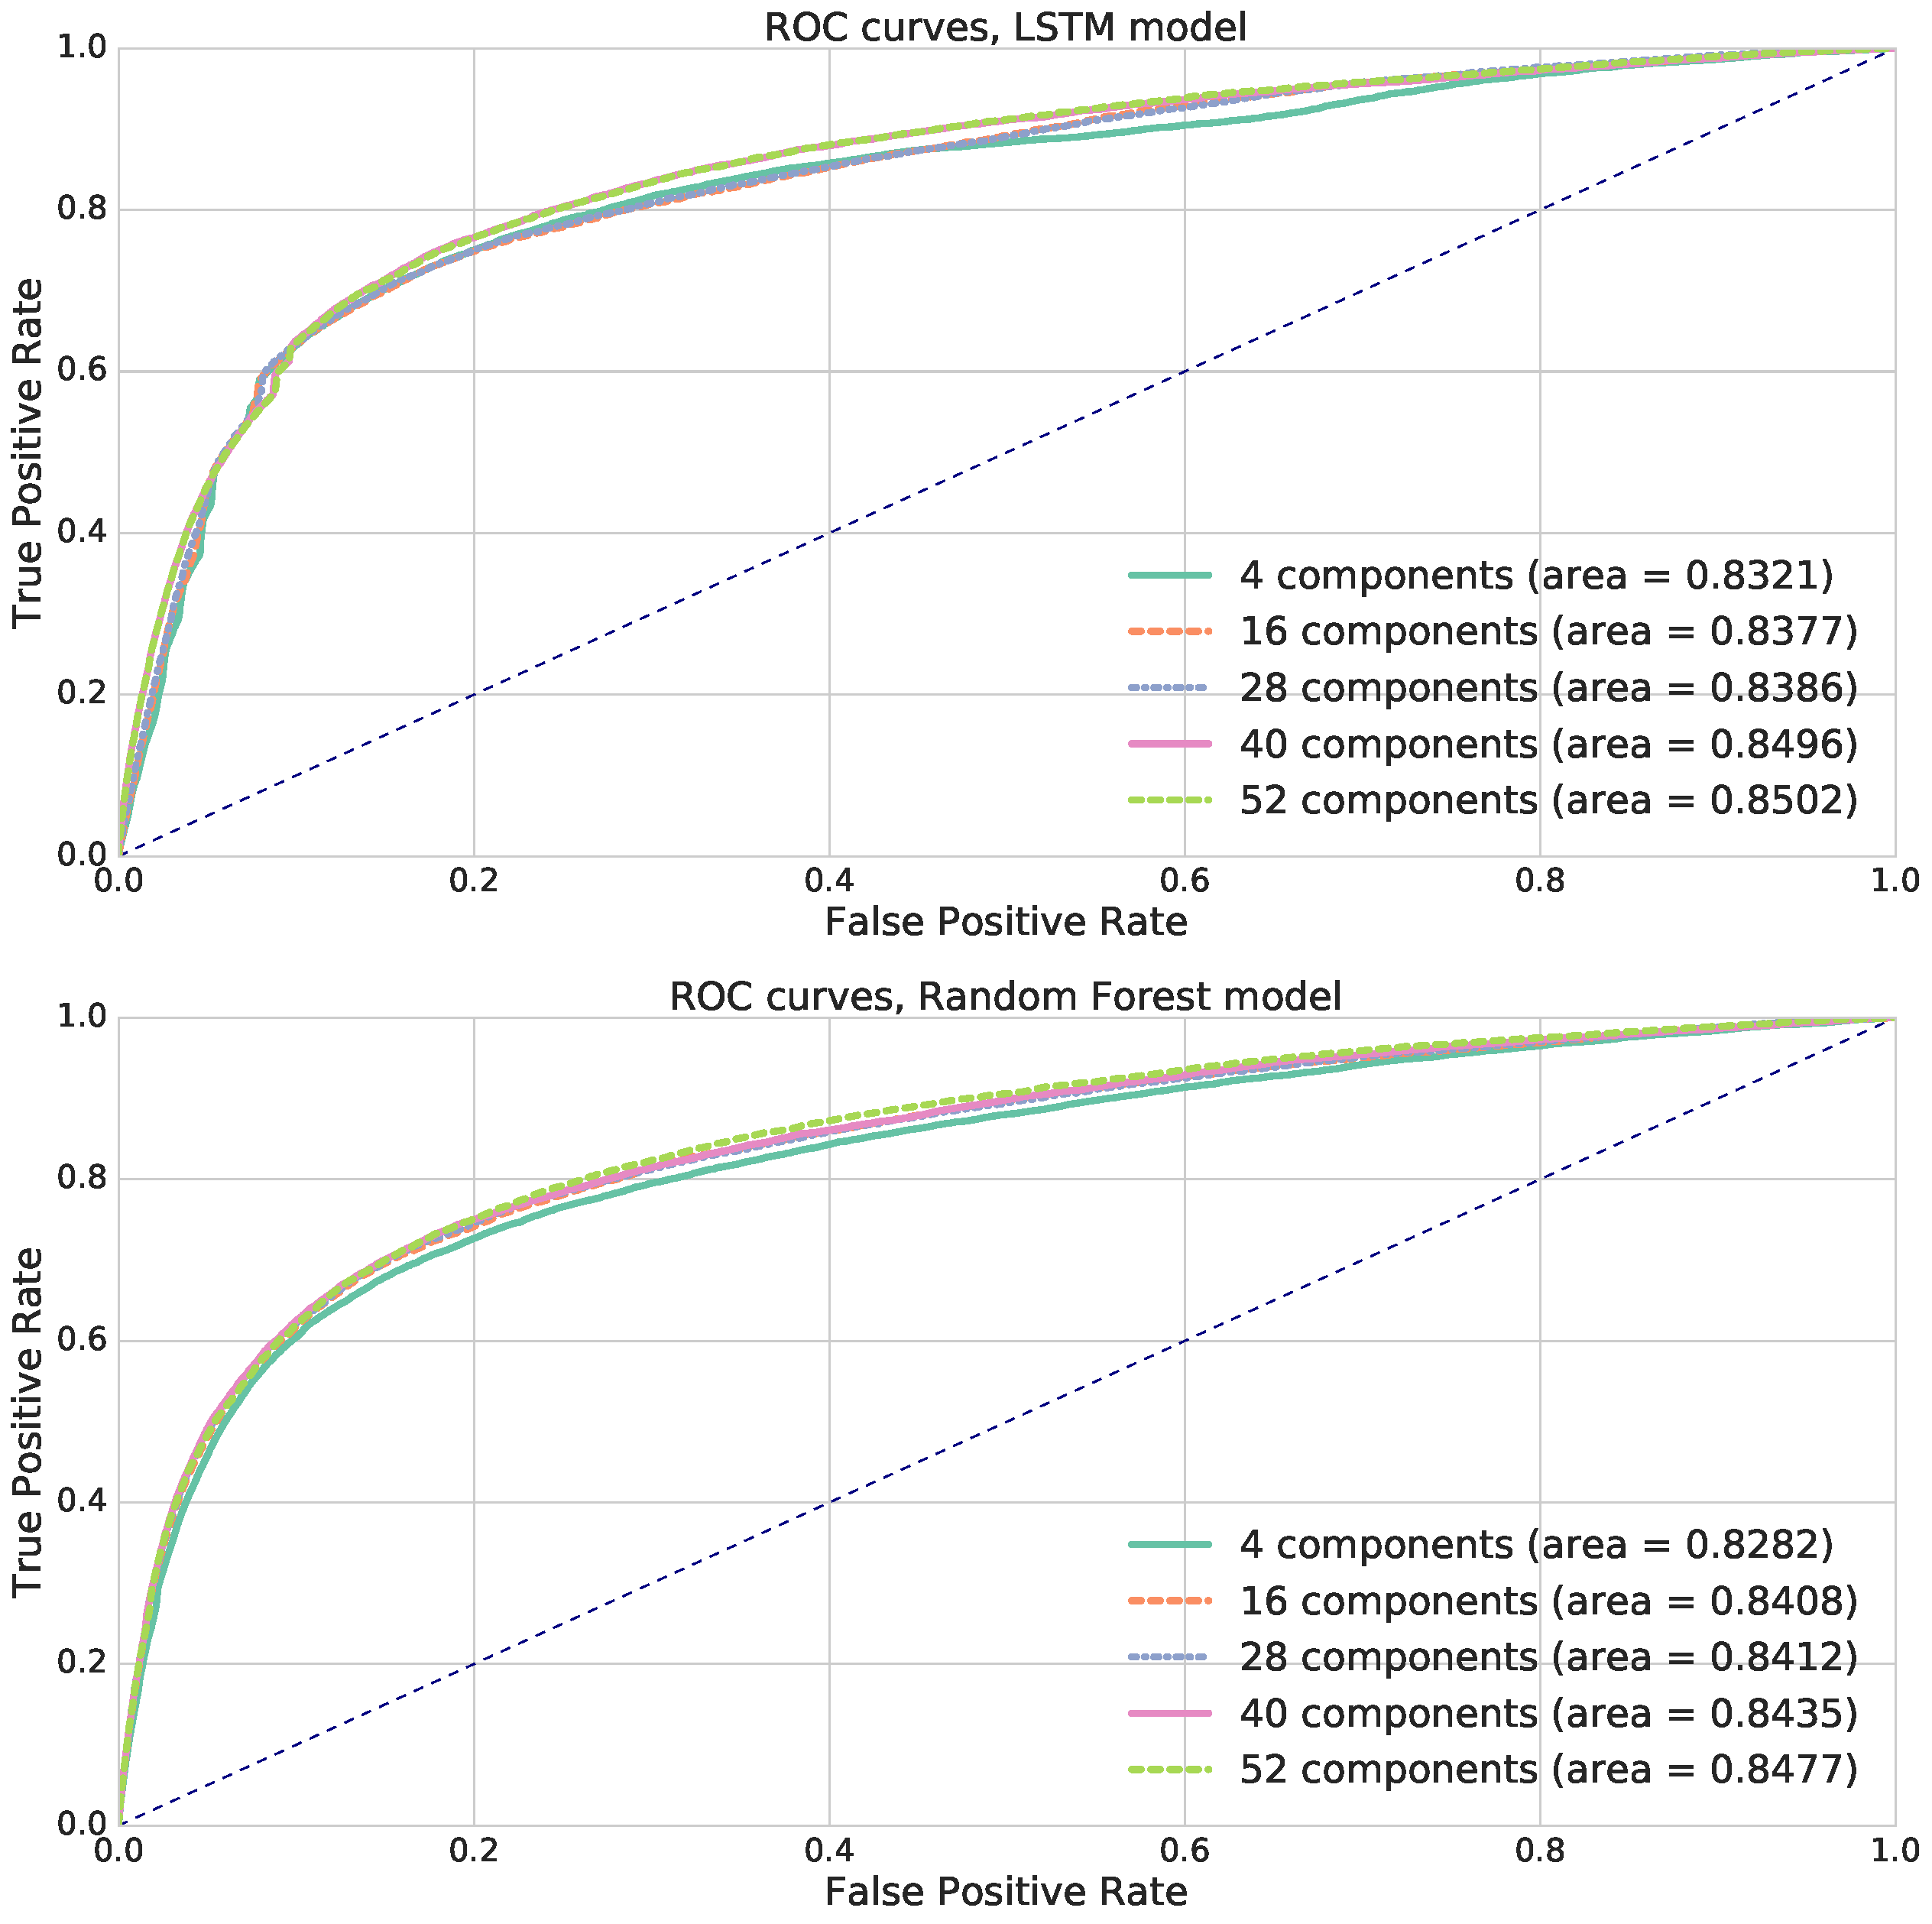
\includegraphics[width=1.0\textwidth,keepaspectratio]{figures/roc_dim_reduction.pdf}
    \caption{ROC curves for the dimensionality reduction experiment}
    \label{fig:roc_dim_reduction}
\end{figure}

% --------------------

\section{Metrics tables}


% --------------------

\begin{table}
\centering
\begin{tabular}{lllrrrr}
\toprule
     &   &          &  F1-Score &    PR AUC &  Precision &    Recall \\
Models & Days & Label &           &           &            &           \\
\midrule
\multirow{8}{*}{LSTM} & \multirow{2}{*}{7} & Retained &  0.864030 &  0.984615 &   0.979584 &  0.772862 \\
     &   & Churned &  \textbf{0.338950} &  \textit{0.333207} &   \textbf{0.215412} &  \textbf{0.794727} \\
\cline{2-7}
     & \multirow{2}{*}{14} & Retained &  0.903476 &  0.992219 &   0.988370 &  0.832012 \\
     &   & Churned &  0.256053 &  0.255312 &   0.154062 &  0.757580 \\
\cline{2-7}
     & \multirow{2}{*}{21} & Retained &  0.911840 &  0.994085 &   0.991263 &  0.844199 \\
     &   & Churned &  0.213510 &  0.213452 &   0.124511 &  0.748618 \\
\cline{2-7}
     & \multirow{2}{*}{28} & Retained &  \textbf{0.920708} &  \textit{0.994217} &   \textit{0.992211} &  \textbf{0.858818} \\
     &   & Churned &  0.195579 &  0.179993 &   0.112980 &  0.727317 \\
\cline{1-7}
\cline{2-7}
\multirow{8}{*}{Random Forest} & \multirow{2}{*}{7} & Retained &  0.859076 &  0.984100 &   0.979099 &  0.765265 \\
     &   & Churned &  \textit{0.331079} &  \textbf{0.333607} &   \textit{0.209295} &  \textit{0.791815} \\
\cline{2-7}
     & \multirow{2}{*}{14} & Retained &  0.889945 &  0.991412 &   0.988637 &  0.809169 \\
     &   & Churned &  0.237010 &  0.259038 &   0.140071 &  0.769709 \\
\cline{2-7}
     & \multirow{2}{*}{21} & Retained &  0.899322 &  0.993527 &   0.991293 &  0.822968 \\
     &   & Churned &  0.195370 &  0.227368 &   0.112185 &  0.755783 \\
\cline{2-7}
     & \multirow{2}{*}{28} & Retained &  \textit{0.907344} &  \textbf{0.994559} &   \textbf{0.992572} &  \textit{0.835596} \\
     &   & Churned &  0.177947 &  0.198052 &   0.101002 &  0.747073 \\
\cline{1-7}
\cline{2-7}
\multirow{8}{*}{Logistic Regression} & \multirow{2}{*}{7} & Retained &  0.819430 &  0.980246 &   0.973687 &  \textit{0.707365} \\
     &   & Churned &  \textit{0.275769} &  \textit{0.231384} &   \textit{0.168623} &  \textit{0.756390} \\
\cline{2-7}
     & \multirow{2}{*}{14} & Retained &  \textit{0.823319} &  0.988834 &   0.984885 &  0.707291 \\
     &   & Churned &  0.162862 &  0.140317 &   0.091636 &  0.731201 \\
\cline{2-7}
     & \multirow{2}{*}{21} & Retained &  0.821328 &  0.991033 &   0.987873 &  0.702837 \\
     &   & Churned &  0.120611 &  0.106732 &   0.065916 &  0.708495 \\
\cline{2-7}
     & \multirow{2}{*}{28} & Retained &  0.816645 &  \textit{0.992240} &  \textit{0.989444} &  0.695228 \\
     &   & Churned &  0.099809 &  0.084523 &   0.053735 &  0.700000 \\
\bottomrule
\end{tabular}
\caption{Metrics for the prediction window experiment}
\label{tab:pred_window}
\end{table}

% --------------------

\begin{table}
\centering
\begin{tabular}{lllrrrr}
\toprule
     &   &          &  F1-Score &    PR AUC &  Precision &    Recall \\
Models & Days & Label &           &           &            &           \\
\midrule
\multirow{16}{*}{LSTM} & \multirow{2}{*}{7} & Retained &  0.895413 &  0.992923 &   0.990665 &  0.816872 \\
     &   & Churned &  0.155974 &  0.126967 &   0.087826 &  0.696106 \\
\cline{2-7}
     & \multirow{2}{*}{14} & Retained &  0.886632 &  0.993870 &   \textbf{0.991997} &  0.801501 \\
     &   & Churned &  0.155449 &  0.155895 &   0.086782 &  \textbf{0.744706} \\
\cline{2-7}
     & \multirow{2}{*}{21} & Retained &  0.923889 &  0.993570 &   0.990672 &  0.865541 \\
     &   & Churned &  0.194156 &  0.138192 &   0.113294 &  0.678247 \\
\cline{2-7}
     & \multirow{2}{*}{28} & Retained &  0.907956 &  0.994128 &   0.991705 &  0.837250 \\
     &   & Churned &  0.177579 &  0.162224 &   0.101209 &  0.723529 \\
\cline{2-7}
     & \multirow{2}{*}{35} & Retained &  0.893332 &  0.993526 &   0.991655 &  0.812749 \\
     &   & Churned &  0.160036 &  0.169727 &   0.089869 &  0.729970 \\
\cline{2-7}
     & \multirow{2}{*}{42} & Retained &  0.899900 &  0.993773 &  0.991808 &  0.823580 \\
     &   & Churned &  0.168215 &  \textit{0.175214} &   0.095036 &  0.731434 \\
\cline{2-7}
     & \multirow{2}{*}{49} & Retained &  \textbf{0.934375} &  \textit{0.994084} &   0.990261 &  \textbf{0.884461} \\
     &   & Churned &  \textbf{0.211187} &  0.153296 &   \textbf{0.125830} &  0.656582 \\
\cline{2-7}
     & \multirow{2}{*}{56} & Retained &  0.911085 &  0.994052 &   0.991691 &  0.842597 \\
     &   & Churned &  0.181787 &  0.174330 &   0.103999 &  0.721284 \\
\cline{1-7}
\cline{2-7}
\multirow{16}{*}{Random Forest} & \multirow{2}{*}{7} & Retained &  0.876067 &  0.993260 &   0.991120 &  0.784947 \\
     &   & Churned &  0.141465 &  0.140472 &   0.078410 &  0.722358 \\
\cline{2-7}
     & \multirow{2}{*}{14} & Retained &  0.890595 &  0.993833 &   0.991612 &  0.808257 \\
     &   & Churned &  0.157004 &  0.171877 &   0.087960 &  0.730067 \\
\cline{2-7}
     & \multirow{2}{*}{21} & Retained &  0.893176 &  0.993899 &   0.991700 &  0.812459 \\
     &   & Churned &  0.160150 &  0.188480 &   0.089918 &  0.731531 \\
\cline{2-7}
     & \multirow{2}{*}{28} & Retained &  0.893712 &  0.994151 &   \textit{0.991931} &  0.813191 \\
     &   & Churned &  0.162136 &  0.196100 &   0.091059 &  \textit{0.738850} \\
\cline{2-7}
     & \multirow{2}{*}{35} & Retained &  0.898663 &  0.994214 &   0.991843 &  0.821487 \\
     &   & Churned &  0.167019 &  0.201898 &   0.094242 &  0.733288 \\
\cline{2-7}
     & \multirow{2}{*}{42} & Retained &  0.898192 &  0.994117 &   0.991803 &  0.820728 \\
     &   & Churned &  0.166227 &  \textbf{0.202974} &   0.093756 &  0.732214 \\
\cline{2-7}
     & \multirow{2}{*}{49} & Retained &  \textit{0.900939} &  0.993919 &   0.991547 &  \textit{0.825504} \\
     &   & Churned &  \textit{0.167726} &  0.201751 &   \textit{0.094882} &  0.722163 \\
\cline{2-7}
     & \multirow{2}{*}{56} & Retained &  0.896787 &  \textbf{0.994241} &   0.991866 &  0.818342 \\
     &   & Churned &  0.165052 &  0.200151 &   0.092964 &  0.735044 \\
\cline{1-7}
\cline{2-7}
\multirow{16}{*}{Logistic Regression} & \multirow{2}{*}{7} & Retained &  0.813596 &  0.991253 &   0.988041 &  0.691507 \\
     &   & Churned &  0.096696 &  0.076120 &   0.052111 &  0.669562 \\
\cline{2-7}
     & \multirow{2}{*}{14} & Retained &  0.825077 &  0.991869 &   0.989111 &  0.707710 \\
     &   & Churned &  0.104656 &  0.088905 &   0.056606 &  0.692398 \\
\cline{2-7}
     & \multirow{2}{*}{21} & Retained &  0.826441 &  0.992184 &   0.989862 &  0.709334 \\
     &   & Churned &  0.108152 &  0.096097 &   0.058513 &  0.713184 \\
\cline{2-7}
     & \multirow{2}{*}{28} & Retained &  0.829275 &  0.992497 &   0.990268 &  0.713309 \\
     &   & Churned &  0.110912 &  0.100216 &   0.060061 &  0.723236 \\
\cline{2-7}
     & \multirow{2}{*}{35} & Retained &  0.830033 &  0.992643 &   0.990586 &  0.714266 \\
     &   & Churned &  0.112509 &  0.103061 &   0.060937 &  0.732019 \\
\cline{2-7}
     & \multirow{2}{*}{42} & Retained &  0.829788 &  0.992641 &   0.990720 &  0.713833 \\
     &   & Churned &  0.112941 &  0.101419 &   0.061163 &  0.736020 \\
\cline{2-7}
     & \multirow{2}{*}{49} & Retained &  \textit{0.834670} &  0.992744 &   0.990785 &  \textit{0.721056} \\
     &   & Churned &  \textit{0.115351} &  \textit{0.104809} &   \textit{0.062585} &  0.735240 \\
\cline{2-7}
     & \multirow{2}{*}{56} & Retained &  0.830928 &  \textit{0.992801} &   \textit{0.991129} &  0.715309 \\
     &   & Churned &  0.115078 &  0.103800 &   0.062339 &  \textit{0.747243} \\
\bottomrule
\end{tabular}
\caption{Metrics for the observation window experiment}
\label{tab:obs_window}
\end{table}

%---------------------

\begin{table}
\centering
\begin{tabular}{lllrrrr}
\toprule
     &     &          &  F1-Score &    PR AUC &  Precision &    Recall \\
Models & Share & Label &           &           &            &           \\
\midrule
\multirow{18}{*}{LSTM} & \multirow{2}{*}{10\%} & Retained &  \textbf{0.982307} &  0.994025 &   0.983159 &  \textbf{0.981457} \\
     &     & Churned &  \textbf{0.307656} &  0.217342 &   \textbf{0.297570} &  0.318449 \\
\cline{2-7}
     & \multirow{2}{*}{15\%} & Retained &  0.975857 &  0.994287 &   0.985437 &  0.966461 \\
     &     & Churned &  0.302806 &  0.222597 &   0.236429 &  0.421001 \\
\cline{2-7}
     & \multirow{2}{*}{20\%} & Retained &  0.962595 &  0.994362 &   0.988227 &  0.938260 \\
     &     & Churned &  0.270067 &  0.224562 &   0.179310 &  0.546860 \\
\cline{2-7}
     & \multirow{2}{*}{25\%} & Retained &  0.966747 &  0.993023 &   0.987343 &  0.946993 \\
     &     & Churned &  0.277759 &  0.201470 &   0.191153 &  0.507851 \\
\cline{2-7}
     & \multirow{2}{*}{30\%} & Retained &  0.943058 &  0.994174 &   0.990025 &  0.900346 \\
     &     & Churned &  0.222924 &  0.194165 &   0.135318 &  0.632237 \\
\cline{2-7}
     & \multirow{2}{*}{35\%} & Retained &  0.941206 &  0.994706 &   0.990460 &  0.896618 \\
     &     & Churned &  0.222530 &  \textbf{0.223431} &   0.134249 &  0.649902 \\
\cline{2-7}
     & \multirow{2}{*}{40\%} & Retained &  0.930454 &  \textbf{0.994734} &   0.991322 &  0.876629 \\
     &     & Churned &  0.205941 &  0.220575 &   0.121066 &  0.688911 \\
\cline{2-7}
     & \multirow{2}{*}{45\%} & Retained &  0.923512 &  0.994291 &   0.991447 &  0.864289 \\
     &     & Churned &  0.193832 &  0.175024 &   0.112549 &  0.697743 \\
\cline{2-7}
     & \multirow{2}{*}{50\%} & Retained &  0.914968 &  0.994161 &   \textit{0.991891} &  0.849117 \\
     &     & Churned &  0.183424 &  0.184284 &   0.105129 &  \textit{0.718597} \\
\cline{1-7}
\cline{2-7}
\multirow{18}{*}{Random Forest} & \multirow{2}{*}{10\%} & Retained &  \textit{0.981921} &  0.993655 &   0.983035 &  \textit{0.980810} \\
     &     & Churned &  \textit{0.300023} &  0.203894 &   \textit{0.287416} &  0.313788 \\
\cline{2-7}
     & \multirow{2}{*}{15\%} & Retained &  0.974738 &  0.993544 &   0.985423 &  0.964282 \\
     &     & Churned &  0.293922 &  0.204665 &   0.225561 &  0.421737 \\
\cline{2-7}
     & \multirow{2}{*}{20\%} & Retained &  0.961760 &  \textit{0.993784} &   0.987977 &  0.936898 \\
     &     & Churned &  0.262594 &  0.209803 &   0.173706 &  0.537782 \\
\cline{2-7}
     & \multirow{2}{*}{25\%} & Retained &  0.961340 &  0.993670 &   0.988060 &  0.936027 \\
     &     & Churned &  0.261896 &  \textit{0.212639} &   0.172719 &  0.541462 \\
\cline{2-7}
     & \multirow{2}{*}{30\%} & Retained &  0.951873 &  0.993767 &   0.989192 &  0.917266 \\
     &     & Churned &  0.239996 &  0.209713 &   0.150395 &  0.593719 \\
\cline{2-7}
     & \multirow{2}{*}{35\%} & Retained &  0.943922 &  0.993684 &   0.989599 &  0.902276 \\
     &     & Churned &  0.220736 &  0.207393 &   0.134480 &  0.615554 \\
\cline{2-7}
     & \multirow{2}{*}{40\%} & Retained &  0.933831 &  0.993775 &   0.990513 &  0.883286 \\
     &     & Churned &  0.205684 &  0.210247 &   0.121927 &  0.657017 \\
\cline{2-7}
     & \multirow{2}{*}{45\%} & Retained &  0.916083 &  0.993626 &   0.991306 &  0.851471 \\
     &     & Churned &  0.180668 &  0.208895 &   0.103779 &  0.697252 \\
\cline{2-7}
     & \multirow{2}{*}{50\%} & Retained &  0.896975 &  0.993761 &   \textbf{0.992056} &  0.818526 \\
     &     & Churned &  0.161539 &  0.208957 &   0.090752 &  \textbf{0.734298} \\
\bottomrule
\end{tabular}
\caption{Metrics for the class balance experiment}
\label{tab:class_balance}
\end{table}

%---------------------

\begin{table}
\centering
\begin{tabular}{lllrrrr}
\toprule
     &   &          &  F1-Score &    PR AUC &  Precision &    Recall \\
Models & \# Components & Label &           &           &            &           \\
\midrule
\multirow{10}{*}{LSTM} & \multirow{2}{*}{4} & Retained &  0.922415 &  0.993324 &   0.990890 &  0.862792 \\
     &   & Churned &  0.193373 &  0.140500 &   0.112527 &  0.686835 \\
\cline{2-7}
     & \multirow{2}{*}{16} & Retained &  \textbf{0.927496} &  0.993826 &   0.990609 &  \textbf{0.871943} \\
     &   & Churned &  \textbf{0.200218} &  0.146970 &   \textbf{0.117582} &  0.673661 \\
\cline{2-7}
     & \multirow{2}{*}{28} & Retained &  0.924869 &  0.993922 &   0.990807 &  0.867160 \\
     &   & Churned &  0.197016 &  0.152360 &   0.115129 &  0.682346 \\
\cline{2-7}
     & \multirow{2}{*}{40} & Retained &  0.902679 &  0.994233 &   0.992157 &  0.828005 \\
     &   & Churned &  0.173838 &  \textit{0.185674} &   0.098459 &  0.741583 \\
\cline{2-7}
     & \multirow{2}{*}{52} & Retained &  0.898539 &  \textbf{0.994353} &   \textbf{0.992256} &  0.820997 \\
     &   & Churned &  0.169514 &  0.184844 &   0.095604 &  \textbf{0.747048} \\
\cline{1-7}
\cline{2-7}
\multirow{10}{*}{Random Forest} & \multirow{2}{*}{4} & Retained &  0.886591 &  0.993103 &   0.991396 &  0.801825 \\
     &   & Churned &  0.151906 &  0.175956 &   0.084837 &  0.725285 \\
\cline{2-7}
     & \multirow{2}{*}{16} & Retained &  0.903003 &  0.993781 &   0.991422 &  0.829063 \\
     &   & Churned &  0.169349 &  0.192872 &   0.096017 &  0.716795 \\
\cline{2-7}
     & \multirow{2}{*}{28} & Retained &  \textit{0.906450} &  0.993801 &   0.991455 &  \textit{0.834870} \\
     &   & Churned &  0.173868 &  0.193854 &   0.098949 &  0.715917 \\
\cline{2-7}
     & \multirow{2}{*}{40} & Retained &  0.906357 &  0.993904 &   0.991499 &  0.834682 \\
     &   & Churned &  \textit{0.174057} &  0.196415 &   \textit{0.099042} &  0.717478 \\
\cline{2-7}
     & \multirow{2}{*}{52} & Retained &  0.895238 &  \textit{0.994219} &   \textit{0.991906} &  0.815740 \\
     &   & Churned &  0.163607 &  \textbf{0.196442} &   0.092014 &  \textit{0.737191} \\
\bottomrule
\end{tabular}
\caption{Metrics for the dimensionality reduction experiment}
\label{tab:dim_reduction}
\end{table}

\todos

\end{document}
